% ===================================================================
%  DATATHON 2026 — THE GRIDBREAKERS
%  NeurIPS 2025 Template — Main Body ≤ 4 pages, Appendix unlimited
% ===================================================================
\documentclass{article}
\def\@trackname{}
\usepackage[final,main]{neurips_2025}

\usepackage[utf8]{inputenc}
\usepackage[T1]{fontenc}
\usepackage[vietnamese]{babel}
\usepackage{hyperref}
\usepackage{url}
\usepackage{booktabs}
\usepackage{amsfonts}
\usepackage{nicefrac}
\usepackage{microtype}
\usepackage{xcolor}
\usepackage{graphicx}
\usepackage{amsmath}
\usepackage{subcaption}
\usepackage{multirow}
\usepackage{array}
\usepackage{enumitem}
\usepackage{float}
\setlist[itemize]{noitemsep, topsep=1pt, leftmargin=*}
\setlist[enumerate]{noitemsep, topsep=1pt, leftmargin=*}

\definecolor{vinblue}{RGB}{41,98,255}
\definecolor{vingray}{RGB}{100,100,100}
\hypersetup{colorlinks=true,linkcolor=vinblue,urlcolor=vinblue,citecolor=vingray}

% ── Tighten spacing throughout ───────────────────────────────────────
\setlength{\floatsep}{3pt plus 1pt minus 1pt}
\setlength{\textfloatsep}{4pt plus 1pt minus 1pt}
\setlength{\intextsep}{3pt plus 1pt minus 1pt}
\setlength{\abovecaptionskip}{2pt}
\setlength{\belowcaptionskip}{0pt}
\setlength{\abovedisplayskip}{4pt}
\setlength{\belowdisplayskip}{4pt}

% ===================================================================
\title{Dự Báo Doanh Thu Thương Mại Điện Tử Thời Trang:\\
       Pipeline Lịch Thuần Tuý Kết Hợp Hiệu Chỉnh Tăng Trưởng YoY}

\author{%
  Trương Nguyên Đại Thắng\thanks{Nhóm trưởng. GitHub: \url{https://github.com/inwinnieworld/DatathonTop}} \And
  Lê Thị Hồng Đang \And
  Lương Thị Hồng Nhung \And
  Trần Võ Minh Hùng \\[2pt]
  \texttt{Datathon 2026 — The Gridbreakers | VinTelligence × VinUniversity DS\&AI Club}
}

\begin{document}
\maketitle

% ===================================================================
\begin{abstract}
Chúng tôi trình bày hệ thống dự báo doanh thu và COGS hàng ngày cho doanh nghiệp thời trang TMĐT Việt Nam, giai đoạn 01/01/2023–01/07/2024, huấn luyện trên lịch sử 2012–2022 (3.833 ngày, 14 bảng dữ liệu). Pipeline gồm ba lớp: (1)~94 đặc trưng lịch thuần tuý tính trước hoàn toàn; (2)~ensemble LightGBM Q-Specialist đa seed kết hợp Ridge và Prophet; (3)~hệ số hiệu chỉnh CR suy diễn từ tăng trưởng YoY ngành TMĐT theo báo cáo MoIT 2022. Mô hình tốt nhất (v47, 10 seeds) đạt \textbf{MAE = 669.087} trên leaderboard. Phân tích SHAP xác nhận Fourier năm (31,5\%) và xu hướng thời gian (21,9\%) là hai driver chính, với Urban Blowout được nhận diện đúng là sự kiện margin âm.
\end{abstract}

% ===================================================================
\section{Bối Cảnh Kinh Doanh \& Mô Tả Dữ Liệu}
% ===================================================================

\textbf{Mô hình kinh doanh.} Doanh nghiệp vận hành theo mô hình \textit{pure-play e-commerce} thời trang tại Việt Nam: 4 danh mục sản phẩm (Streetwear 54,7\%, Outdoor 30,8\%, Casual 8,3\%, GenZ 6,1\%), 3 vùng địa lý, 5 phương thức thanh toán và trả góp 12 kỳ. Revenue từ bán lẻ, phí ship và CLV; chi phí chính gồm COGS, logistics và chiết khấu khuyến mãi (Hình~\ref{fig:bmc}, Phụ lục~A).

\textbf{Bộ dữ liệu.} 15 file CSV: 4 bảng master, 6 bảng transaction, sales.csv (train: 04/07/2012–31/12/2022), web\_traffic.csv và inventory.csv. Kiểm tra toàn vẹn: không có ngày thiếu, COGS < price với mọi dòng, promo\_id null = 61,3\% (phần lớn đơn không áp khuyến mãi — hợp lệ).

% ===================================================================
\section{Phân Tích Dữ Liệu Khám Phá (EDA)}
% ===================================================================

\vspace{-2pt}
\subsection{Mô Tả — \textit{Điều gì đã xảy ra?}}
\vspace{-2pt}

Bảng~\ref{tab:desc} tổng hợp các chỉ số tài chính. CV của Revenue = 61,2\% phản ánh biến động mạnh theo mùa vụ. Gross Margin có skewness âm sâu ($-2,532$), min $= -57,46\%$, báo hiệu tồn tại giao dịch lỗ gộp cần điều tra.

\begin{table}[h!]
\centering
\caption{Thống kê mô tả chỉ số tài chính cốt lõi (3.833 ngày, 2012–2022)}
\label{tab:desc}
\footnotesize
\setlength{\tabcolsep}{4pt}
\begin{tabular}{lrrrrrr}
\toprule
\textbf{Chỉ số} & \textbf{Mean} & \textbf{Std} & \textbf{Min} & \textbf{Median} & \textbf{Skew} & \textbf{CV(\%)} \\
\midrule
Revenue (VNĐ)      & 4.286.584 & 2.624.840 & 279.814  & 3.647.304 & 1,67  & 61,2 \\
COGS (VNĐ)         & 3.695.134 & 2.219.789 & 236.576  & 3.161.113 & 1,63  & 60,1 \\
Gross Profit (VNĐ) & 591.450   & 666.196   & $-$2.567.312 & 544.554 & 8,24 & 112,6 \\
Gross Margin (\%)  & 12,54     & 12,74     & $-$57,46 & 17,83     & $-$2,53 & 101,6 \\
\bottomrule
\end{tabular}
\end{table}

\textbf{Mùa vụ \& Xu hướng.} Seasonality index dao động 0,58 (T12) đến 1,52 (T5) — tháng đỉnh cao hơn đáy 2,6×. Xu hướng theo hình chữ U ngược: đỉnh 2016 (5,75M/ngày) → đáy 2021 (2,86M) → phục hồi 2022 (+12,1\%). Chi tiết tại Hình~\ref{fig:ts_main}–\ref{fig:decompose} (Phụ lục~A).

\vspace{-2pt}
\subsection{Chẩn Đoán — \textit{Tại sao xảy ra?}}
\vspace{-2pt}

\textbf{Dịch chuyển cấu trúc 2019.} Doanh thu sụt $-38,6\%$ trong một năm. Decomposition (Hình~\ref{fig:decompose}) xác nhận: trend giảm đột ngột, seasonal component ổn định — \textit{level} thay đổi, \textit{shape} không đổi. Đây là cơ sở thiết kế CR calibration tách riêng khỏi shape model.

\textbf{Nghịch lý Urban Blowout.} Hình~\ref{fig:cogs_margin} cho thấy Q3 năm lẻ có COGS/Rev = 1,057 — chiến dịch Urban Blowout giảm giá sâu làm COGS vượt Revenue. Phân tích discount (Hình~\ref{fig:discount}, Phụ lục~A): percentage-type discount chiếm 14,7\% net revenue, cao hơn fixed-type (1,3\%). Nghịch lý này trực tiếp dẫn đến công thức CC per-segment theo quý × năm lẻ/chẵn (Bảng~\ref{tab:margin_qparity}, Phụ lục~B).

\textbf{Khủng hoảng giữ chân khách hàng \& Tồn kho.} Cohort retention $\approx 0\%$ sau M+1 (Hình~\ref{fig:cohort}, Phụ lục~A); inter-order gap trung vị = 146 ngày, mean = 288 ngày. CLV đồng đều qua kênh acquisition (170K–175K) — vấn đề nằm ở trải nghiệm sau mua, không phải kênh. Sell-through rate 20\% với fill rate 95\% — 75\% tồn kho không tiêu thụ, trong khi SKU rating cao lại hay stockout nhất (Hình~\ref{fig:inventory}, Phụ lục~A).

\begin{figure}[t]
\centering
\begin{subfigure}[b]{0.52\linewidth}
  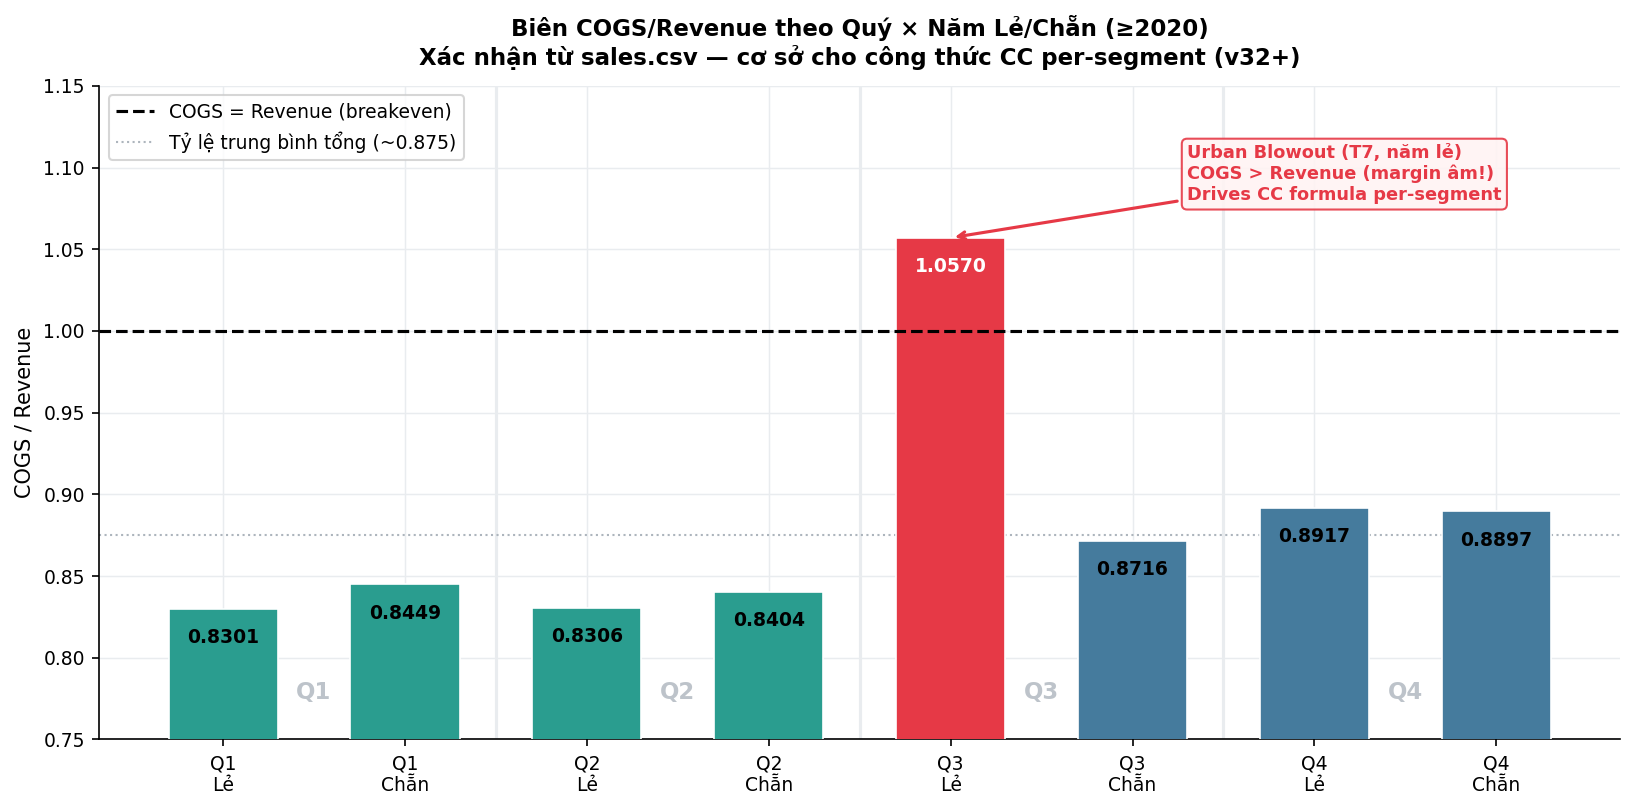
\includegraphics[width=\linewidth]{figures/modelling/fig3_cogs_margin_by_quarter_parity.png}
  \caption{COGS/Revenue theo Quý × Năm Lẻ/Chẵn}
  \label{fig:cogs_margin}
\end{subfigure}%
\hfill%
\begin{subfigure}[b]{0.46\linewidth}
  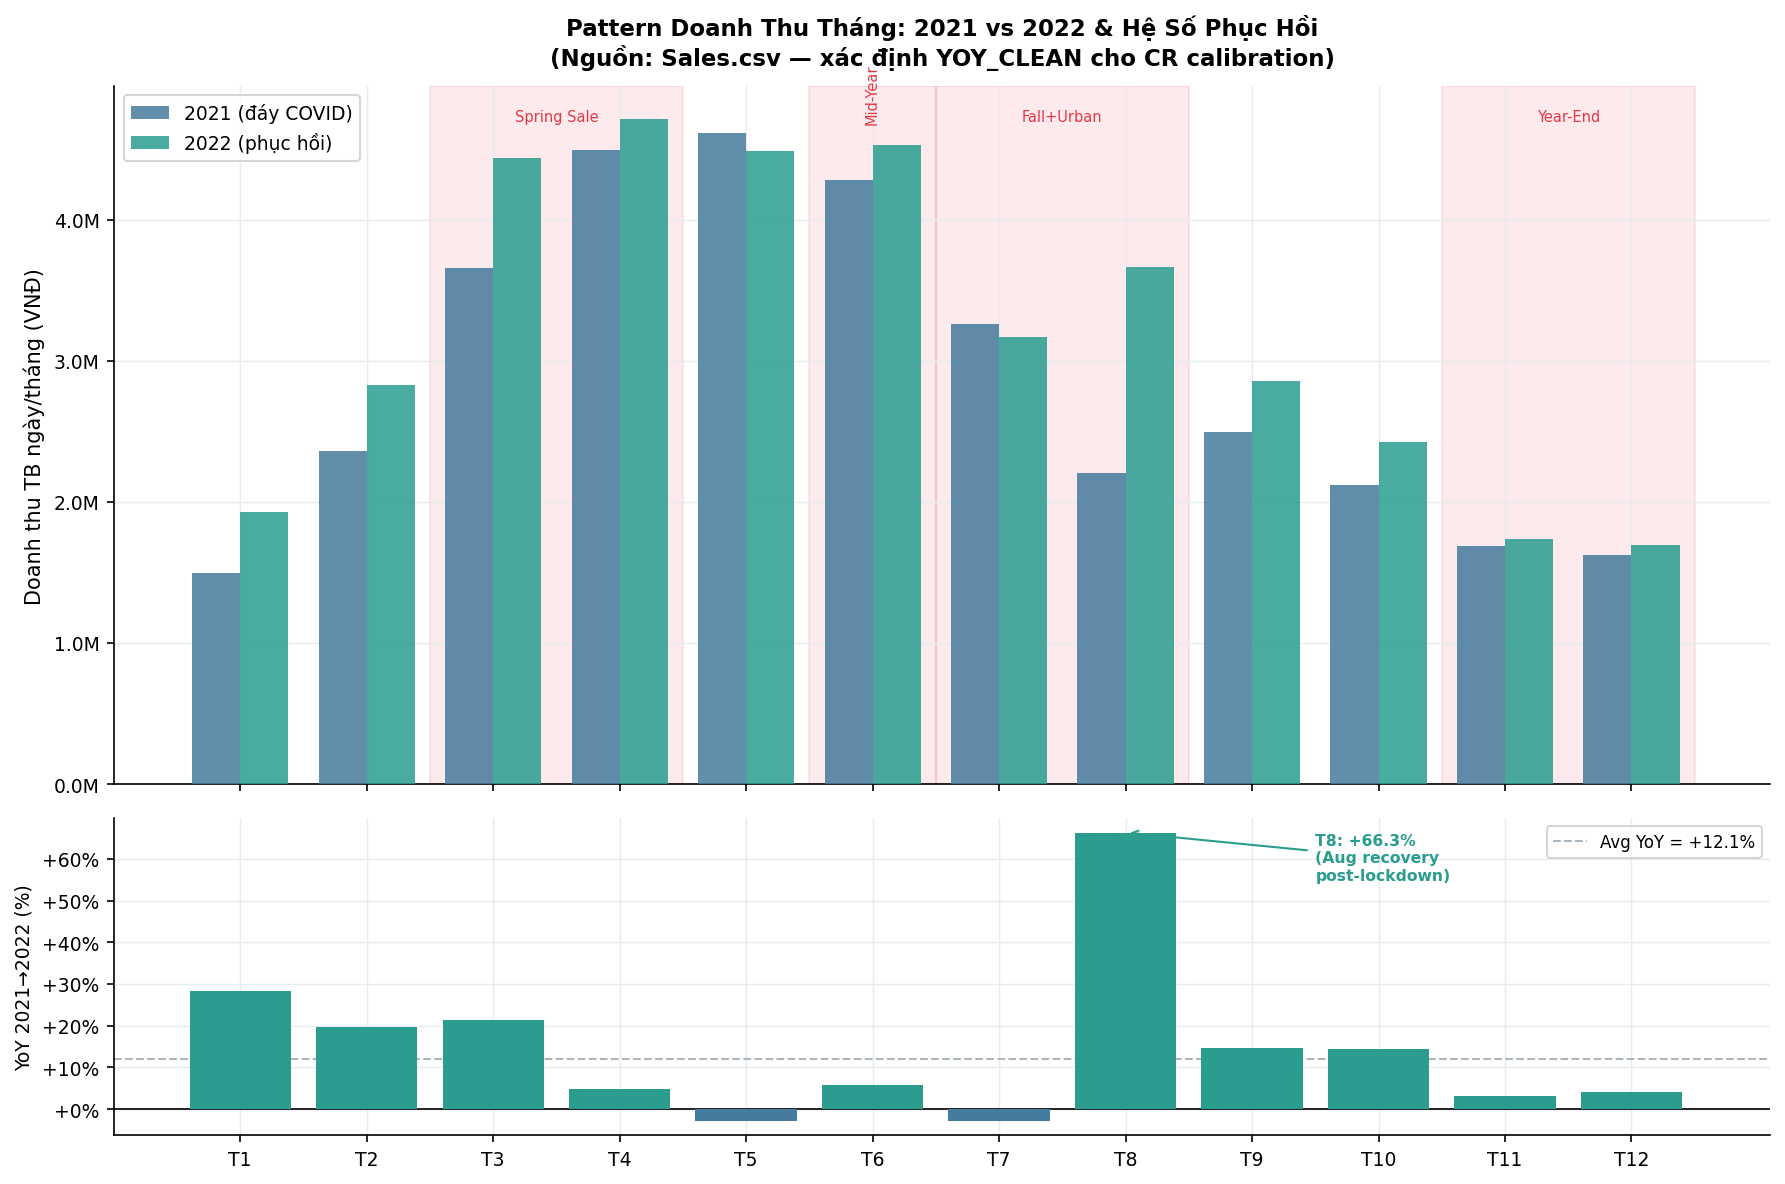
\includegraphics[width=\linewidth]{figures/modelling/fig2_monthly_recovery_pattern.png}
  \caption{Hệ số phục hồi tháng 2021$\to$2022}
  \label{fig:monthly_recovery}
\end{subfigure}
\caption{\textbf{Chẩn đoán margin và phục hồi.} (a)~Q3 năm lẻ = 1,057 (lỗ gộp) — cơ sở CC per-segment. (b)~Phục hồi 2022 không đều: T8 đột biến +66,3\% (post-lockdown); T5, T7 vẫn âm.}
\label{fig:diagnostic}
\vspace{-4pt}
\end{figure}

\vspace{-2pt}
\subsection{Dự Báo — \textit{Điều gì có thể xảy ra?}}
\vspace{-2pt}

Pattern mùa vụ bền vững qua mọi era (kể cả COVID): đỉnh T4–T6, đáy T11–T1 — có thể mô hình hoá bằng Fourier mà không cần lag. Sessions–Revenue $r=0,32$, bounce rate $r=-0,02$ (Hình~\ref{fig:corr}, Phụ lục~A) — conversion funnel quan trọng hơn traffic volume. Streetwear tăng từ 75\% (2012) lên 84\% (2022), Outdoor giảm từ 22\% xuống 9\% — nguy cơ tiếp tục suy giảm nếu không tái định vị (Hình~\ref{fig:stacked}, Phụ lục~A).

\vspace{-6pt} % Ép khoảng cách để chống ugly blanks
\subsection{Đề Xuất Hành Động — \textit{Doanh nghiệp cần làm gì? (Prescriptive)}}
\vspace{-2pt}

Tổng hợp từ các đứt gãy trong phễu chuyển đổi (Traffic) và chuỗi cung ứng (Supply Chain), Bảng \ref{tab:prescriptive} lượng hóa các rủi ro và đề xuất các hành động chiến lược (Actionable Insights) nhằm xoay trục biên lợi nhuận.

\begin{table}[H] % Dùng [htbp] thay vì [H] để LaTeX tự trôi bảng cho khít trang
\centering
\caption{Đề xuất hành động chiến lược dựa trên bằng chứng dữ liệu phân tích}
\label{tab:prescriptive}
\scriptsize
\setlength{\tabcolsep}{3pt}
\renewcommand{\arraystretch}{1.1}
\begin{tabular}{p{2.5cm} p{4.6cm} p{5.8cm}}
\toprule
\textbf{Nút thắt cốt lõi} & \textbf{Bằng chứng Dữ liệu (Data Evidence)} & \textbf{Hành động Đề xuất (Prescriptive Action)} \\
\midrule

\textbf{1. Lãng phí Traffic \& \newline Rớt khách hàng} & 
- Conversion Rate (CR) cực thấp: \textbf{1,1\%} \newline
- \textbf{90M} sessions bị lãng phí \newline
- Retention M+1 $< 4\%$ \newline
- 26\% khách bỏ cuộc ở đơn đầu tiên & 
\vspace{-8pt}\begin{itemize}
    \item \textbf{Tối ưu CRO:} Đơn giản hóa quy trình checkout, tăng tốc độ tải trang mobile.
    \item \textbf{Remarketing:} Đeo bám giỏ hàng (Browse Abandonment) cho 90M sessions.
    \item \textbf{Loyalty:} Xây dựng luồng tri ân riêng cho nhóm \textbf{55+} (nhóm có LTV cao nhất: 7,42 đơn/khách).
\end{itemize}\vspace{-8pt} \\

\midrule

\textbf{2. Biên lợi nhuận mỏng \newline \& Lỗ vận hành Q4} & 
- Discount ăn mòn \textbf{14,7\%} Net Revenue \newline
- Q4 là đáy mùa vụ (Lợi nhuận T12 chỉ 3 tỷ) \newline
- Tương quan COGS/Rev rất cao ($r=0,976$) & 
\vspace{-8pt}\begin{itemize}
    \item \textbf{Cắt giảm ngân sách:} Giảm chi phí Marketing \& nhân sự thời vụ trong Q4 để bảo vệ margin.
    \item \textbf{Cải cách Discount:} Ngừng chiến lược đổi volume lấy margin; giới hạn % discount cho các danh mục không sinh lời.
\end{itemize}\vspace{-8pt} \\

\midrule

\textbf{3. Đứt gãy Chuỗi cung ứng \newline \& Trả hàng} & 
- Stockout rate lên tới \textbf{67,34\%} \newline
- Sell-through chỉ \textbf{20\%} dù Fill rate 95\% \newline
- Sai kích cỡ chiếm \textbf{35\%} lý do trả hàng (đặc biệt size XL chiếm 3,7K case) & 
\vspace{-8pt}\begin{itemize}
    \item \textbf{AI Sizing:} Đầu tư công cụ gợi ý kích cỡ trực quan (ROI sẽ cao hơn việc tối ưu tốc độ giao hàng).
    \item \textbf{Audit kho bãi:} Rà soát hiện tượng tồn kho ảo (đặc biệt dòng BambooCraft). Ưu tiên nhập gấp các SKUs có Stockout Cost cao (HanoiStreet, DragonWear).
\end{itemize}\vspace{-8pt} \\

\midrule

\textbf{4. Mất cân bằng \newline Danh mục \& Phân khúc} & 
- \textbf{Standard:} Margin cao nhất (31,3\%) nhưng volume thấp \newline
- \textbf{Trendy:} Trả hàng cao nhất (3,52\%) \newline
- Quá phụ thuộc vào Streetwear (84\% Rev) & 
\vspace{-8pt}\begin{itemize}
    \item \textbf{Scale-up:} Dồn ngân sách Ads cho phân khúc Standard.
    \item \textbf{Kiểm định chất lượng:} Chuẩn hóa lại hình ảnh/mô tả thực tế cho nhóm Trendy để khớp kỳ vọng khách hàng.
\end{itemize}\vspace{-8pt} \\

\bottomrule
\end{tabular}
\end{table}

\vspace{-4pt} % Ép khoảng cách trước khi sang Phần 3

% ===================================================================
\section{Pipeline Mô Hình Dự Báo}
% ===================================================================

\vspace{-2pt}
\subsection{Feature Engineering — 94 Đặc Trưng Lịch Thuần Tuý}
\vspace{-2pt}

Toàn bộ 94 đặc trưng là \textit{calendar-only} — tính trước hoàn toàn, không cần lag, triệt tiêu data leakage. Sáu nhóm: Fourier mùa vụ (18: sin/cos năm k=1..5, tuần k=1..2, tháng k=1..2), Khuyến mãi (24: flag + \texttt{since}/\texttt{until}/\texttt{disc} cho 6 campaigns — \texttt{since}/\texttt{until} encode ramp-up và FOMO), Tết Nguyên Đán (9: \texttt{tet\_days\_diff}, \texttt{tet\_intensity} phi tuyến, in-7/14/30), EOM/Ngày lương (12: \texttt{days\_to\_eom}, \texttt{payday\_intensity} 5 mức), Xu hướng \& Chế độ (5: \texttt{t\_days/t\_years}, 3 regime flags), Lịch cơ bản \& Lễ (26). Danh sách đầy đủ tại Phụ lục~C. Lịch 6 chiến dịch khuyến mãi tái tạo hoàn toàn từ \texttt{promotions.csv} (Hình~\ref{fig:promo}, Phụ lục~B).

\vspace{-2pt}
\subsection{Kiến Trúc Ensemble (v47)}
\vspace{-2pt}

Pipeline ba thành phần (chi tiết tại Hình~\ref{fig:architecture}, Phụ lục~B): \textbf{LGB Q-Specialist 80\%} — 4 models chuyên biệt theo quý (QBOOST=2,0), 10 seeds, blend $\hat{y}_{LGB}=0{,}6\hat{y}_{spec}+0{,}4\hat{y}_{base}$; \textbf{Ridge 10\%} — z-scored features, $\alpha_{ridge}=3{,}0$; \textbf{Prophet 10\%} — post-2020, multiplicative seasonality. Đa seed giảm phương sai theo $\sigma_N = \sigma_1\sqrt{\rho+(1-\rho)/N}$, $\rho\approx0{,}85$. Trọng số: equal $w=1{,}0$ toàn bộ năm; lockdown severe (89 ngày) $w=0{,}0$; lockdown moderate $w=0{,}3$. \textbf{Cross-validation} walk-forward: Fold~A (val=2022), Fold~B (val=2021), Fold~C (val=07/2021–06/2022) — chỉ Fold~A dùng làm regression guard ($<574$K), không tune tham số.

\vspace{-2pt}
\subsection{Hiệu Chỉnh Mức Độ CR — Chuỗi Suy Diễn Từ Dữ Liệu}
\vspace{-2pt}

Gap 27\% giữa raw prediction ($\sim$3,38M/ngày) và test thực tế ($\sim$4,30M) phản ánh phục hồi post-COVID không thể ngoại suy tự động. Chuỗi suy diễn (Hình~\ref{fig:cr_chain}, Phụ lục~B):

\vspace{-4pt}
\begin{equation}
CR\_FLAT = \underbrace{CR_{FoldA}}_{\displaystyle 1{,}0909} \;\times\; \underbrace{YOY_{MoIT}^{\,H}}_{\displaystyle 1{,}1215^{1{,}334}} = 1{,}2712 \;\xrightarrow{\;\text{10-seed ratio}\;}\; 1{,}2712 \times 0{,}9950 = \mathbf{1{,}2649}
\end{equation}
\vspace{-4pt}

Trong đó $CR_{FoldA}=\bar{y}_{2022}/\bar{\hat{y}}_{2022}=1{,}0909$; $YOY_{MoIT}=1{,}1215$ (TMĐT VN +25\%, MoIT~2022); $H=\tfrac{365}{548}{\times}1+\tfrac{183}{548}{\times}2=1{,}334$; ratio bù raw mean dịch chuyển khi tăng từ 1 lên 10 seeds. COGS: $CC[q,p]=CR{\times}hist\_margin[q,p]/raw\_margin[q,p]$, $[q,p]$ = quý × lẻ/chẵn (Bảng~\ref{tab:margin_qparity}, Phụ lục~B).

% ===================================================================
\section{Kết Quả \& Khả Năng Giải Thích (SHAP)}
% ===================================================================

\vspace{-2pt}
\subsection{Kết Quả Leaderboard}
\vspace{-2pt}

\begin{table}[h!]
\centering
\caption{Kết quả Leaderboard Public — submissions đã nộp (thấp hơn = tốt hơn)}
\label{tab:lb}
\footnotesize
\setlength{\tabcolsep}{4pt}
\begin{tabular}{llrrp{2.8cm}}
\toprule
\textbf{Version} & \textbf{Thay đổi chính} & \textbf{LB MAE} & \textbf{Fold A} & \textbf{Ghi chú} \\
\midrule
v22 & Calendar features, CR=1,045 & 964.025 & 591.805 & Baseline; CR quá thấp \\
v32 & Flat CR=1,2712 + COGS fix   & 674.717 & 571.601 & \textbf{Đột phá} ($-$289K) \\
v38 & 5 seeds + ratio correction  & 670.765 & 564.453 & Variance $\downarrow$ \\
v39 & Q3-boost=3,0 (FoldA tốt hơn) & 670.915 & 560.183 & Overfit fold \\
v44 & $\alpha$=0,7 (FoldA tốt hơn)  & 671.401 & 547.714 & Overfit fold \\
v46 & N-HiTS 15\%                 & 686.351 & 547.714 & Tệ nhất post-v32 \\
\textbf{v47} & \textbf{10 seeds + lockdown=0} & \textbf{669.087} & \textbf{564.155} & \textbf{BEST} \\
\bottomrule
\end{tabular}
\end{table}

\textbf{Hiện tượng Decoupling.} v39, v44 cải thiện Fold~A nhưng hurt LB (Hình~\ref{fig:decoupling}, Phụ lục~B): tuning Q-boost/alpha theo 2022 là overfitting thời gian — pattern 2023–2024 Q3/Q4 khác 2022. Từ v47, Fold~A chỉ là \textit{regression guard}. Cải thiện v32$\to$v47 ($-5.630$) hoàn toàn từ variance reduction + loại bỏ lockdown data.

\vspace{-2pt}
\subsection{Giải Thích Mô Hình bằng SHAP}
\vspace{-2pt}

\begin{figure}[h!]
\centering
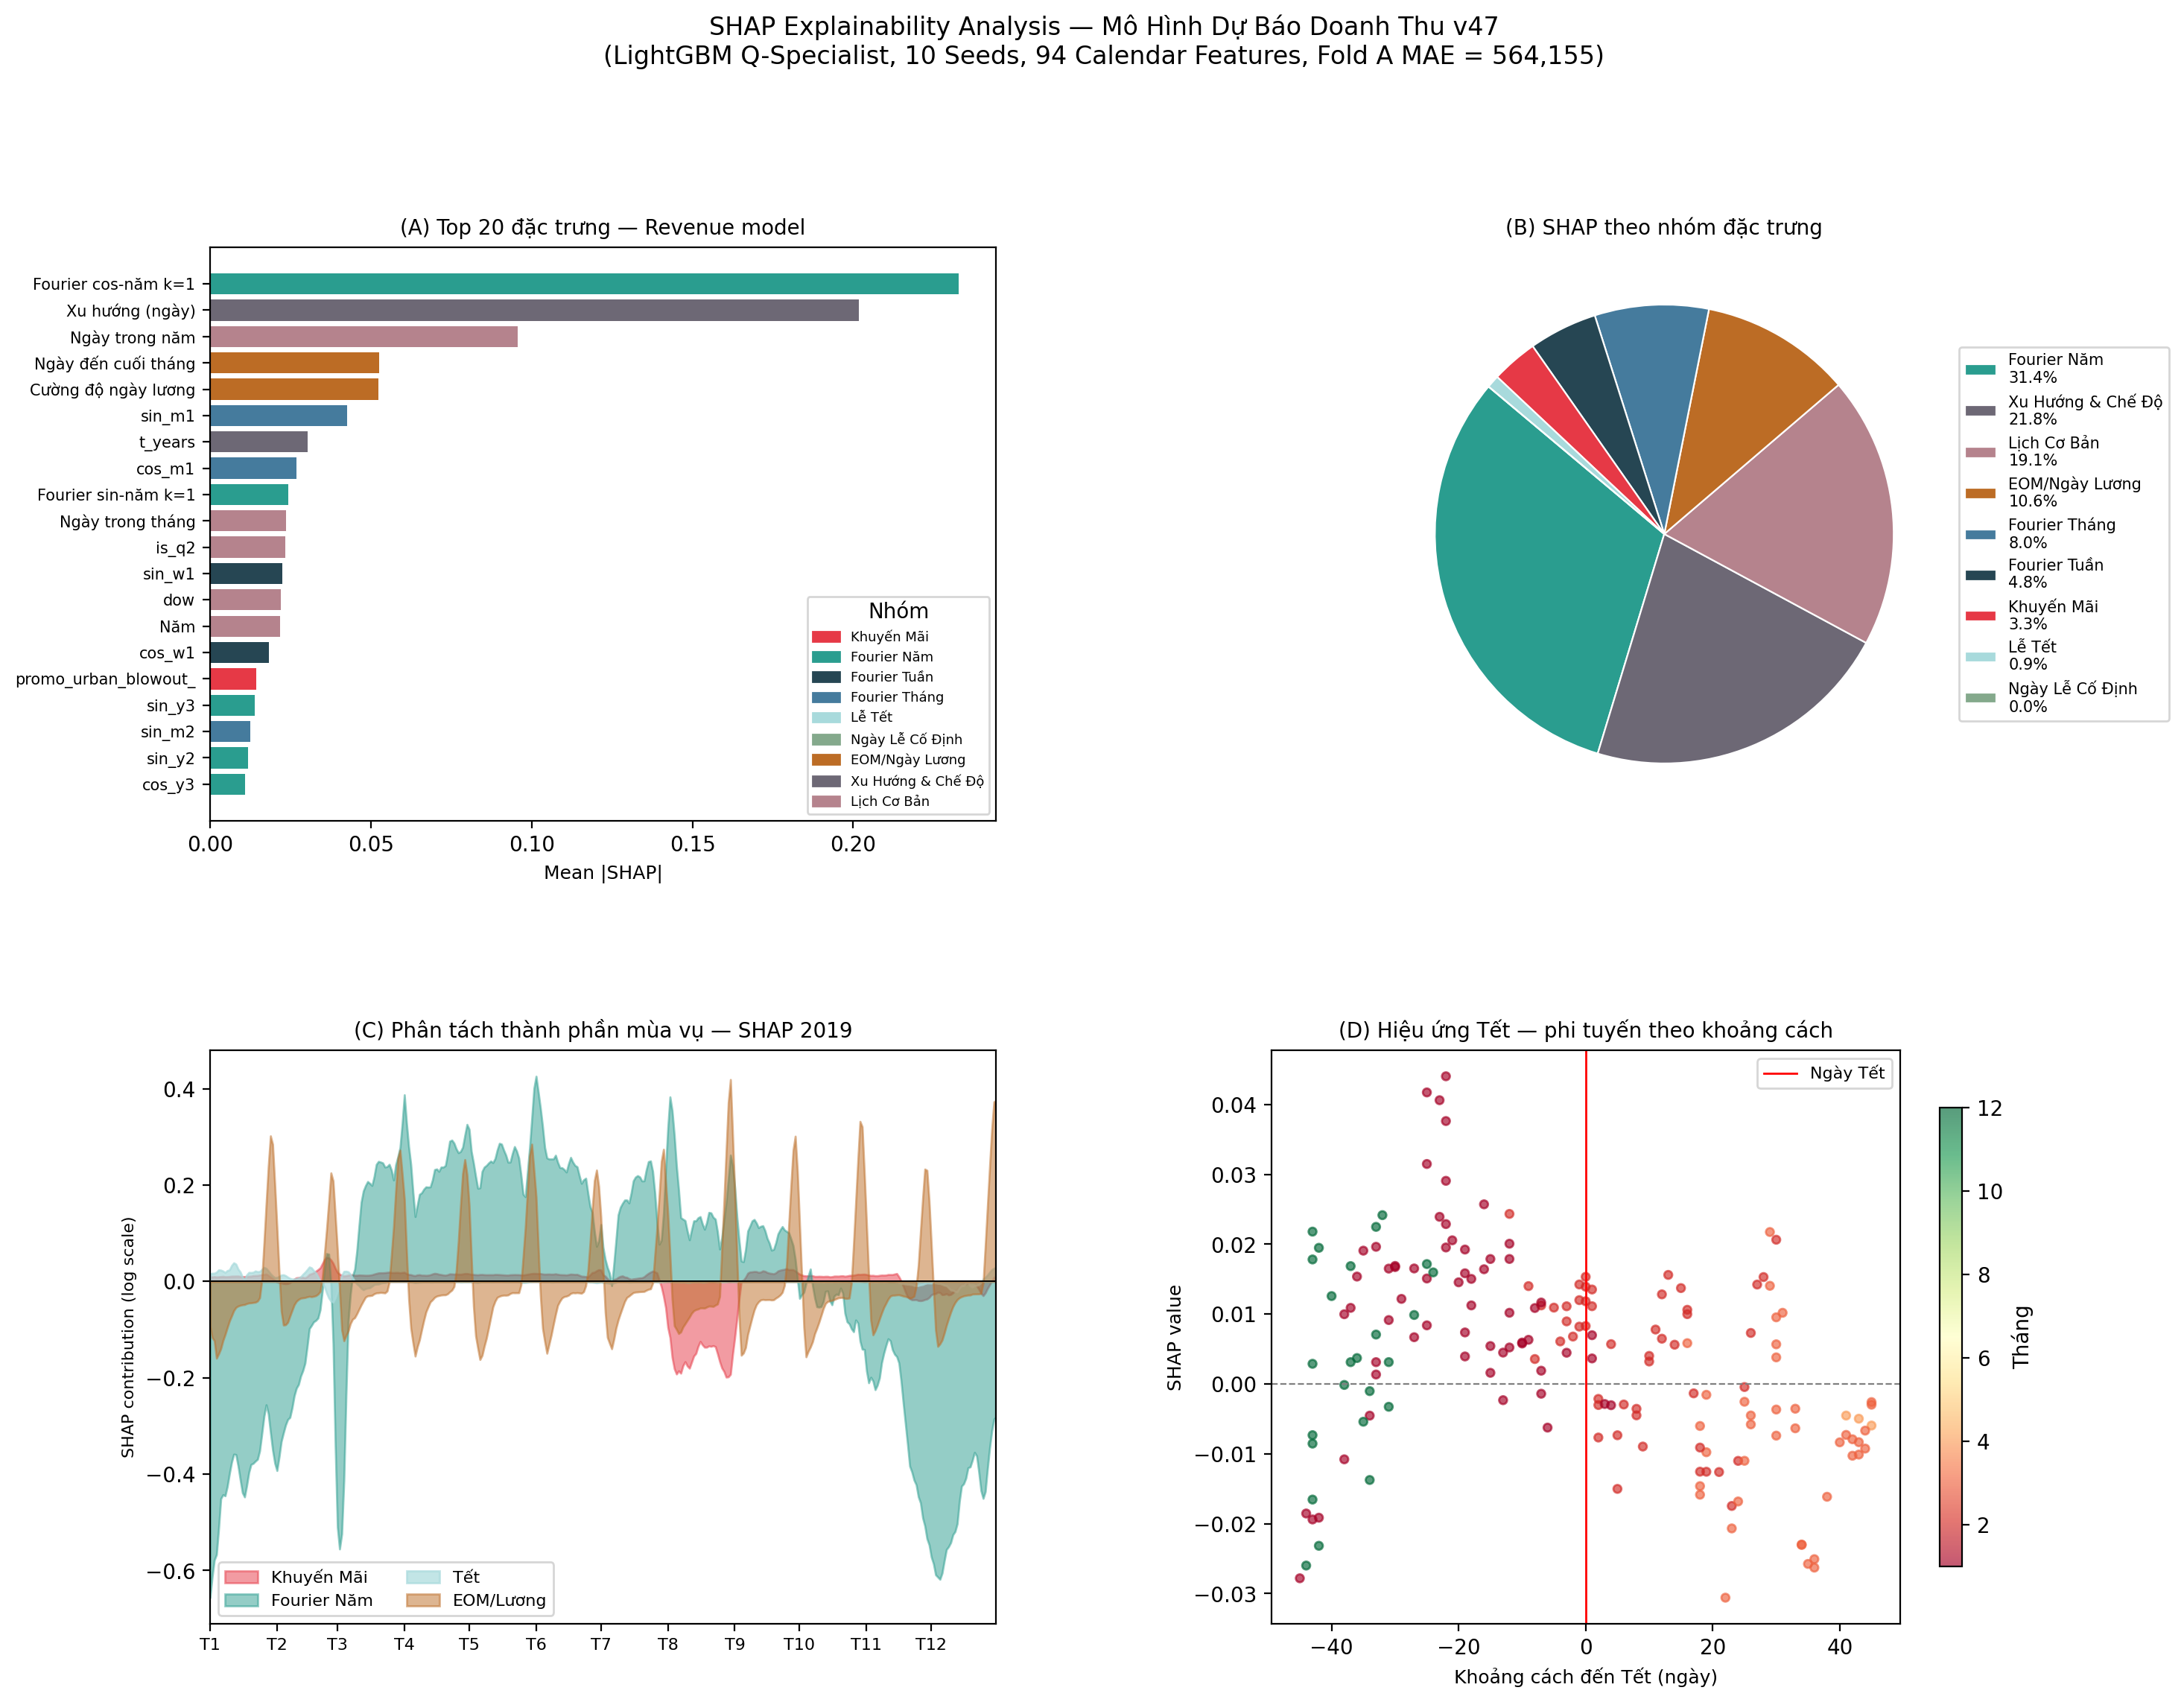
\includegraphics[width=0.97\linewidth]{figures/shap/shap_combined_report_figure.png}
\caption{\textbf{SHAP 4-Panel.} (A)~Top~20 features: cos\_y1 và t\_days dẫn đầu (|SHAP|$\approx$0,22 và 0,20). (B)~Phân bổ nhóm: Fourier Năm 31,5\%, Xu Hướng \& Chế Độ 21,9\%. (C)~Phân tách mùa vụ 2019: EOM/Lương spike ±0,3–0,5/tháng — lớn hơn Tết. (D)~Tết phi tuyến: dương $-$14 đến $-$3 ngày, âm ngay ngày Tết và $+$1 đến $+$4 ngày.}
\label{fig:shap_main}
\end{figure}

\textbf{Diễn giải bằng ngôn ngữ kinh doanh} (xem chi tiết SHAP tại Phụ lục~D):
\begin{itemize}
  \item \textbf{Mùa vụ (31,5\%):} T4–T6 đỉnh tự nhiên (cos\_y1 $\to$ SHAP $+0,3$); T11–T12 đáy ($-0,6$) nếu không có Year-End Sale. Cần kế hoạch nhân sự và tồn kho theo chu kỳ 2,6×.
  \item \textbf{Xu hướng \& Chế độ (21,9\%):} t\_days phân biệt đúng 3 era (SHAP 2017=$+0,22$, 2021=$-0,40$). Đây là lý do CR\_FLAT = 1,2649 cần thiết — bù gap giữa mức 2022 và mức phục hồi 2023–2024.
  \item \textbf{Ngày lương (10,7\%):} payday\_intensity=1,0 (ngày 29–31) $\to$ SHAP $+0,2$–$0,35$ nhất quán mọi quý, mạnh hơn nhiều ngày lễ. \textit{Hành động:} flash sale ngày 28–31.
  \item \textbf{Urban Blowout — Promo Paradox:} LGB gain importance = 48,7\% splits nhưng SHAP promo = 3,3\%. Không mâu thuẫn: promo active chỉ 8\% số ngày. Seasonal decomp (Phụ lục~D) cho thấy Urban Blowout tạo SHAP \textit{âm} — mô hình nhận diện đúng event margin-negative, biện hộ cho CC per-segment.
\end{itemize}

\textbf{Revenue vs COGS:} cùng top-2 features, nhưng COGS nhạy cảm hơn với sin\_y1 (pha lệch 90°) — chi phí và doanh thu không cùng pha, biện hộ cho 2 mô hình riêng biệt (Hình~\ref{fig:cogs_rev_shap}, Phụ lục~D).

% ===================================================================
\section{Kết Luận}
% ===================================================================

\vspace{-2pt}
Pipeline 29 phiên bản với mọi tham số có nguồn gốc thực nghiệm rõ ràng. Hai đóng góp chính: (1)~tách biệt \textit{shape learning} (LGB + calendar features) và \textit{level correction} (CR từ YoY sector growth); (2)~CC per-segment xử lý đúng Q3-odd margin âm. SHAP xác nhận mô hình học đúng 3 thành phần: mùa vụ Fourier, dịch chuyển era, chu kỳ ngày lương. LB = 669.087 (best) chứng minh calendar features + kinh tế học ngành outperform N-HiTS (686.351) trong bối cảnh structural break dài hạn. GitHub: \url{https://github.com/inwinnieworld/DatathonTop}.

% ===================================================================
\section*{Tài Liệu Tham Khảo}
% ===================================================================
\small
\begin{enumerate}[label={[\arabic*]},leftmargin=*,noitemsep,topsep=2pt]
  \item Ke, G. et al. (2017). LightGBM: A Highly Efficient Gradient Boosting Decision Tree. \textit{NeurIPS}.
  \item Taylor, S.J. \& Letham, B. (2018). Forecasting at scale. \textit{The American Statistician}, 72(1), 37–45.
  \item Lundberg, S.M. \& Lee, S.-I. (2017). A Unified Approach to Interpreting Model Predictions. \textit{NeurIPS}.
  \item Bộ Công Thương Việt Nam / MoIT (2022). Báo cáo Thương mại điện tử Việt Nam 2022.
  \item Challu, C. et al. (2023). NHITS: Neural Hierarchical Interpolation for Time Series Forecasting. \textit{AAAI}.
\end{enumerate}

% ===================================================================
% ██████  APPENDIX  ██████
% ===================================================================
\clearpage
\appendix

% ------------------------------------------------------------------
\clearpage
\section{Dashboard EDA Đầy Đủ}
% ------------------------------------------------------------------

\begin{figure}[htbp]
\centering
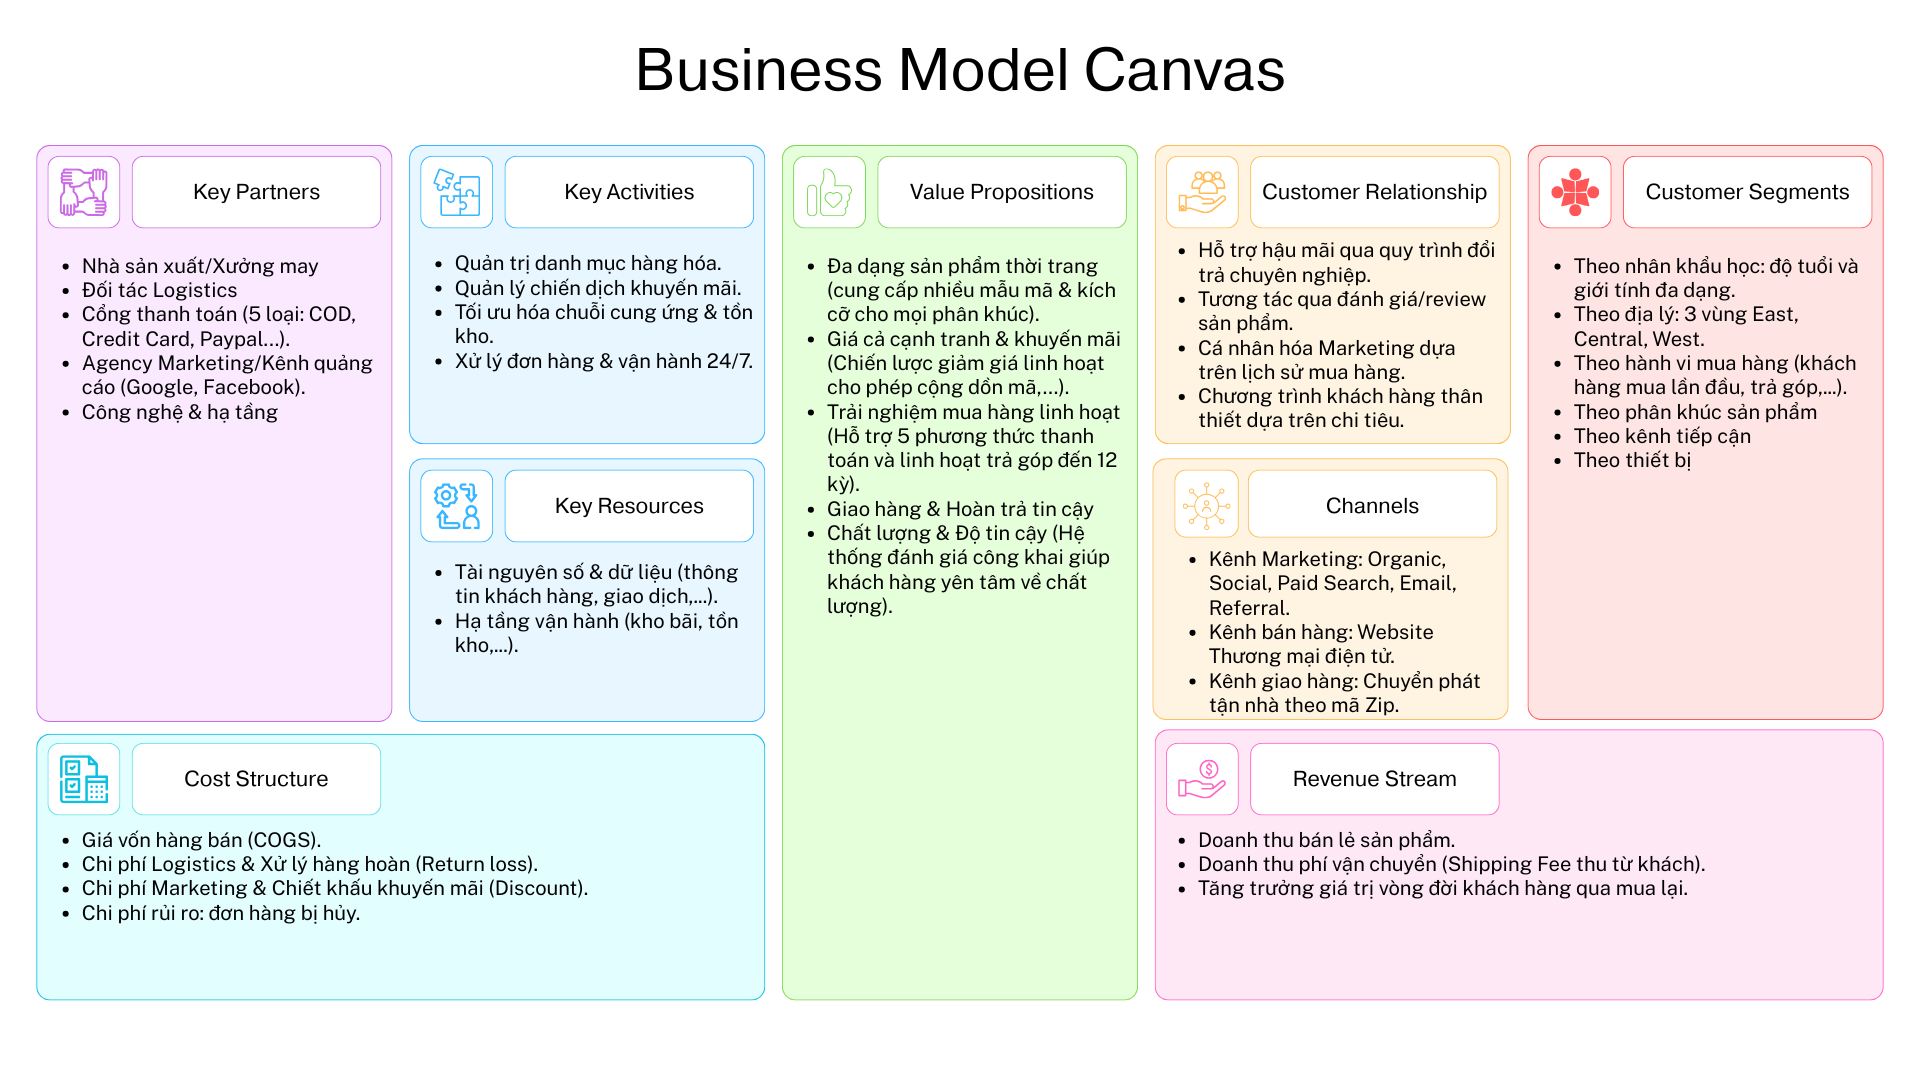
\includegraphics[width=0.42\linewidth]{figures/eda/Business_Model_Canvas.png}
\caption{Business Model Canvas — mô hình vận hành pure-play e-commerce thời trang VN.}
\label{fig:bmc}
\end{figure}

\begin{figure}[htbp]
\centering
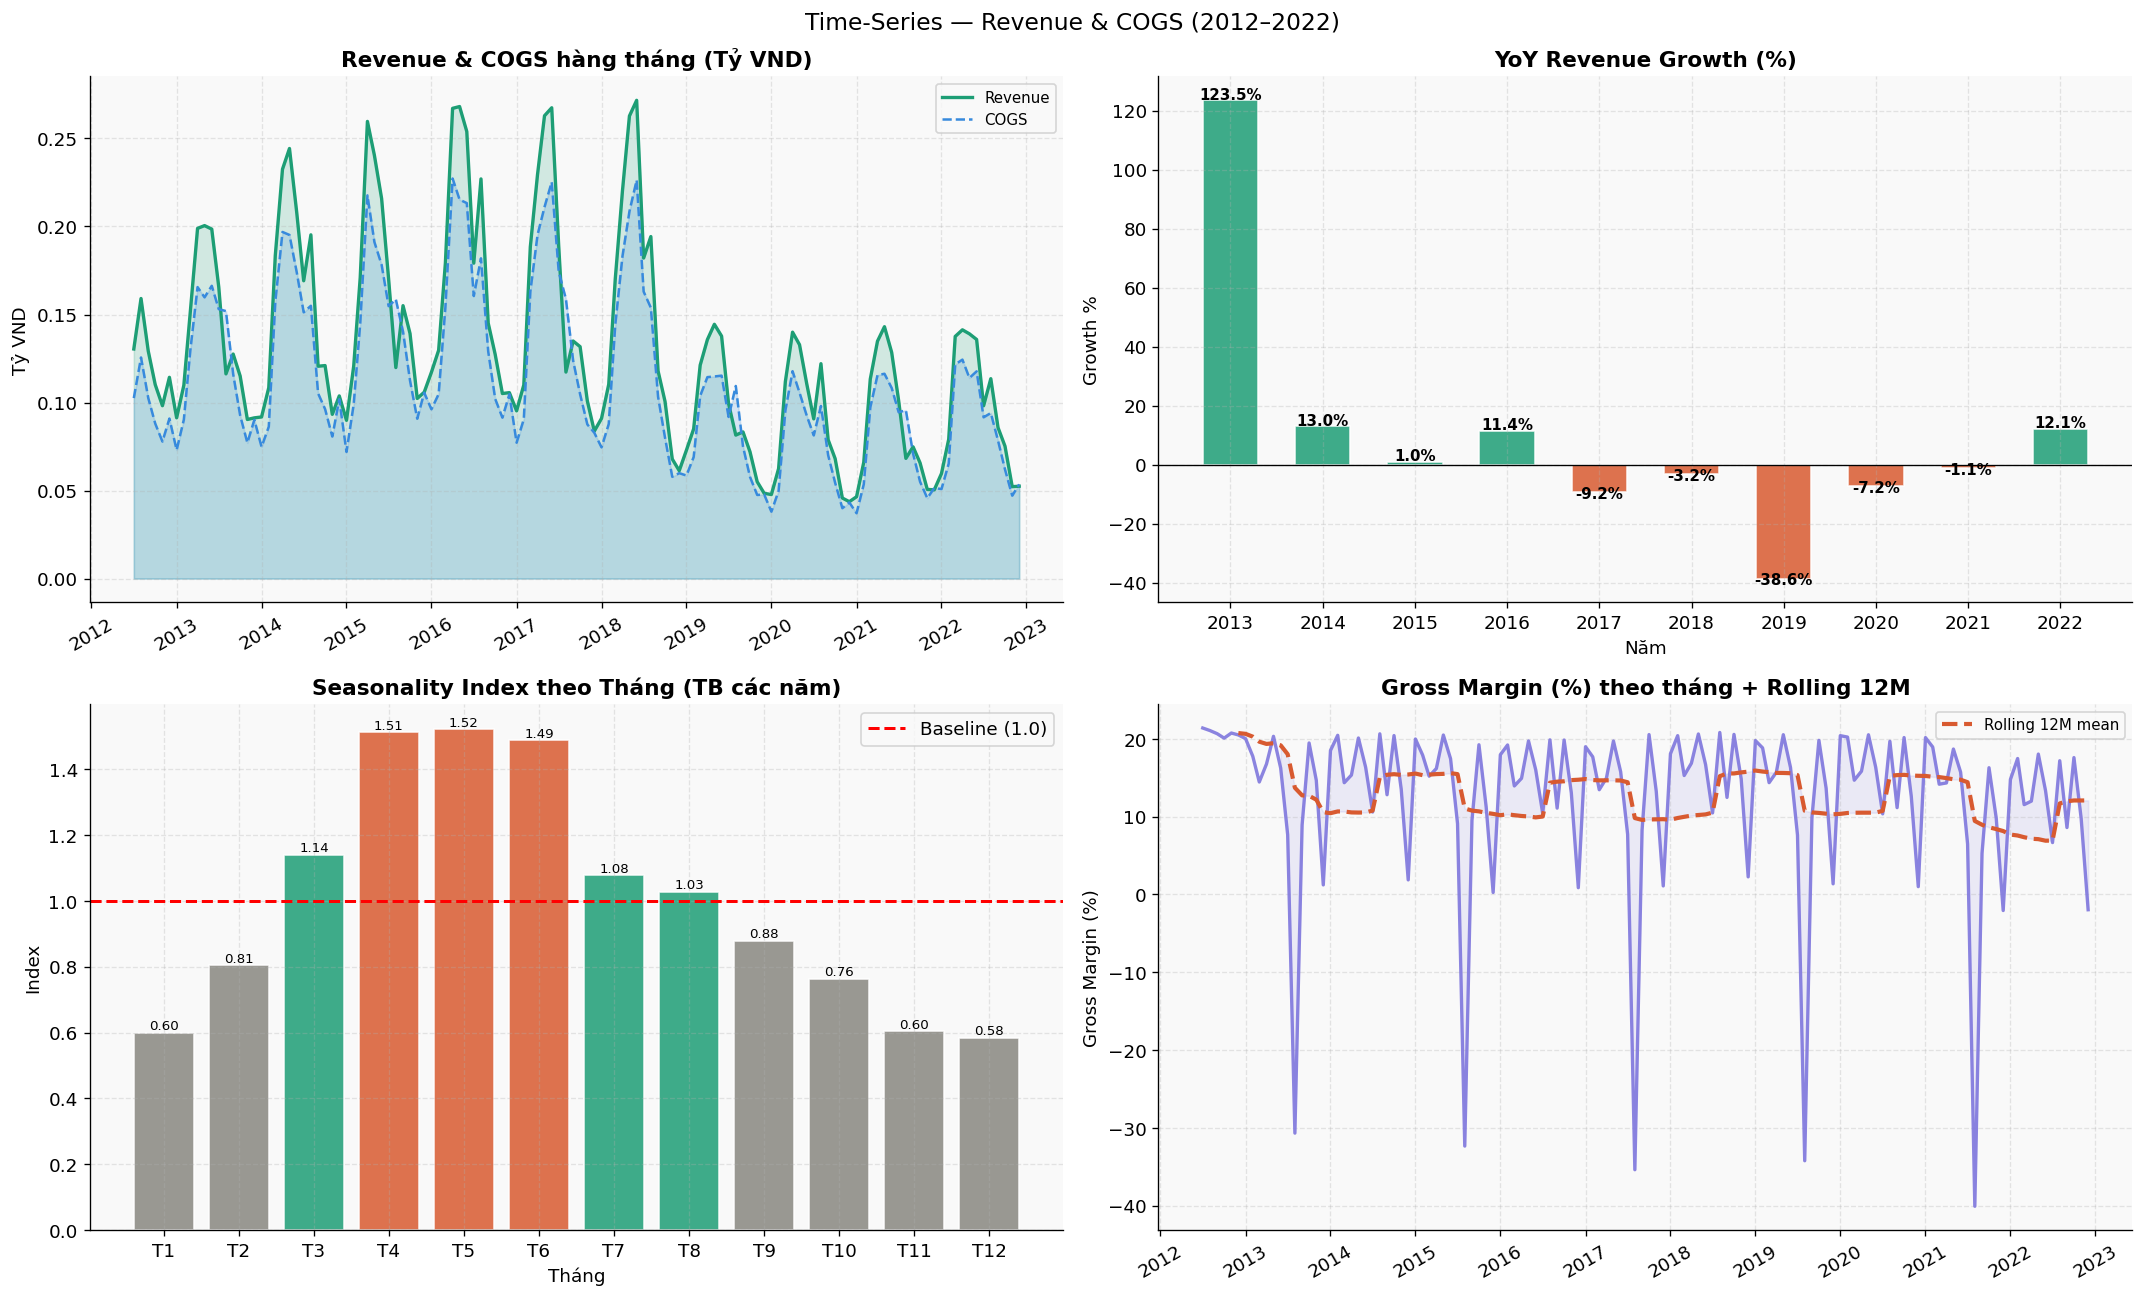
\includegraphics[width=\linewidth]{figures/eda/fig_timeseries_main.png}
\caption{\textbf{Chuỗi thời gian tổng hợp.} Trên-trái: Revenue \& COGS hàng tháng. Trên-phải: YoY — sụt $-38,6\%$ (2019) và phục hồi $+12,1\%$ (2022). Dưới-trái: Seasonality index đỉnh T4–T6 (1,49–1,52), đáy T11–T1 (0,58–0,60), biên độ 2,6×. Dưới-phải: Gross margin rolling 12M xu hướng giảm từ 2016–2022.}
\label{fig:ts_main}
\end{figure}

\begin{figure}[htbp]
\centering
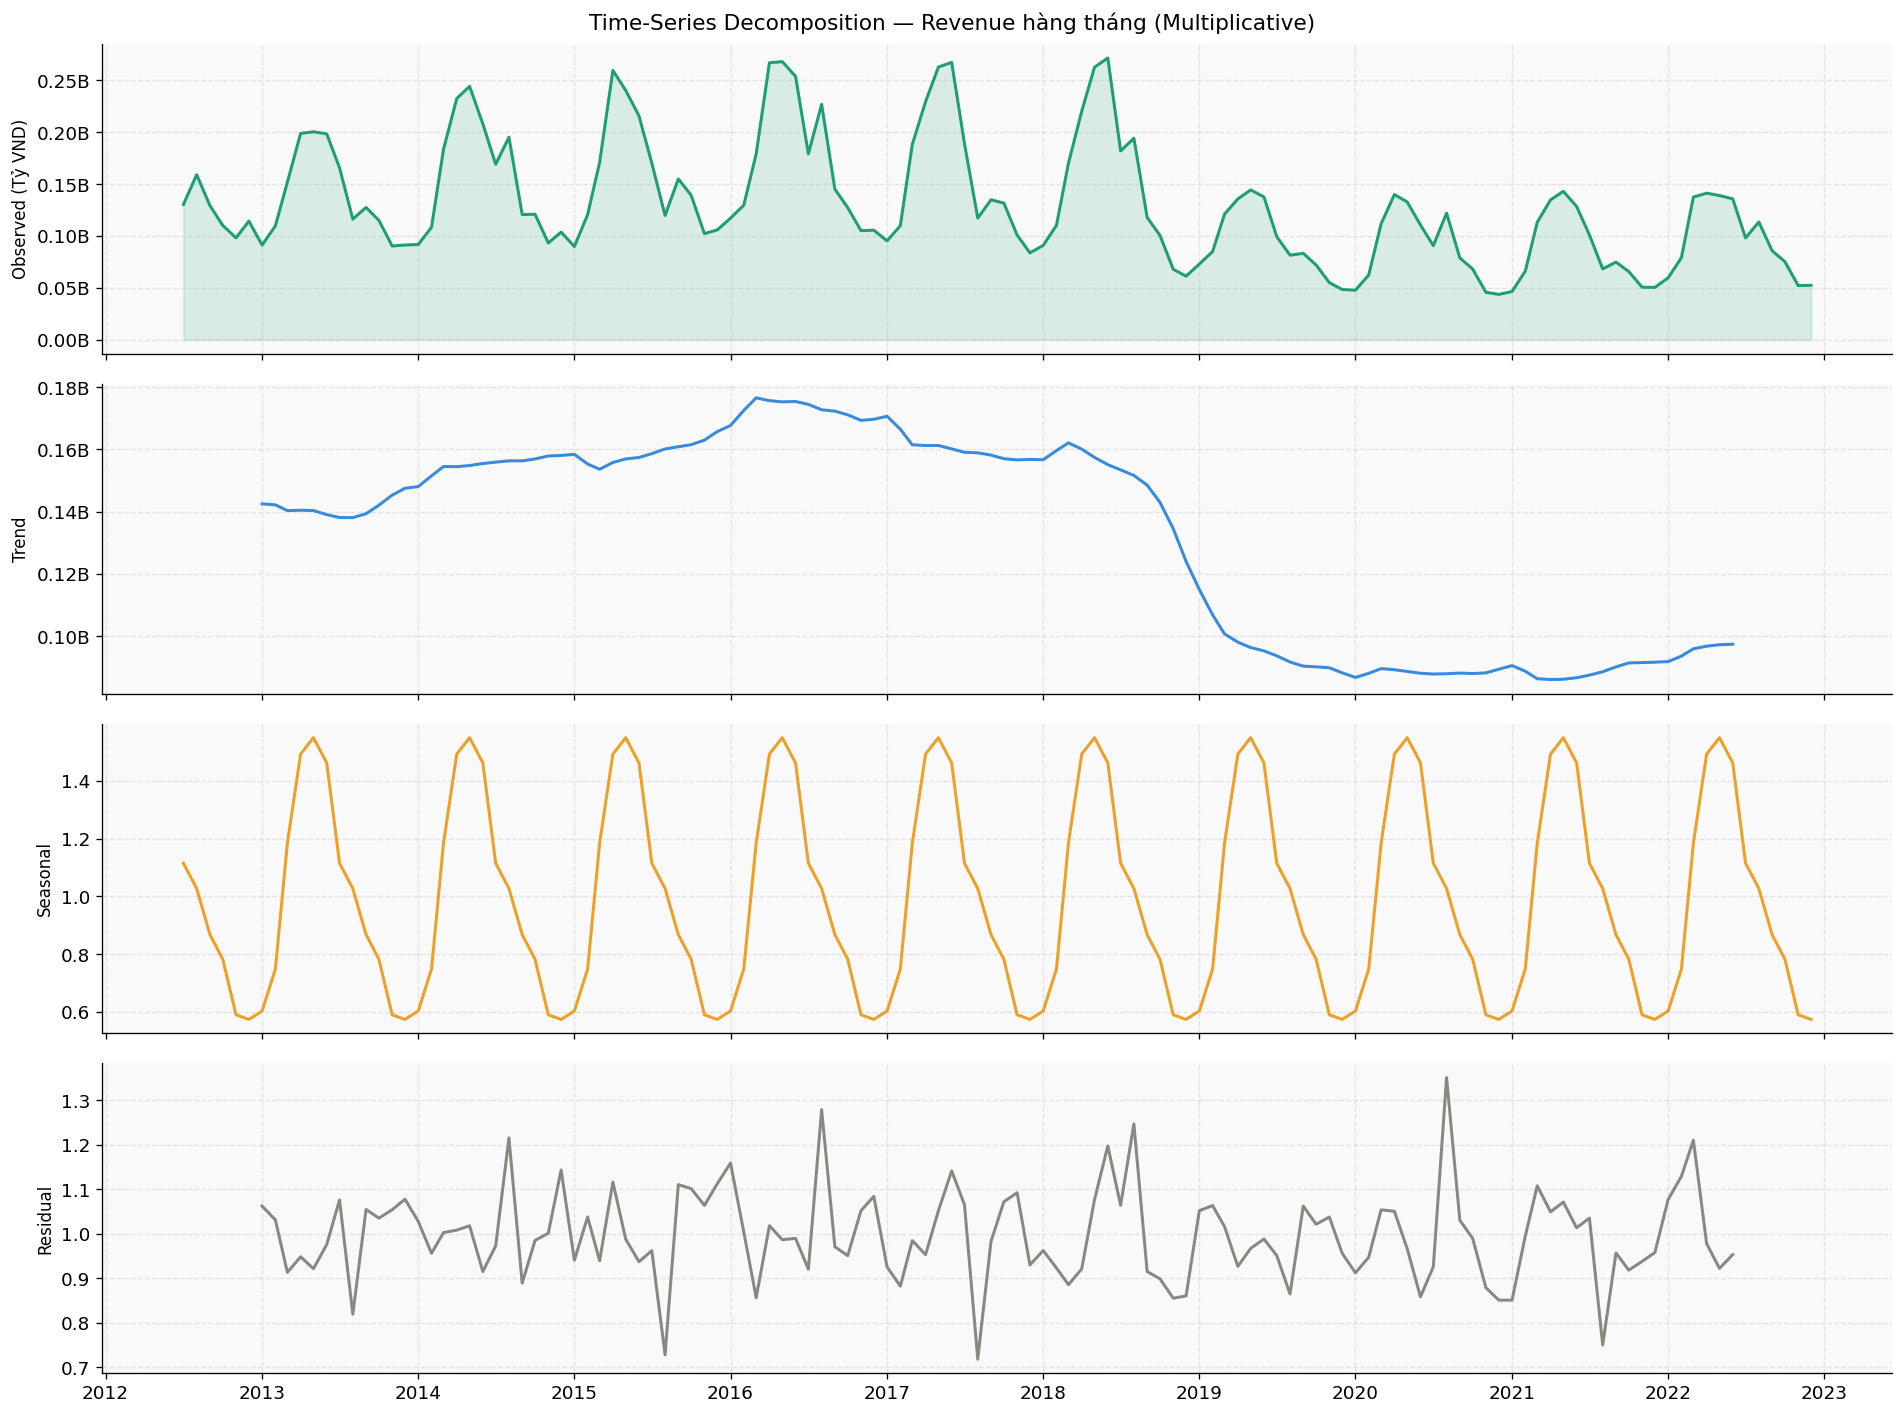
\includegraphics[width=\linewidth]{figures/eda/fig_decompose.png}
\caption{\textbf{Phân tách Multiplicative.} Trend giảm đột ngột 2019, Seasonal ổn định — level thay đổi, shape không đổi. Residual 2021 spike 1,3× do lockdown.}
\label{fig:decompose}
\end{figure}

\begin{figure}[htbp]
\centering
\begin{subfigure}[b]{0.49\linewidth}
  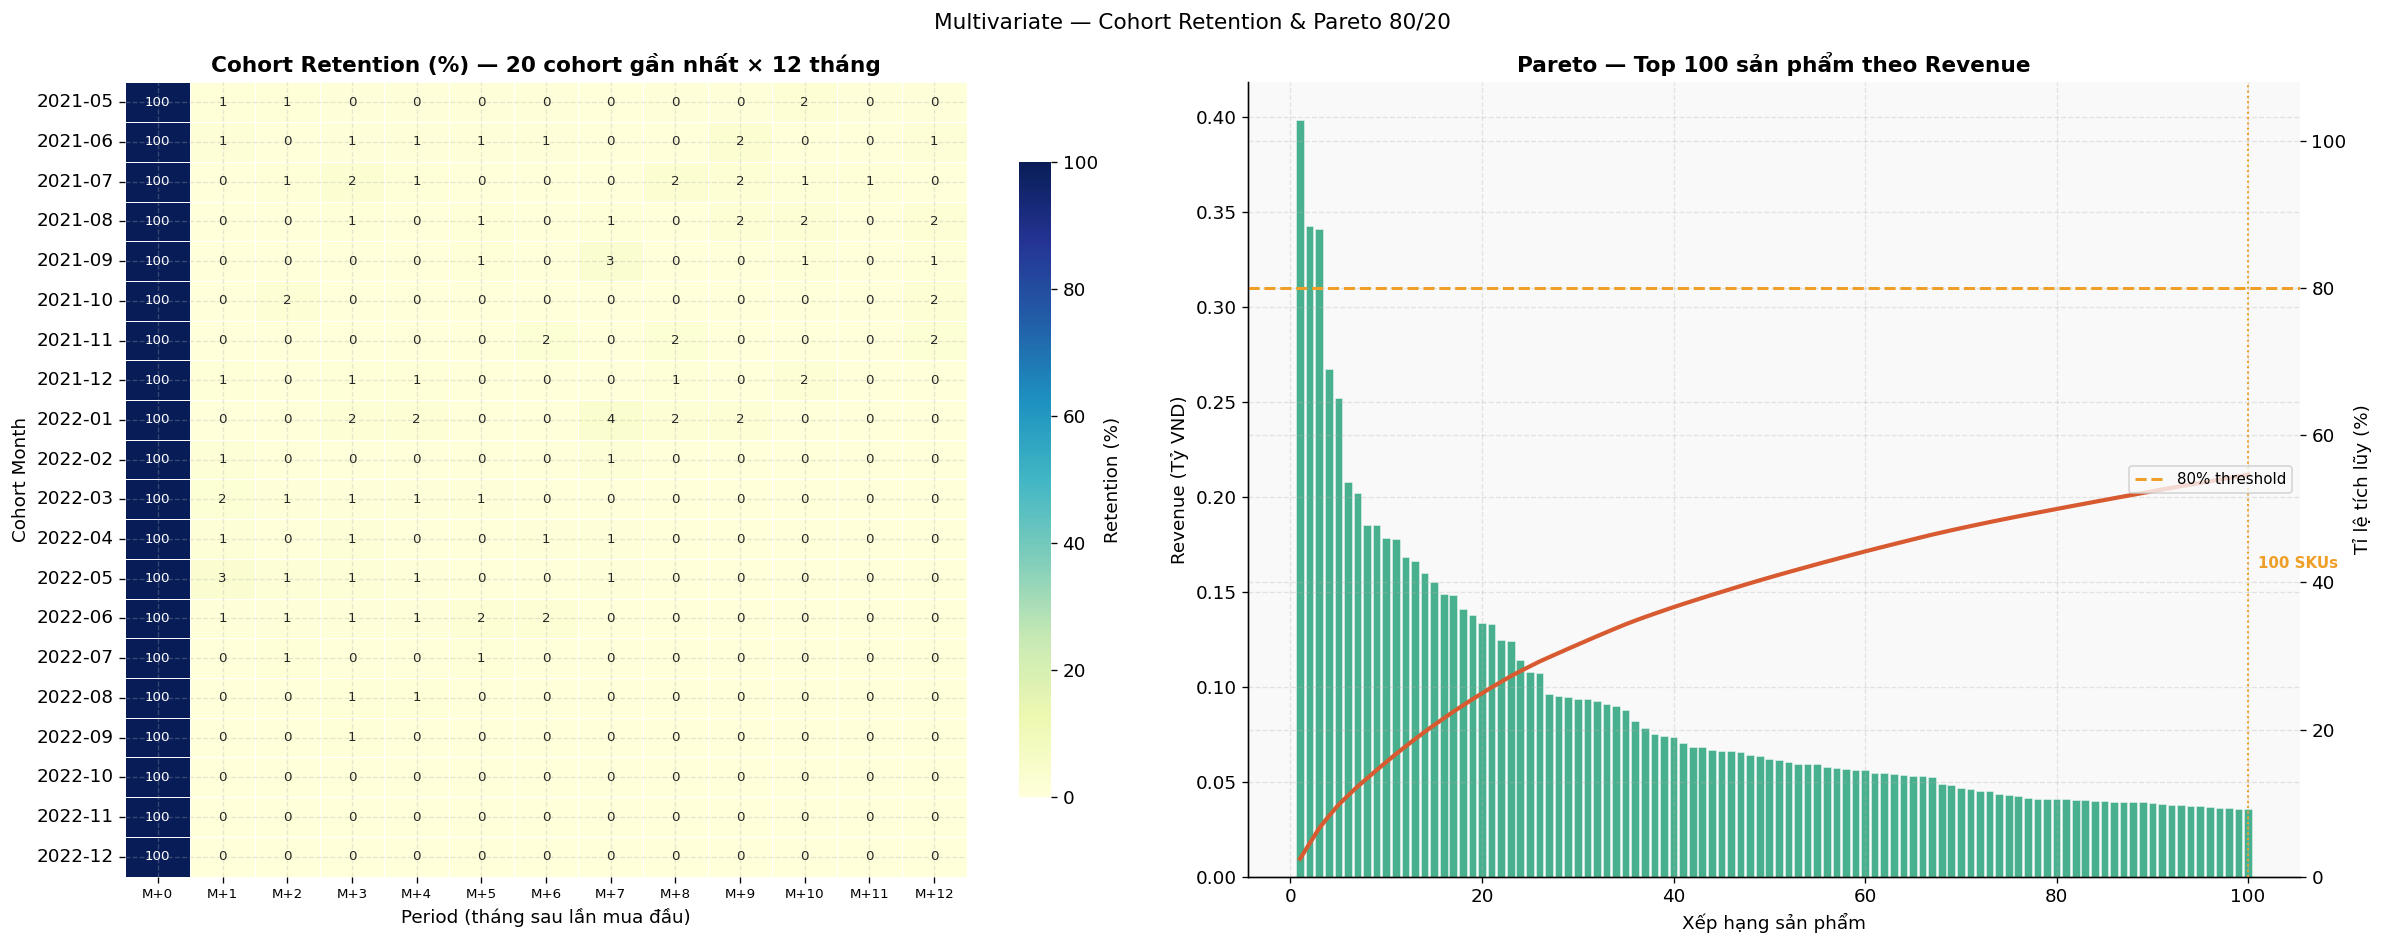
\includegraphics[width=\linewidth]{figures/eda/fig_multi_cohort_pareto.png}
  \caption{Cohort retention $\approx$0\% sau M+1; Pareto top-20 SKU = 80\% revenue}
  \label{fig:cohort}
\end{subfigure}
\hfill
\begin{subfigure}[b]{0.49\linewidth}
  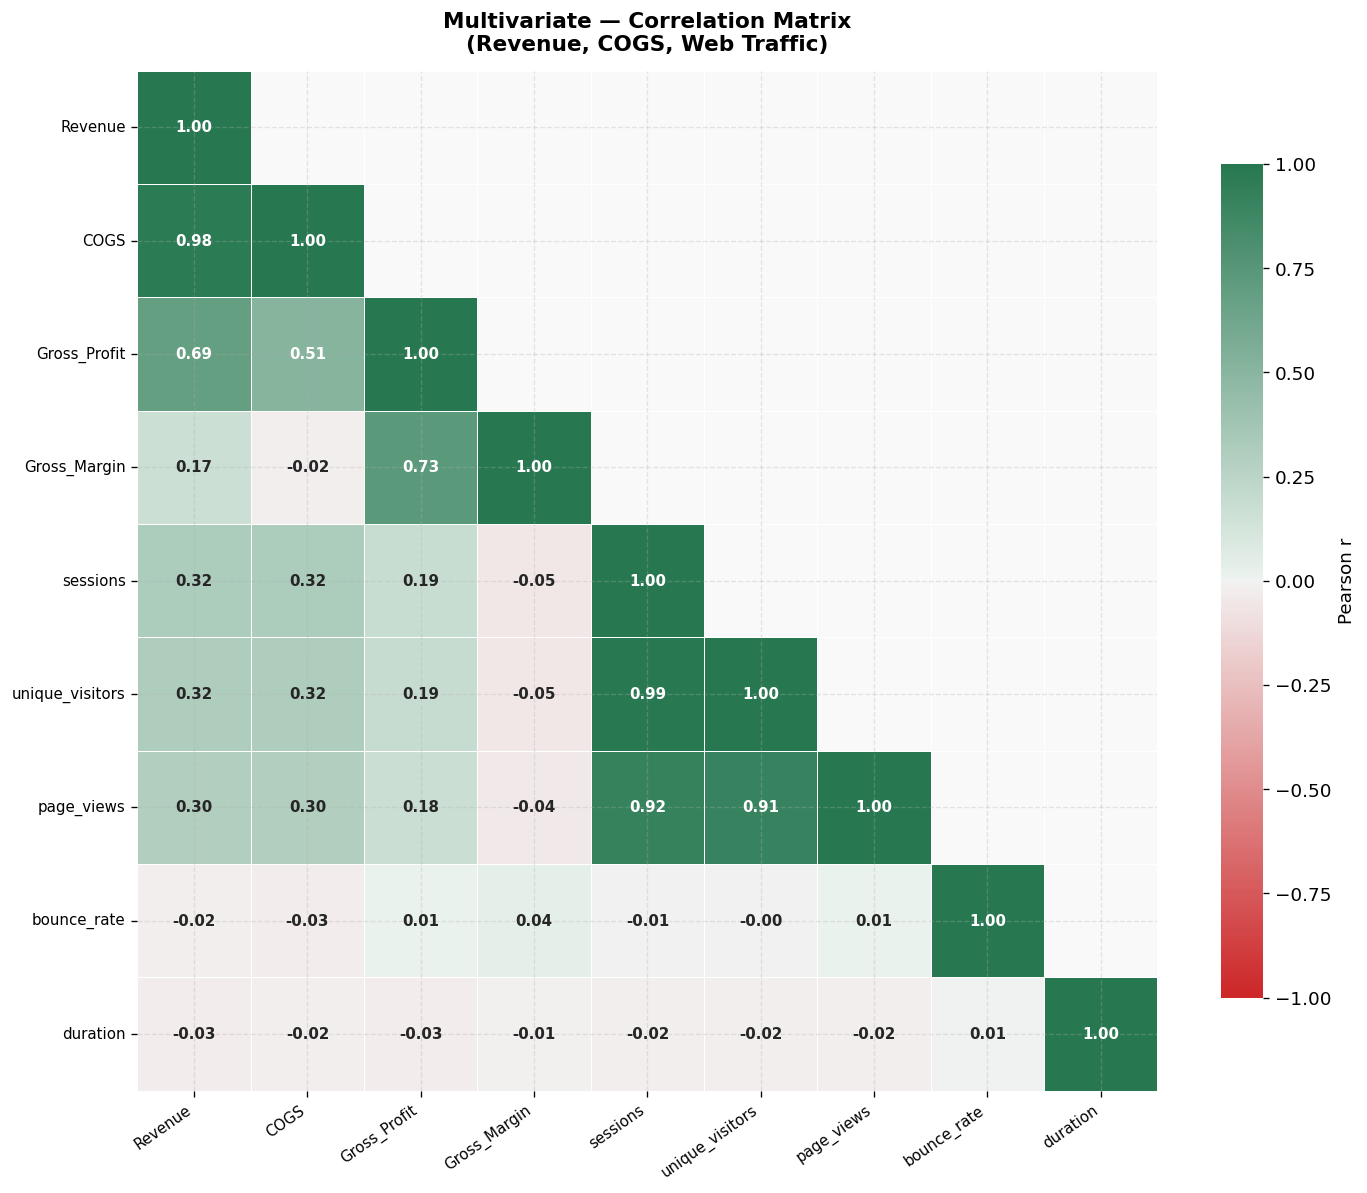
\includegraphics[width=\linewidth]{figures/eda/fig_multi_corr.png}
  \caption{Tương quan: Revenue–COGS $r=0,98$; Sessions–Revenue $r=0,32$; Bounce Rate $r=-0,02$}
  \label{fig:corr}
\end{subfigure}
\caption{Cohort Retention \& Ma trận Tương quan.}
\end{figure}

\begin{figure}[htbp]
\centering
\begin{subfigure}[b]{0.49\linewidth}
  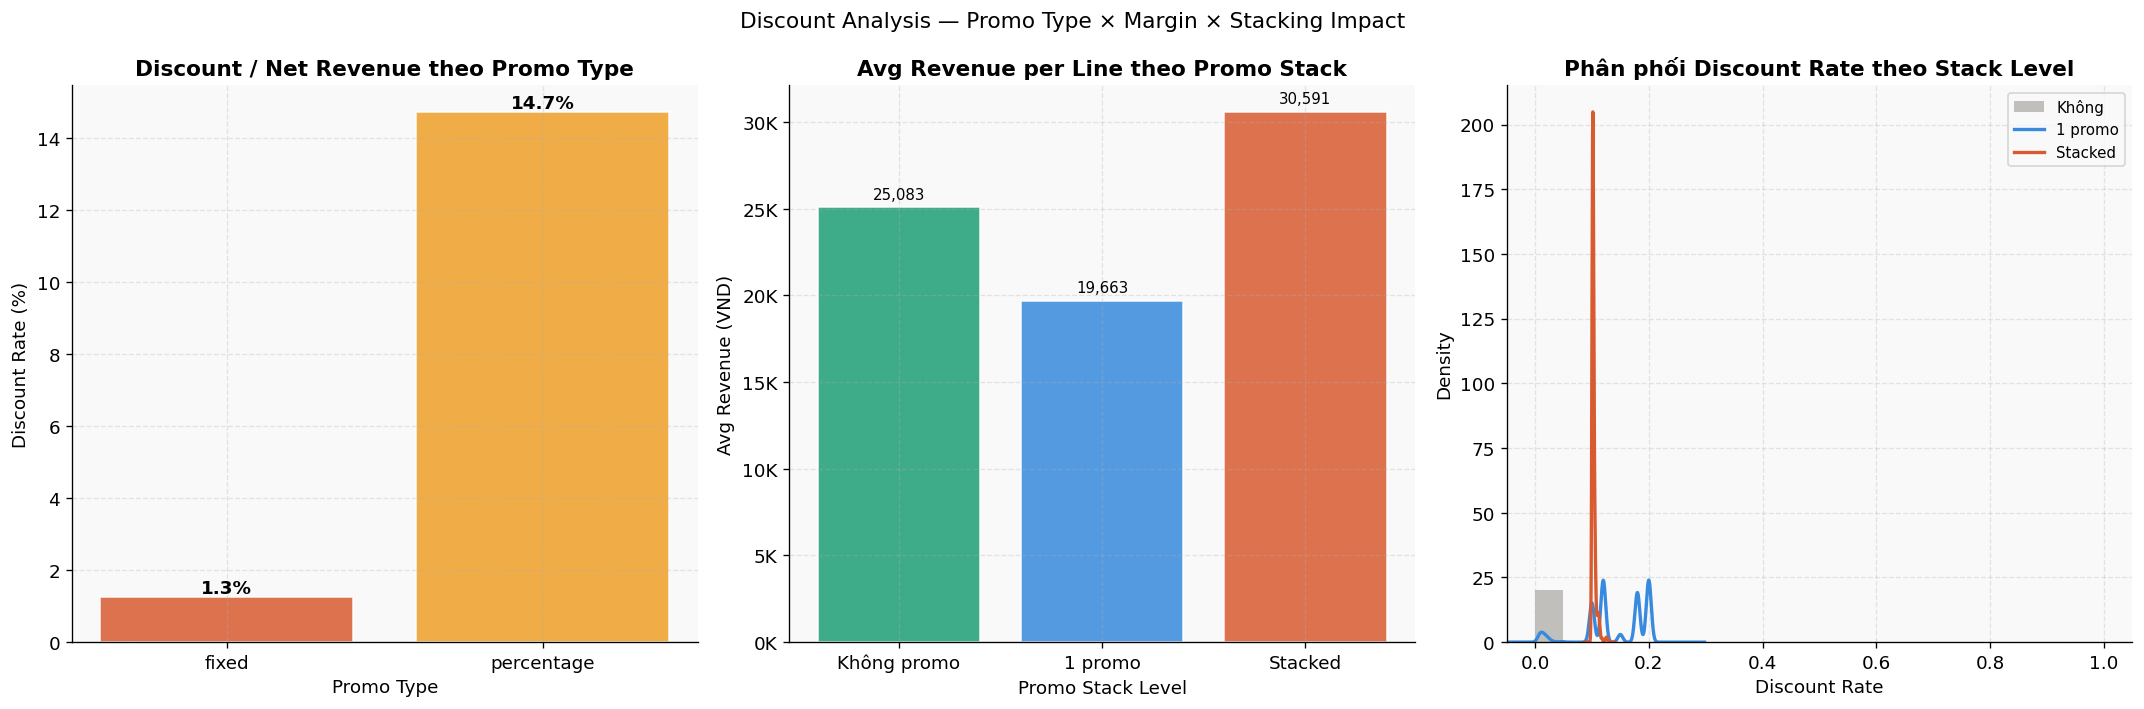
\includegraphics[width=\linewidth]{figures/eda/fig_discount_analysis.png}
  \caption{Discount: percentage-type = 14,7\% net rev; stacked orders có AOV cao nhất}
  \label{fig:discount}
\end{subfigure}
\hfill
\begin{subfigure}[b]{0.49\linewidth}
  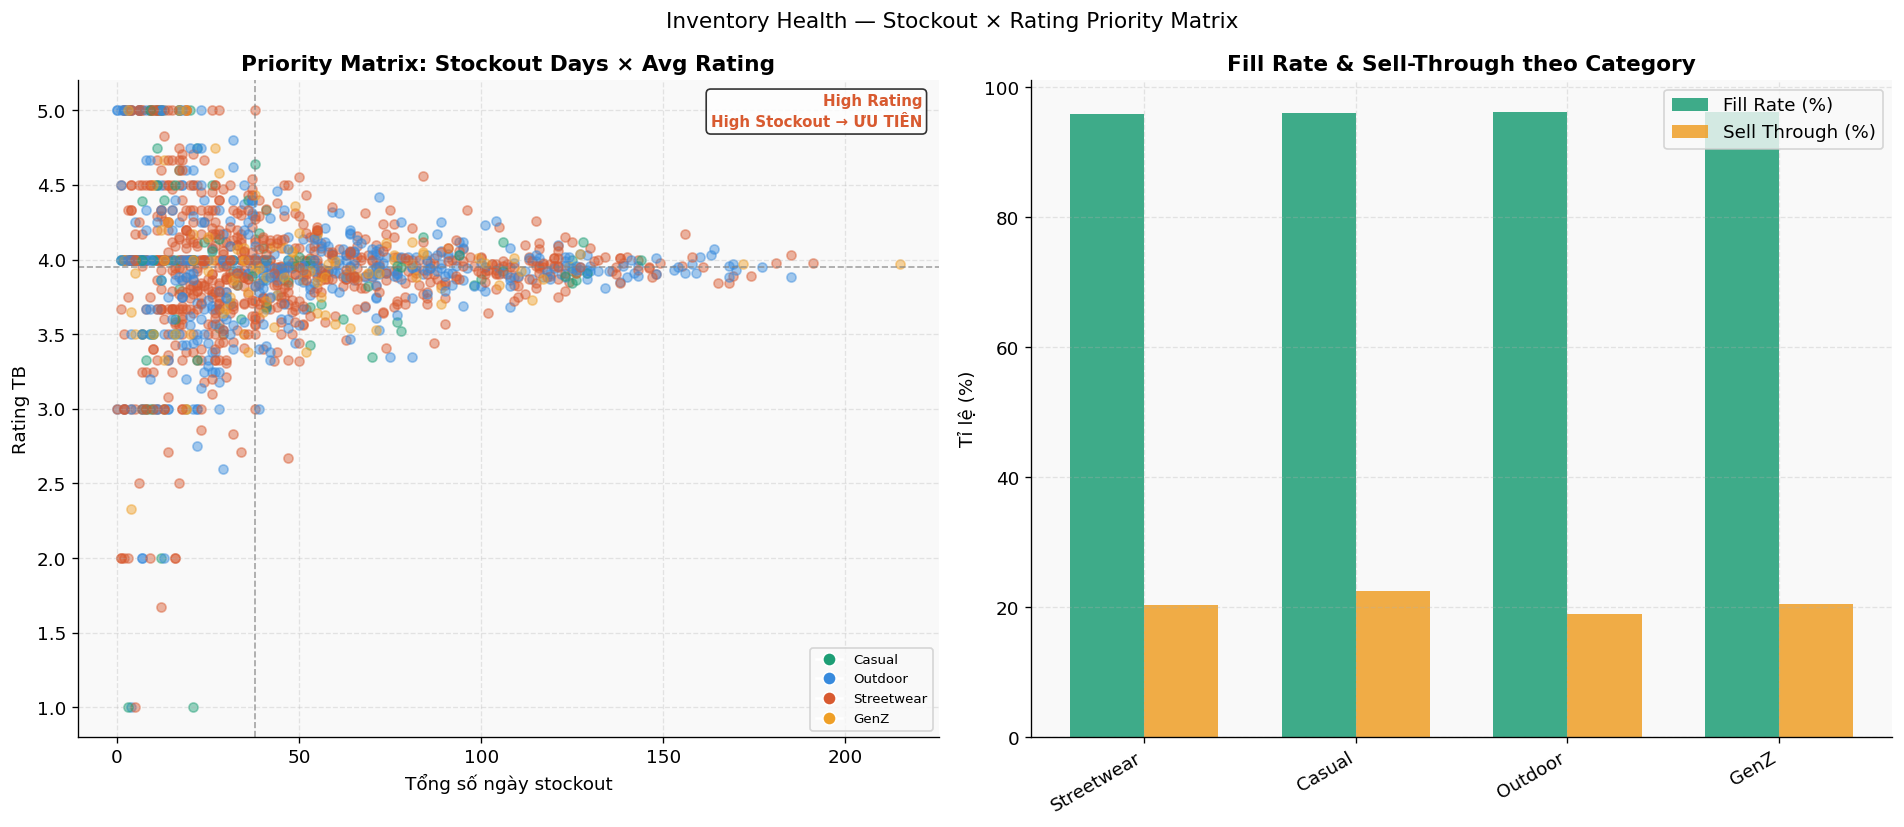
\includegraphics[width=\linewidth]{figures/eda/fig_inventory_health.png}
  \caption{Fill rate 95\% nhưng sell-through 20\%; SKU rating cao hay stockout nhất}
  \label{fig:inventory}
\end{subfigure}
\caption{Phân tích chiết khấu và sức khoẻ tồn kho.}
\end{figure}

\begin{figure}[htbp]
\centering
\begin{subfigure}[b]{0.49\linewidth}
  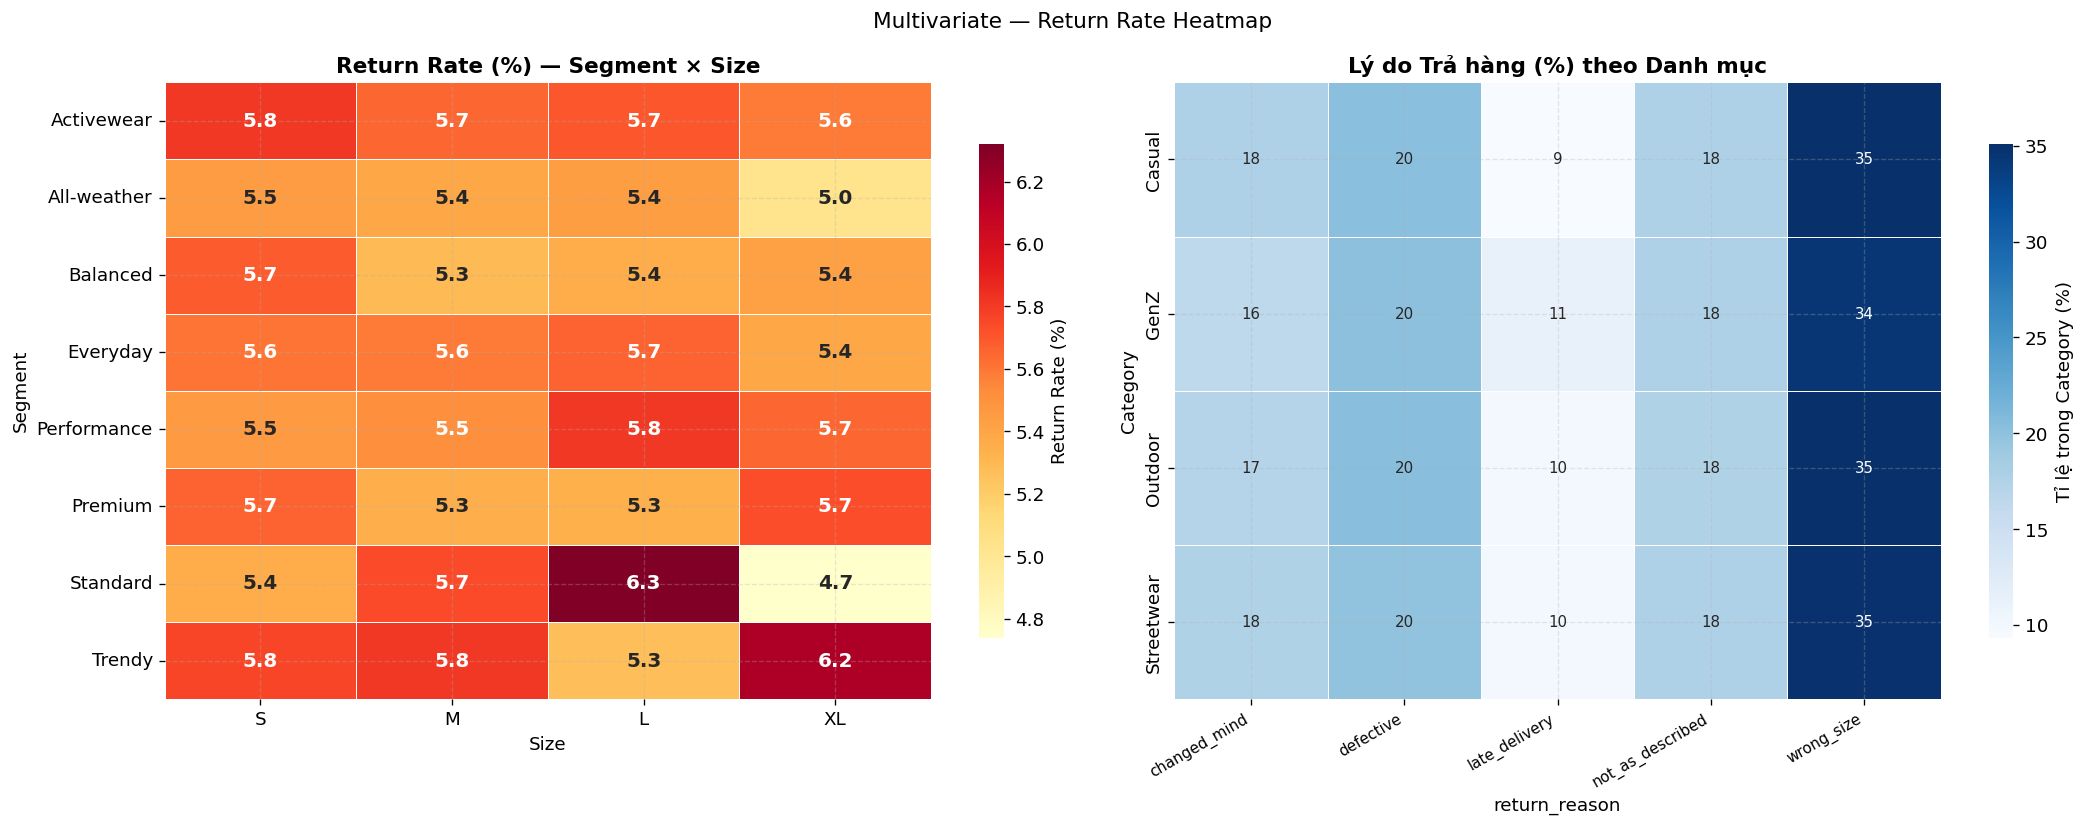
\includegraphics[width=\linewidth]{figures/eda/fig_multi_return_heatmap.png}
  \caption{Return heatmap: "wrong\_size" = 35\% nhất quán qua 4 danh mục}
  \label{fig:return_heatmap}
\end{subfigure}
\hfill
\begin{subfigure}[b]{0.49\linewidth}
  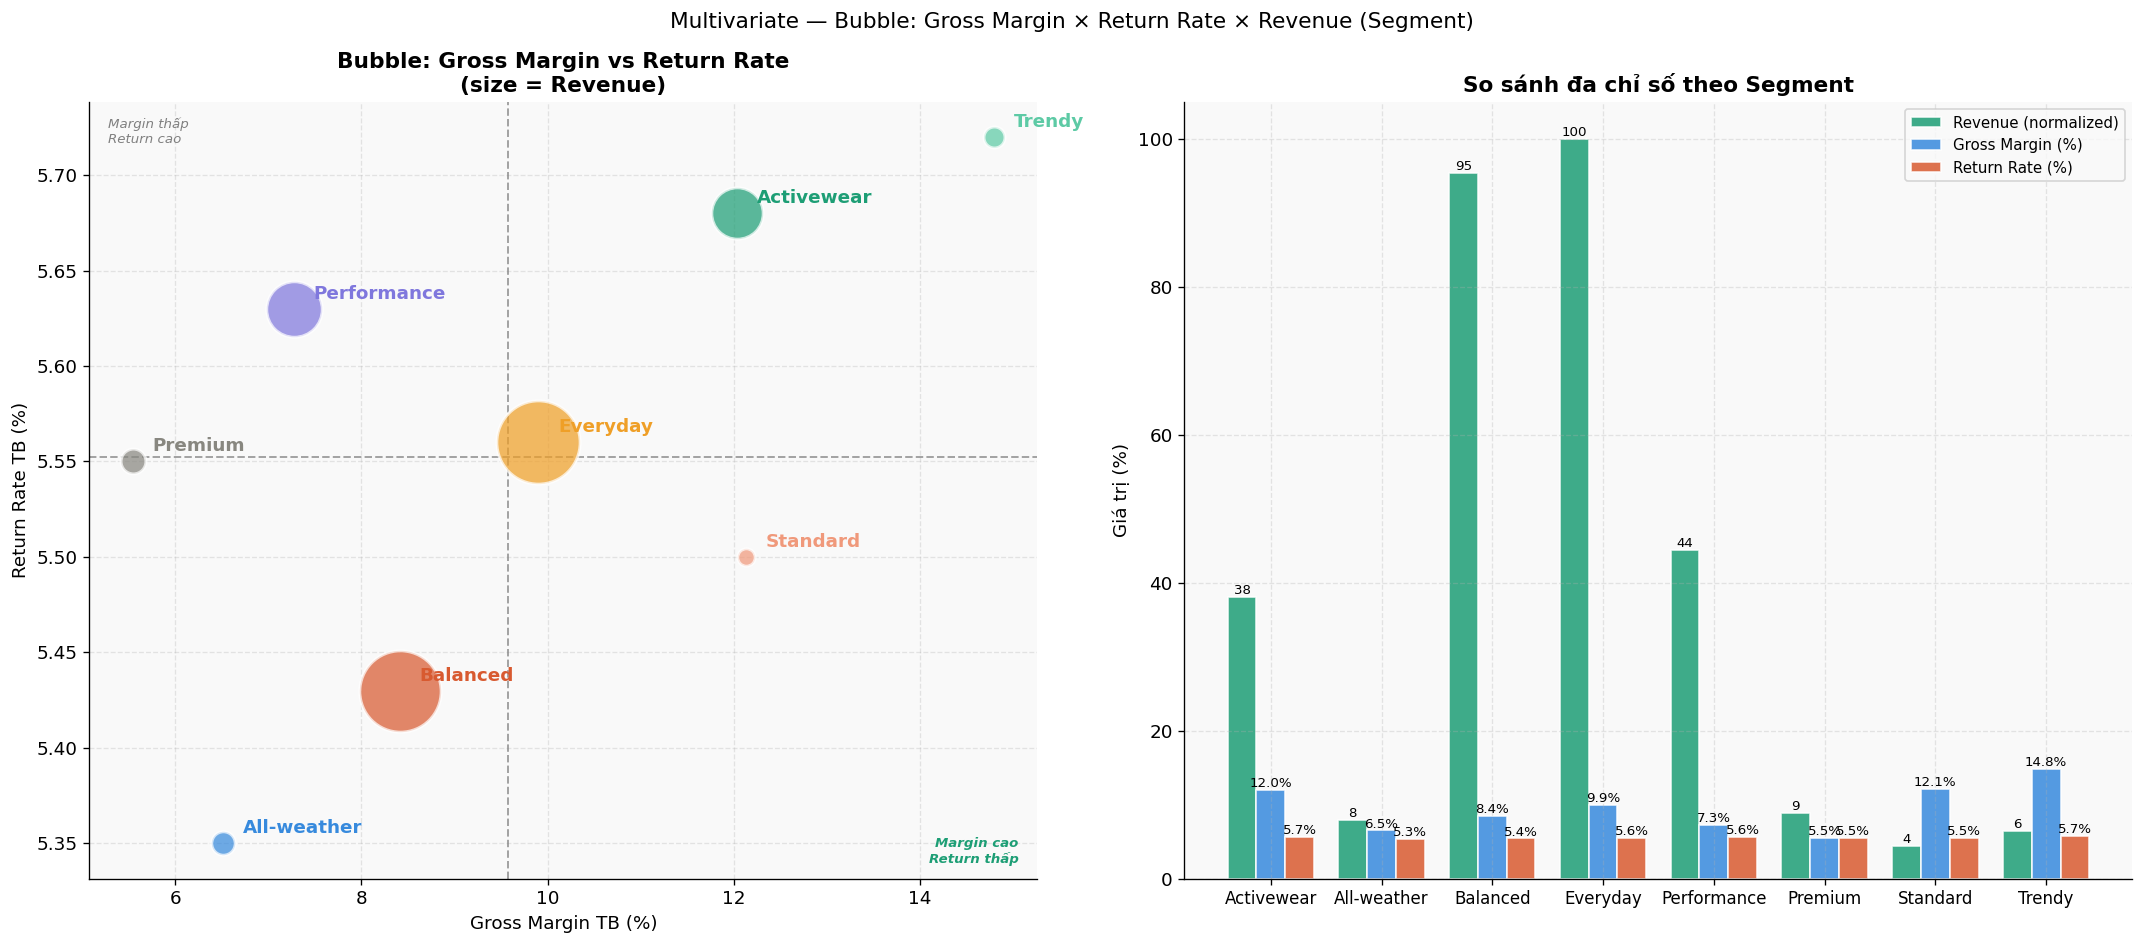
\includegraphics[width=\linewidth]{figures/eda/fig_multi_bubble.png}
  \caption{Bubble: Standard margin cao nhất (31,3\%), return thấp — segment tối ưu}
  \label{fig:bubble}
\end{subfigure}
\caption{Tỉ lệ trả hàng và phân tích đa chỉ số theo phân khúc.}
\end{figure}

\begin{figure}[htbp]
\centering
\begin{subfigure}[b]{0.49\linewidth}
  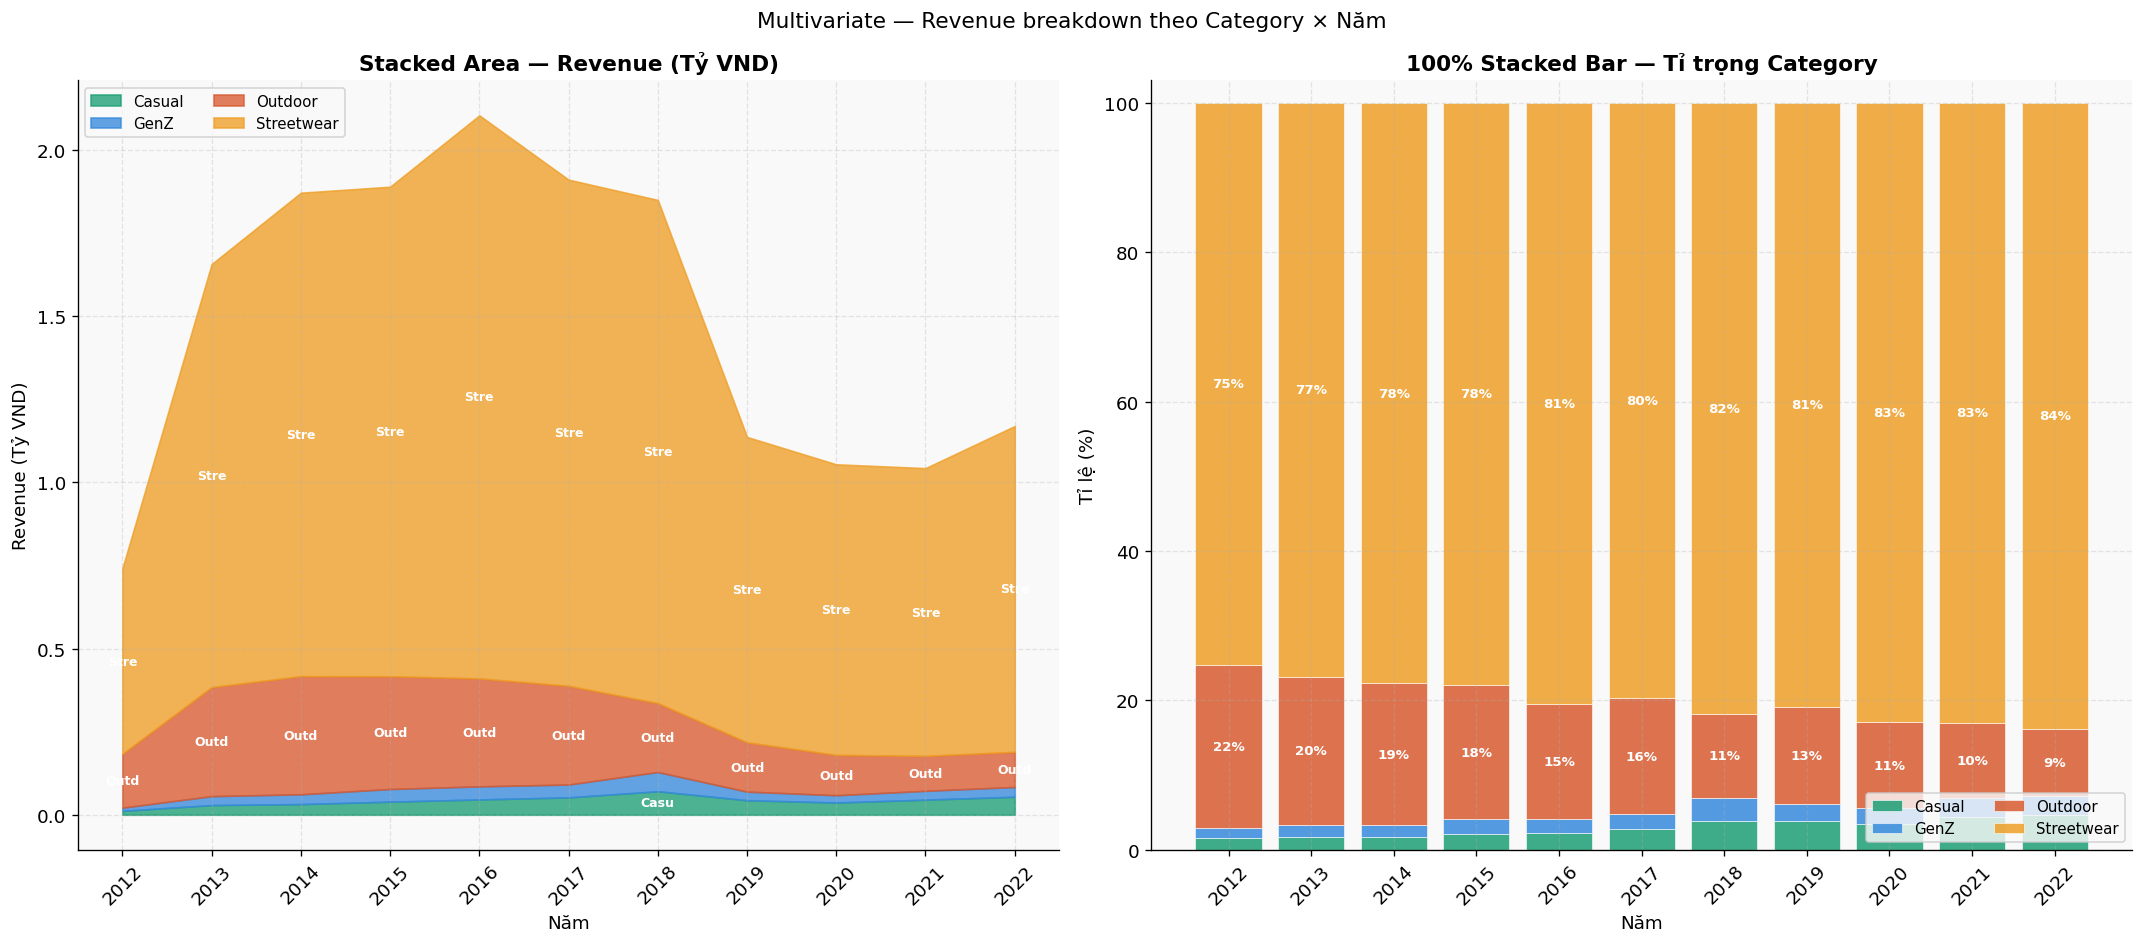
\includegraphics[width=\linewidth]{figures/eda/fig_multi_stacked.png}
  \caption{Streetwear 75\%$\to$84\% (2012–2022); Outdoor 22\%$\to$9\%}
  \label{fig:stacked}
\end{subfigure}
\hfill
\begin{subfigure}[b]{0.49\linewidth}
  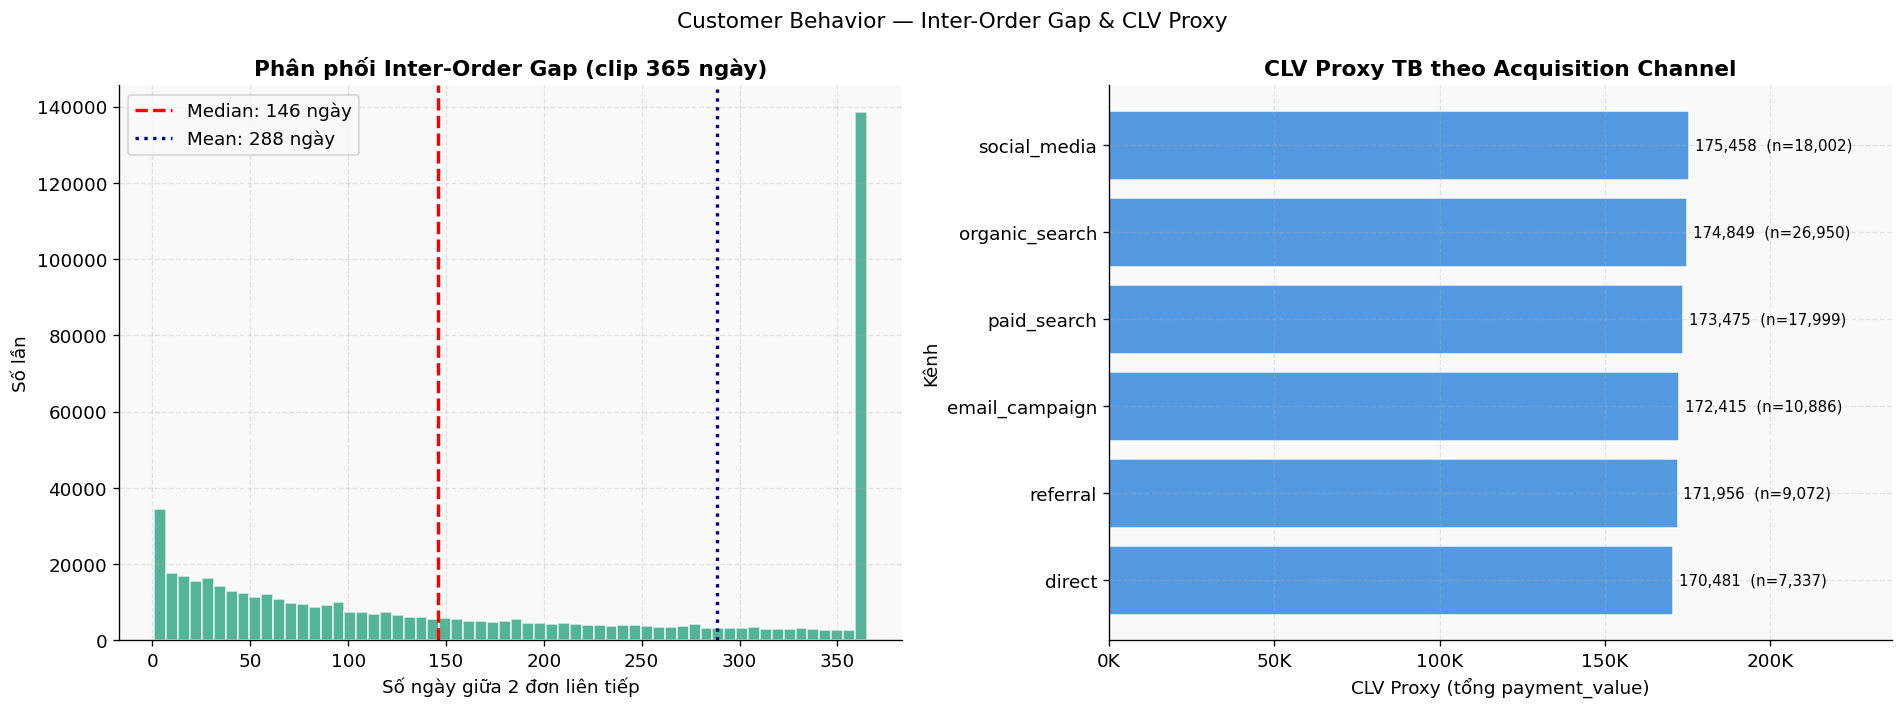
\includegraphics[width=\linewidth]{figures/eda/fig_clv_gap.png}
  \caption{CLV proxy đồng đều kênh (170K–175K); gap trung vị 146 ngày}
  \label{fig:clv}
\end{subfigure}
\caption{Cấu trúc doanh thu theo danh mục và hành vi mua lại.}
\end{figure}

\begin{figure}[htbp]
\centering
\begin{subfigure}[b]{0.49\linewidth}
  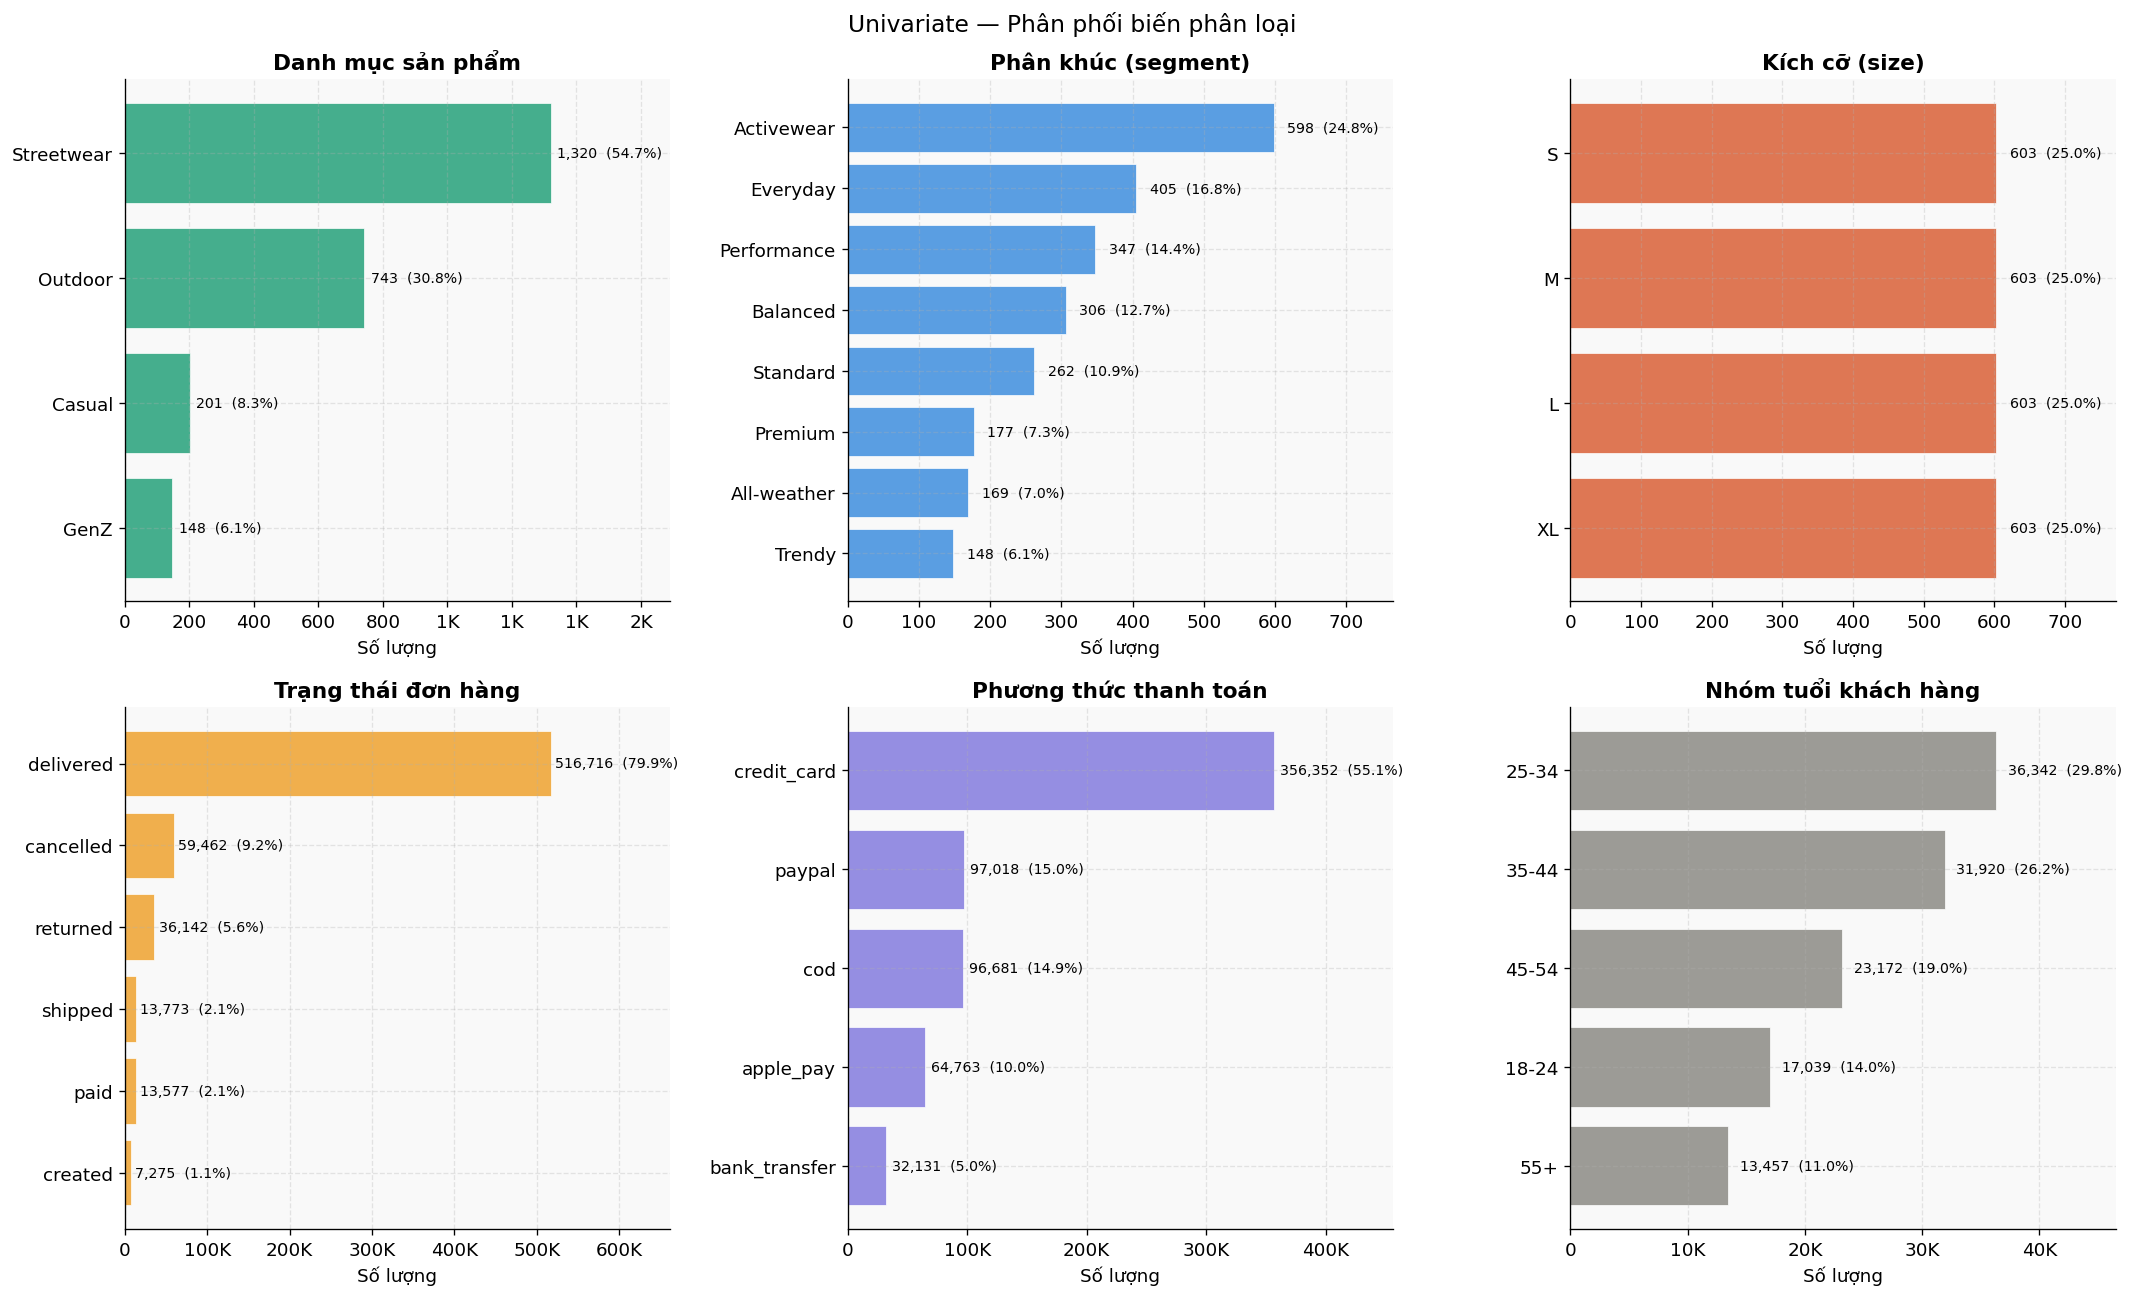
\includegraphics[width=\linewidth]{figures/eda/fig_uni_categorical.png}
  \caption{Phân phối biến phân loại: 79,9\% delivered; credit\_card 55,1\%; 25–34t = 29,8\%}
  \label{fig:uni_cat}
\end{subfigure}
\hfill
\begin{subfigure}[b]{0.49\linewidth}
  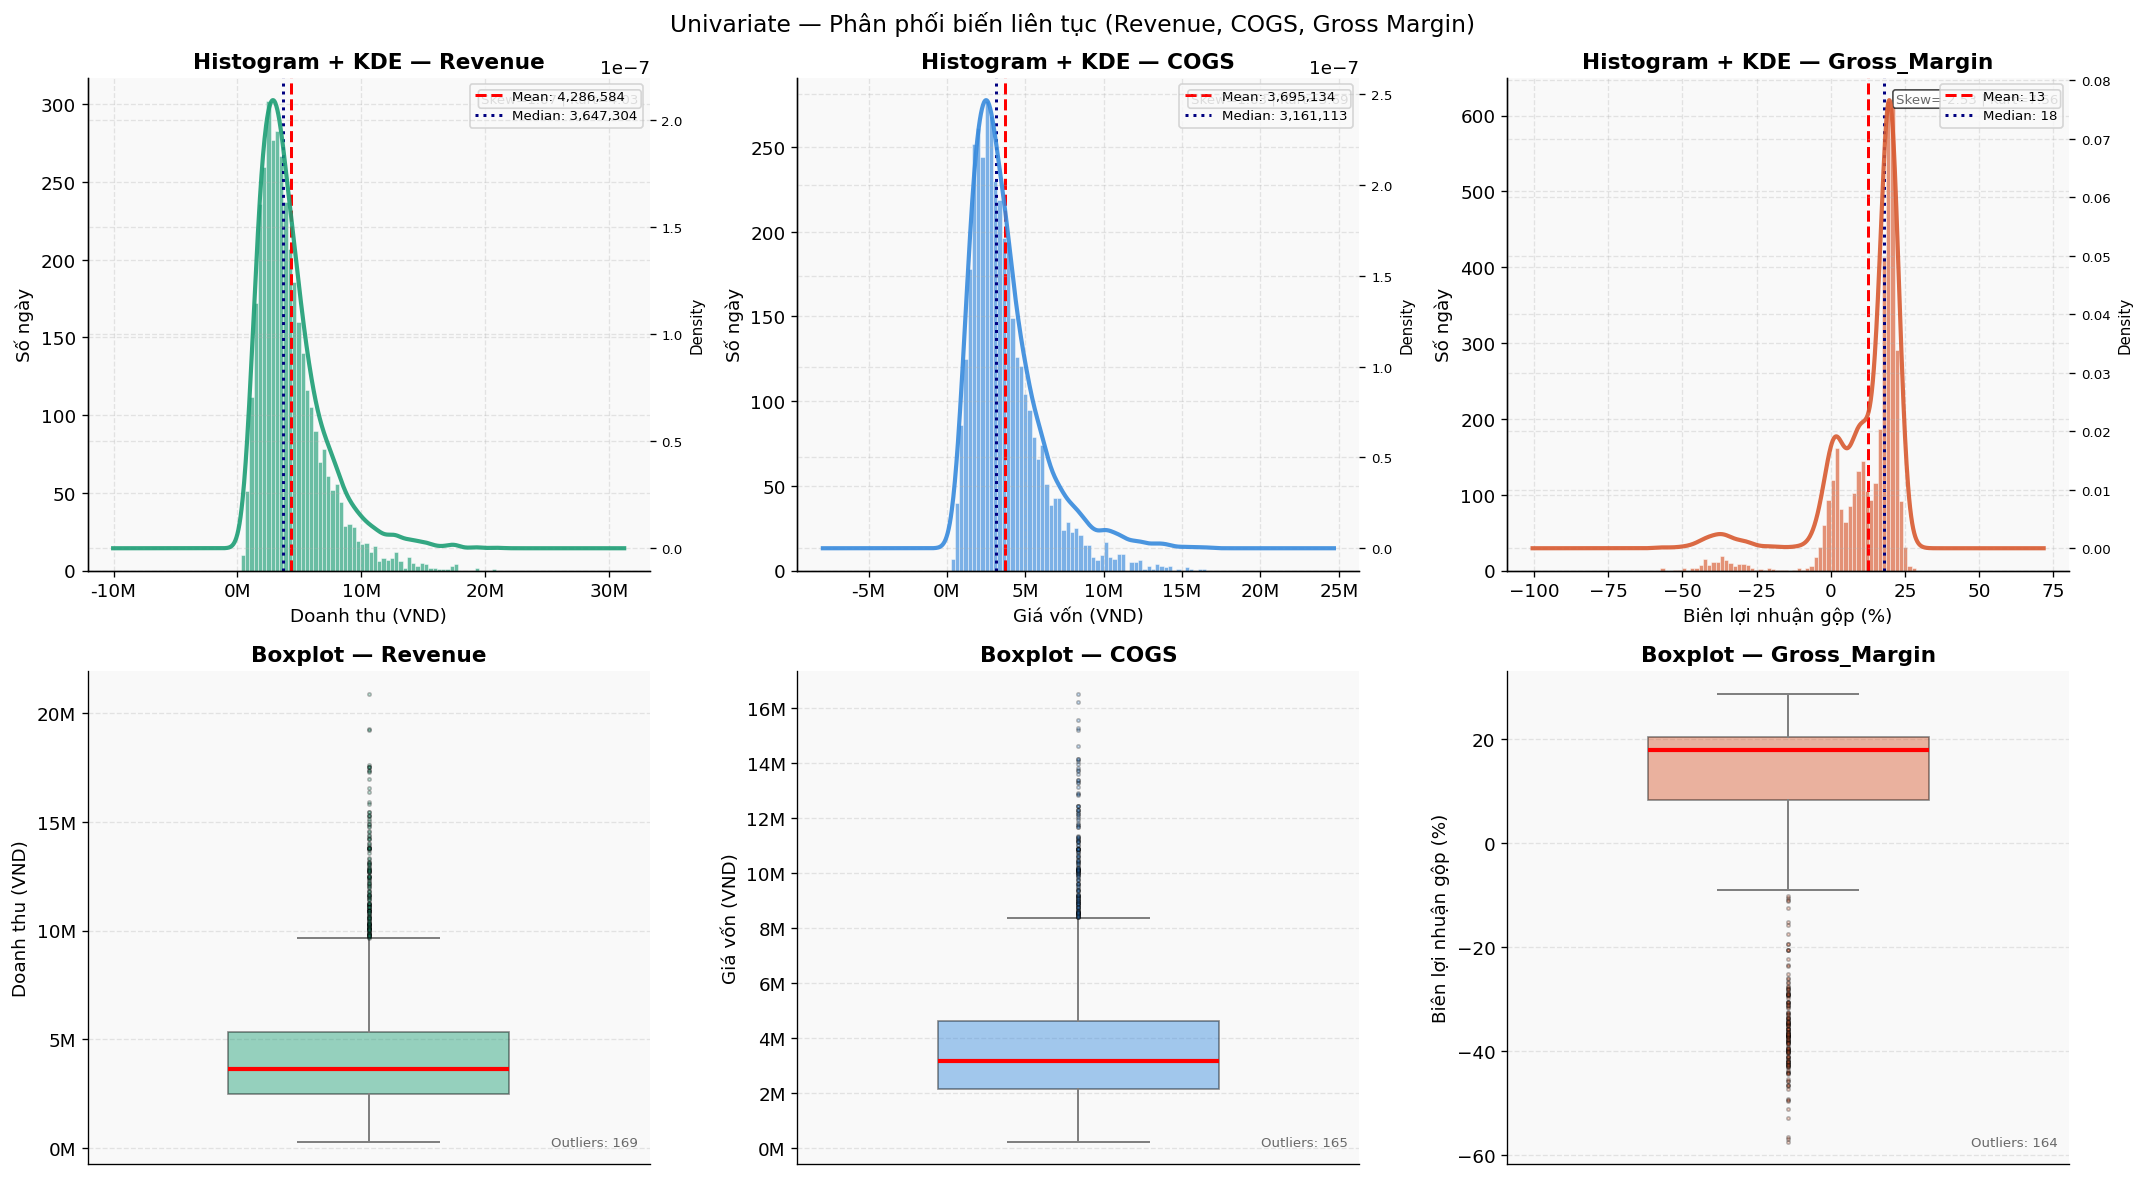
\includegraphics[width=\linewidth]{figures/eda/fig_uni_continuous.png}
  \caption{Revenue, COGS right-skewed (skew$\approx$1,67); Gross Margin bimodal âm}
  \label{fig:uni_cont}
\end{subfigure}
\caption{Phân tích đơn biến.}
\end{figure}

\begin{figure}[htbp]
\centering
\begin{subfigure}[b]{0.49\linewidth}
  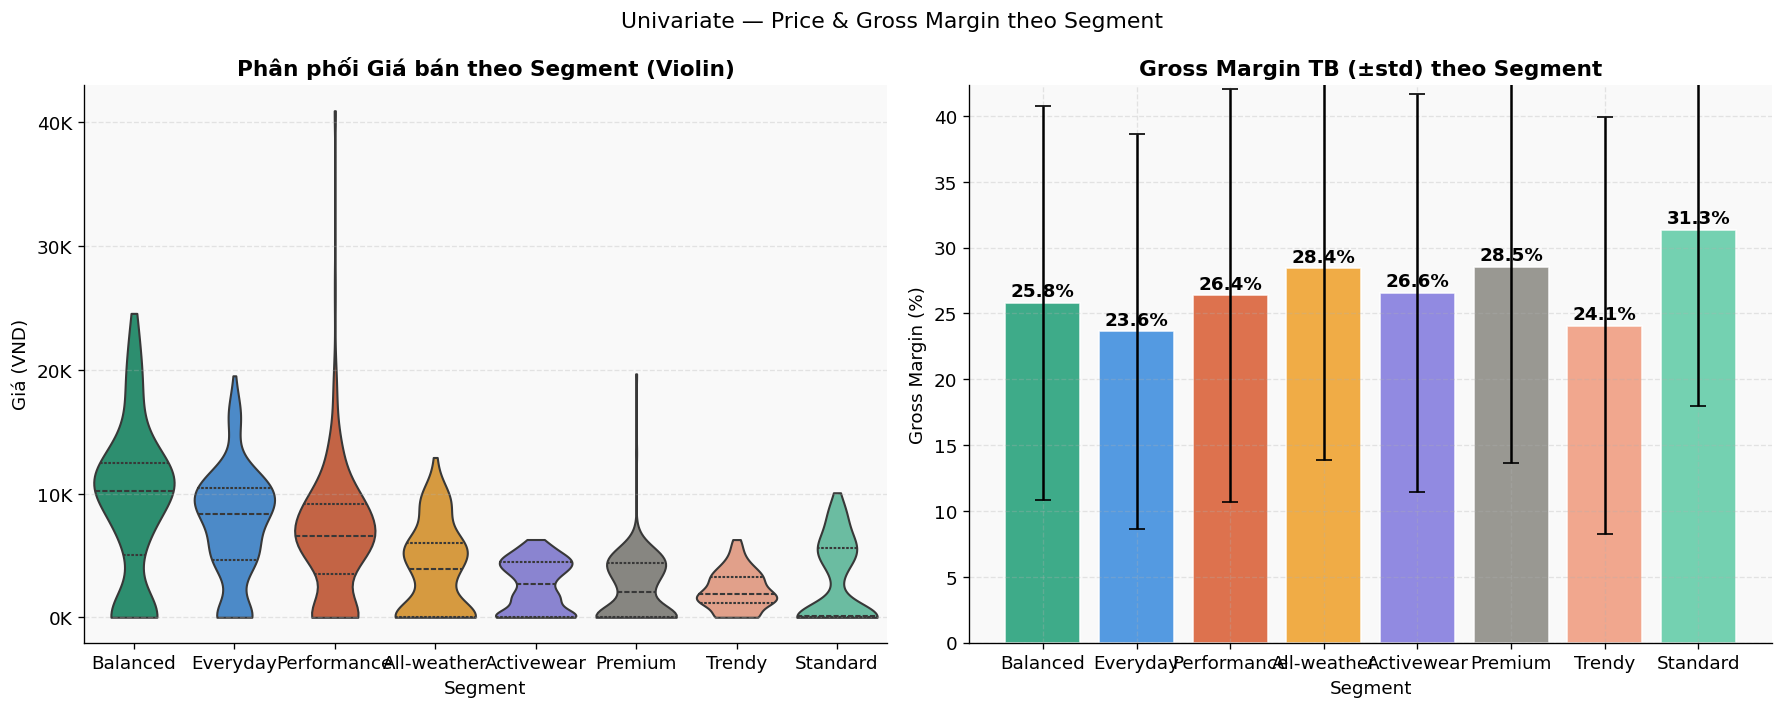
\includegraphics[width=\linewidth]{figures/eda/fig_uni_margin.png}
  \caption{Gross margin theo segment: Standard cao nhất 31,3\%, Everyday thấp nhất 23,6\%}
  \label{fig:uni_margin}
\end{subfigure}
\hfill
\begin{subfigure}[b]{0.49\linewidth}
  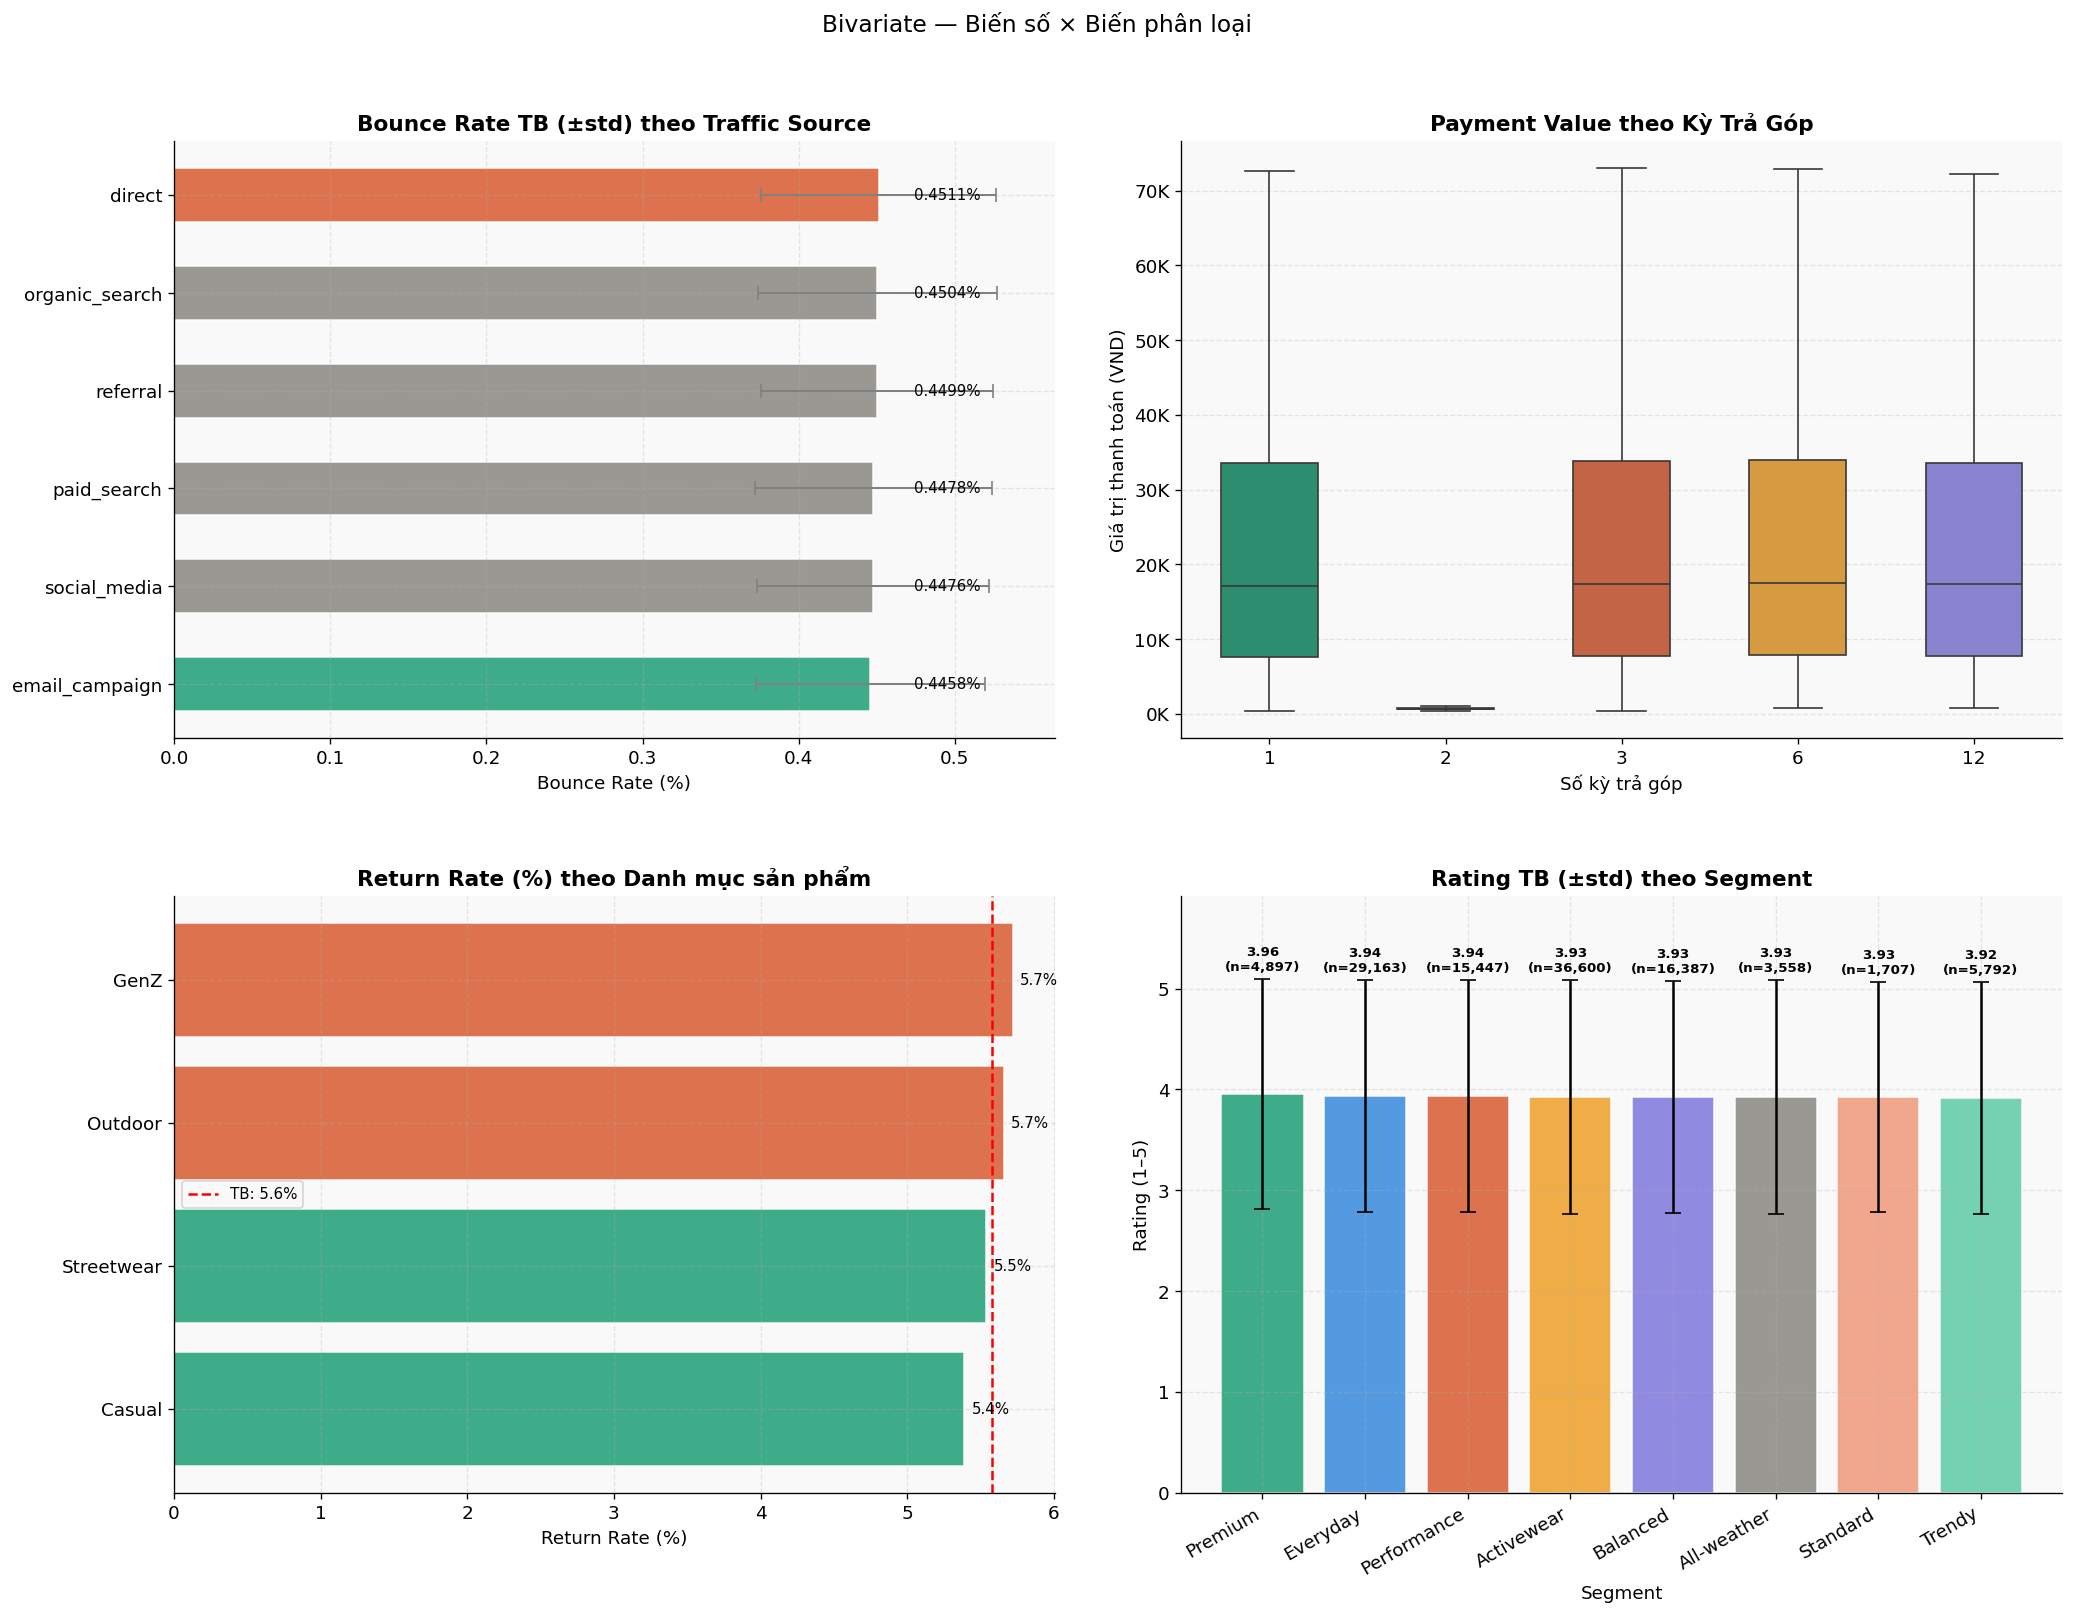
\includegraphics[width=\linewidth]{figures/eda/fig_bi_catnum.png}
  \caption{Bounce rate đồng đều kênh (~44–45\%); return rate cao nhất GenZ + Outdoor (5,7\%)}
  \label{fig:bicat}
\end{subfigure}
\caption{Margin theo phân khúc và phân tích bivariate.}
\end{figure}

\begin{figure}[htbp]
\centering
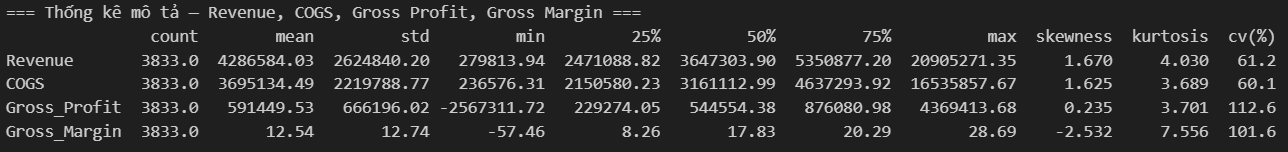
\includegraphics[width=\linewidth]{figures/eda/1.png}
\caption{Thống kê mô tả đầy đủ: Revenue, COGS, Gross Profit, Gross Margin — 3.833 quan sát.}
\label{fig:stats_full}
\end{figure}

% ------------------------------------------------------------------
\clearpage
\section{Chi Tiết Pipeline Mô Hình}
% ------------------------------------------------------------------

\begin{figure}[htbp]
\centering
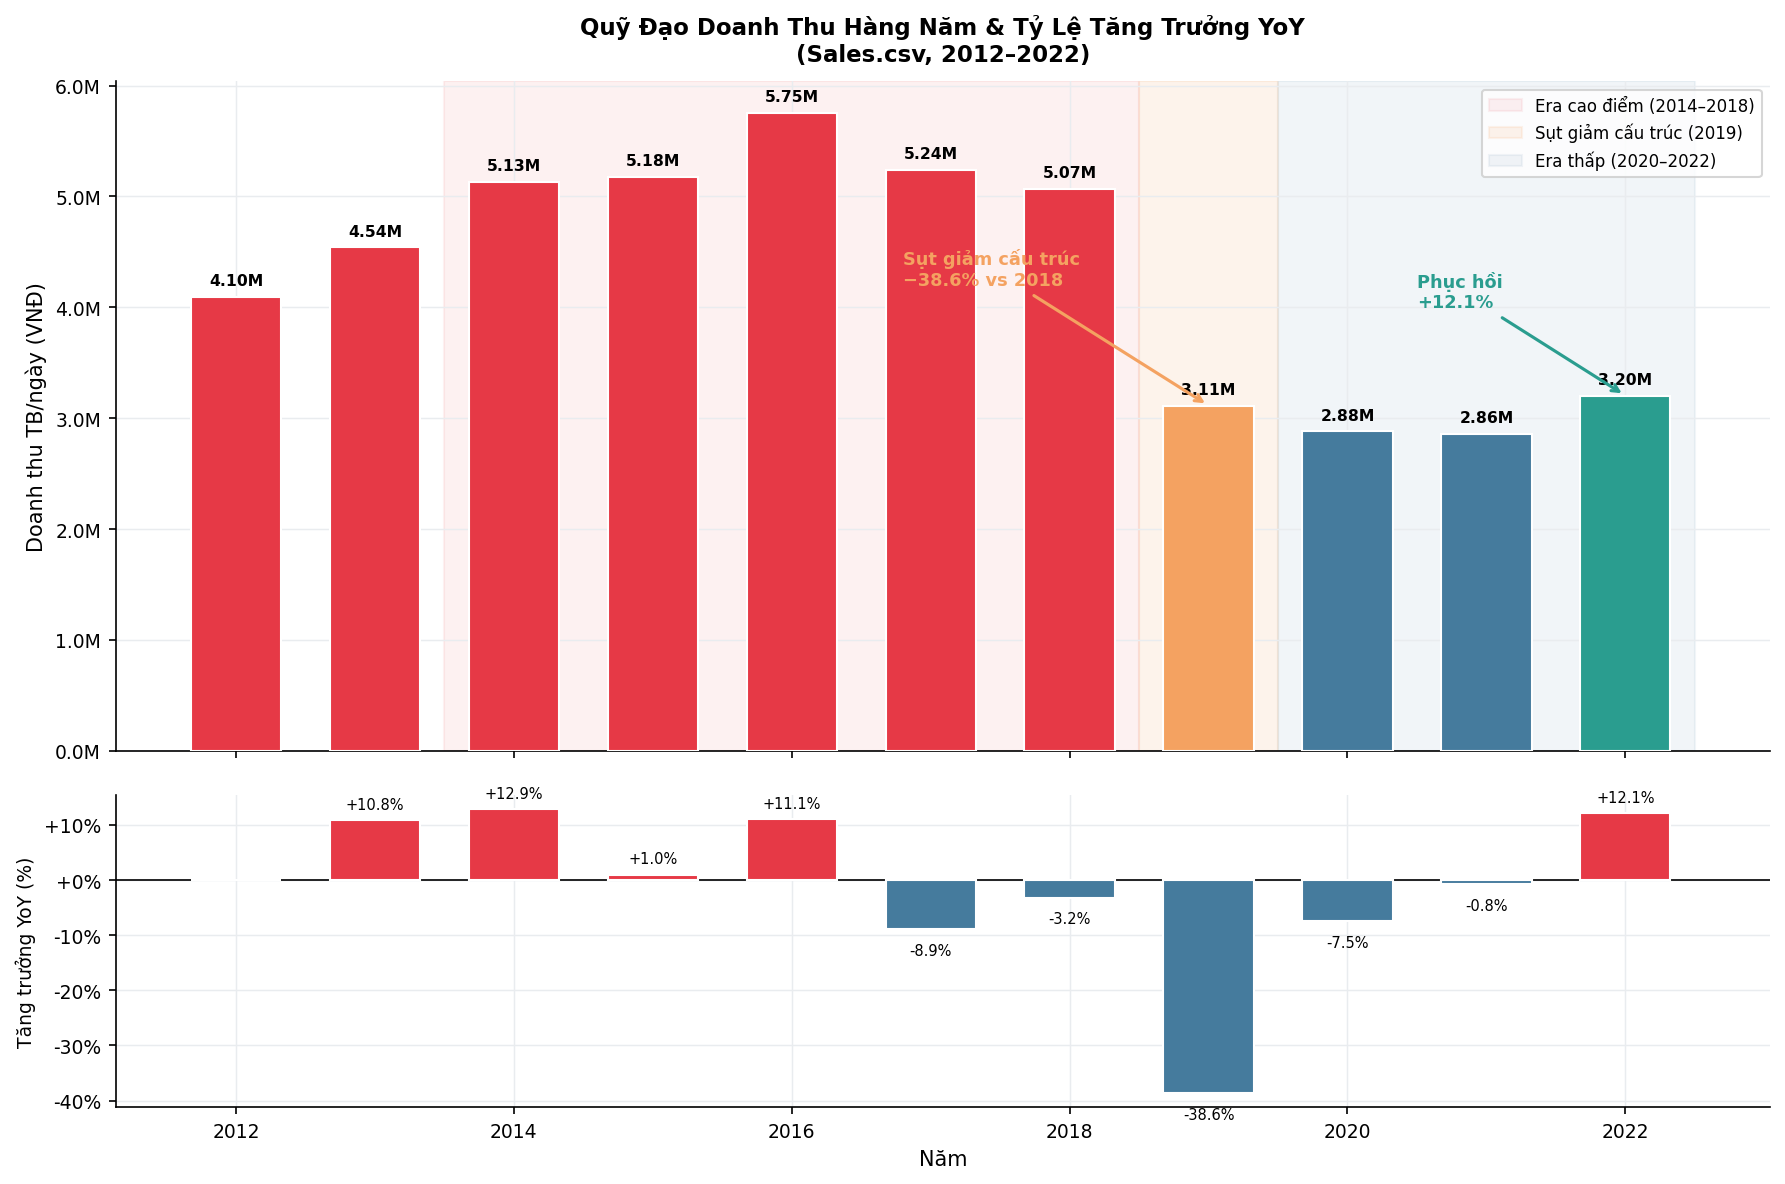
\includegraphics[width=\linewidth]{figures/modelling/fig1_annual_revenue_trajectory.png}
\caption{\textbf{Quỹ đạo doanh thu hàng năm.} Ba era: cao điểm 2014–2018 (~5,27M), sụt $-38,6\%$ năm 2019, phục hồi 2022 (+12,1\%). Cơ sở cho CR calibration.}
\label{fig:annual}
\end{figure}

\begin{figure}[htbp]
\centering
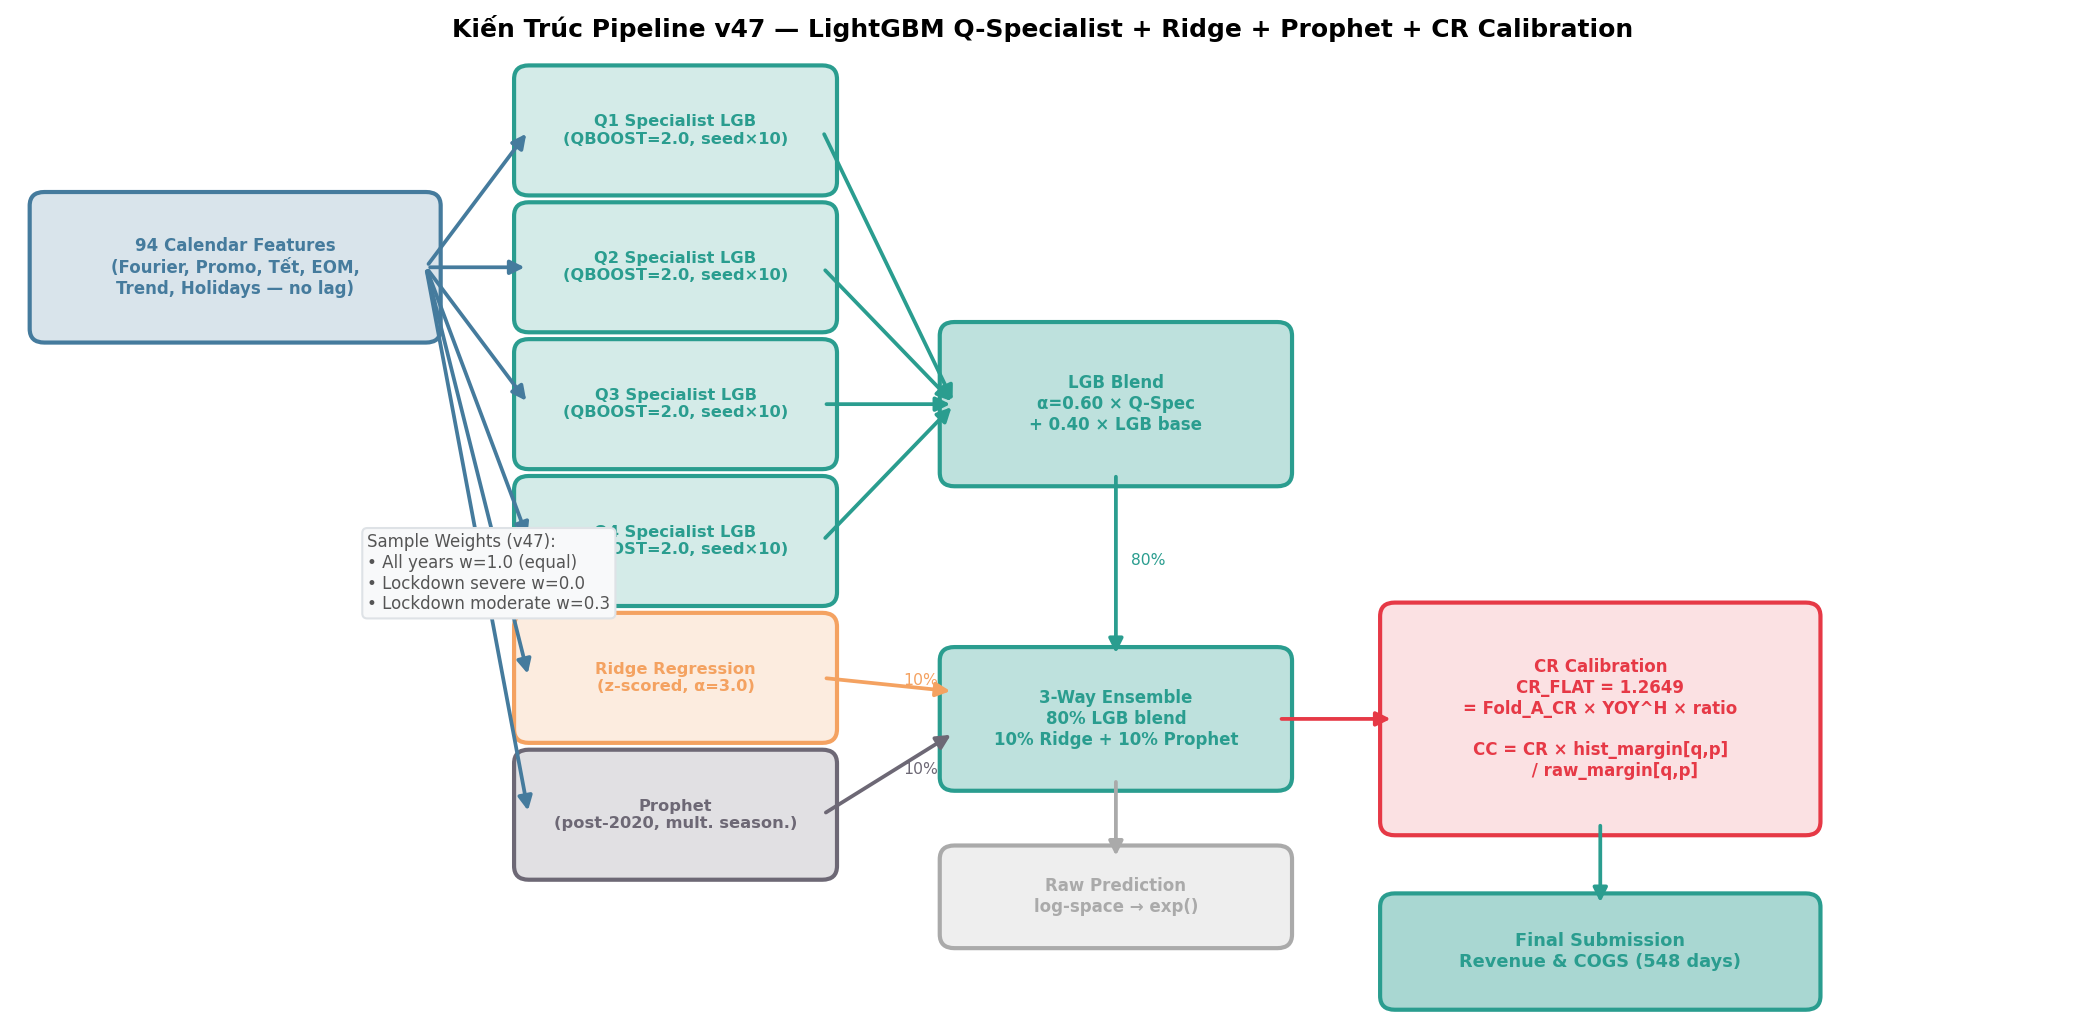
\includegraphics[width=\linewidth]{figures/modelling/fig12_model_architecture.png}
\caption{\textbf{Kiến trúc Pipeline v47.} LGB Q-Specialist (4 quarters × 10 seeds, 80\%) + Ridge (10\%) + Prophet (10\%). CR\_FLAT = 1,2649 là lớp hiệu chỉnh mức độ suy diễn từ dữ liệu huấn luyện.}
\label{fig:architecture}
\end{figure}

\begin{table}[htbp]
\centering
\caption{COGS/Revenue margin theo Quý × Năm Lẻ/Chẵn (dữ liệu $\geq$2020) — cơ sở công thức CC}
\label{tab:margin_qparity}
\small
\begin{tabular}{lcccc}
\toprule
& \textbf{Q1} & \textbf{Q2} & \textbf{Q3} & \textbf{Q4} \\
\midrule
Năm lẻ  & 0,8301 & 0,8306 & \textbf{1,0570} & 0,8917 \\
Năm chẵn & 0,8449 & 0,8404 & 0,8716         & 0,8897 \\
\bottomrule
\end{tabular}
\end{table}

\begin{figure}[htbp]
\centering
\begin{subfigure}[b]{0.49\linewidth}
  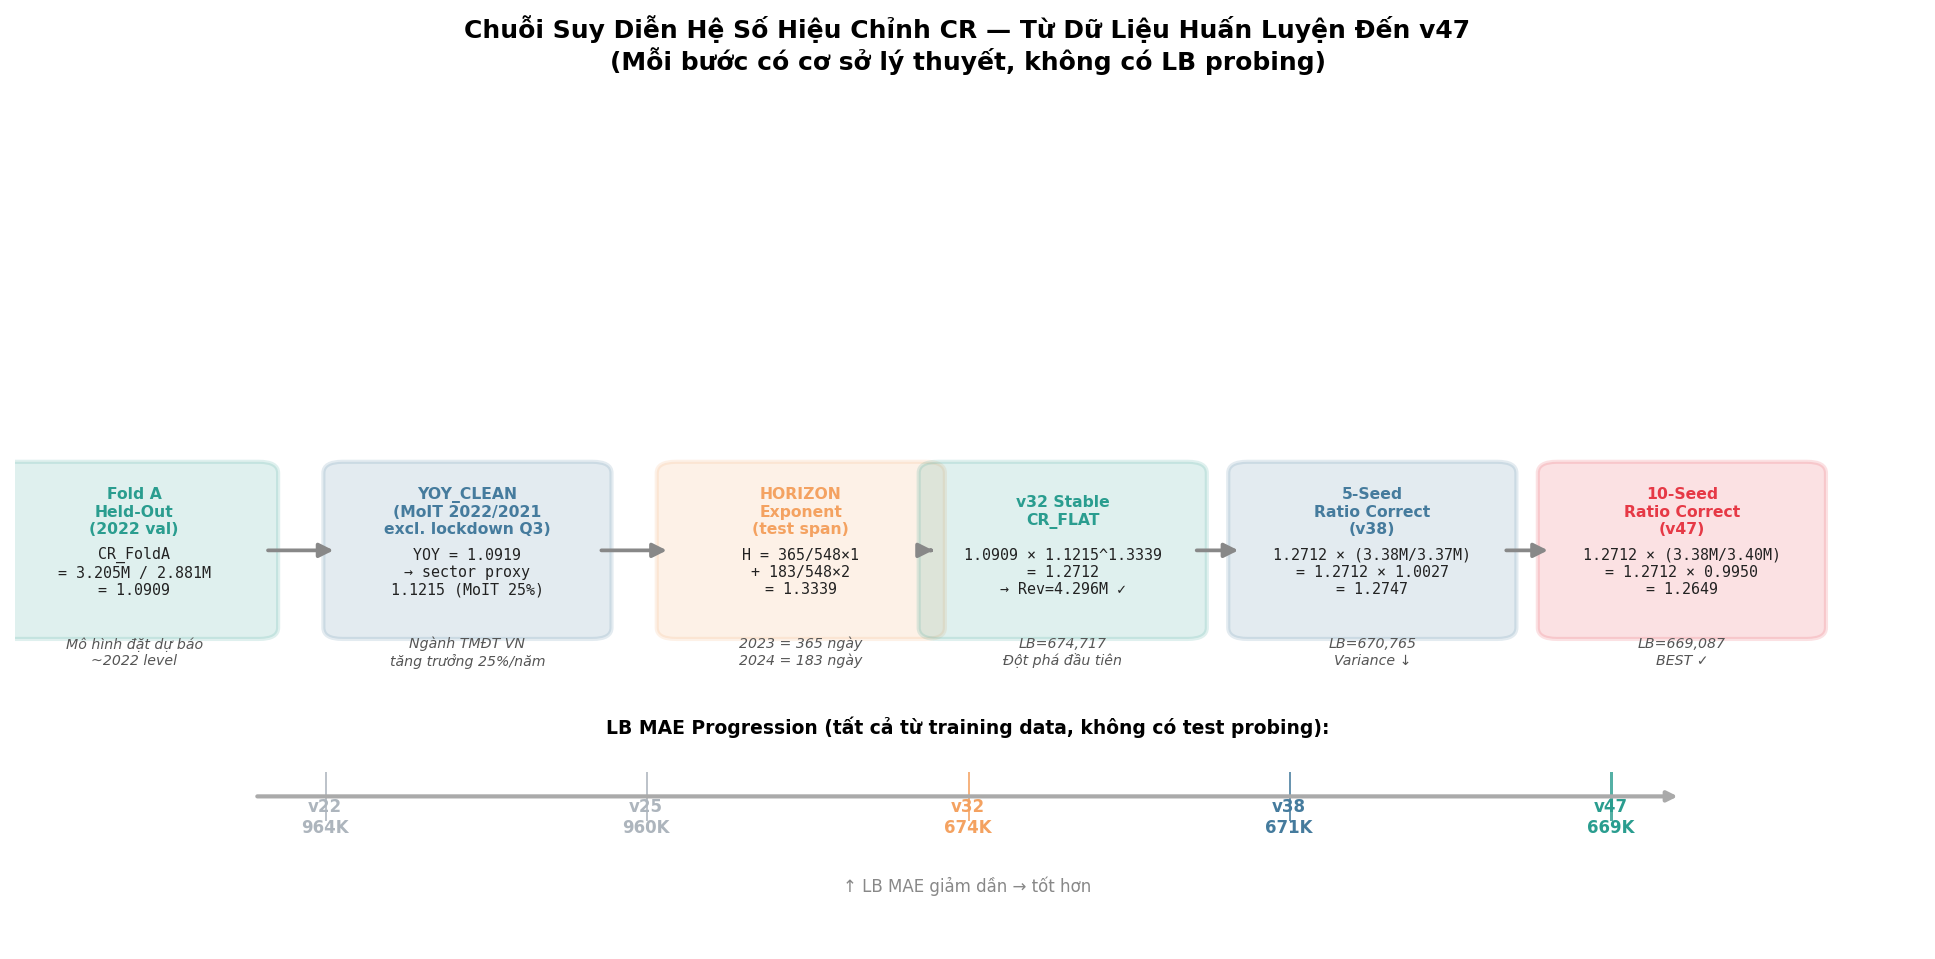
\includegraphics[width=\linewidth]{figures/modelling/fig4_cr_derivation_chain.png}
  \caption{Chuỗi suy diễn CR từ Fold A $\to$ v47 — không có LB probing}
  \label{fig:cr_chain}
\end{subfigure}
\hfill
\begin{subfigure}[b]{0.49\linewidth}
  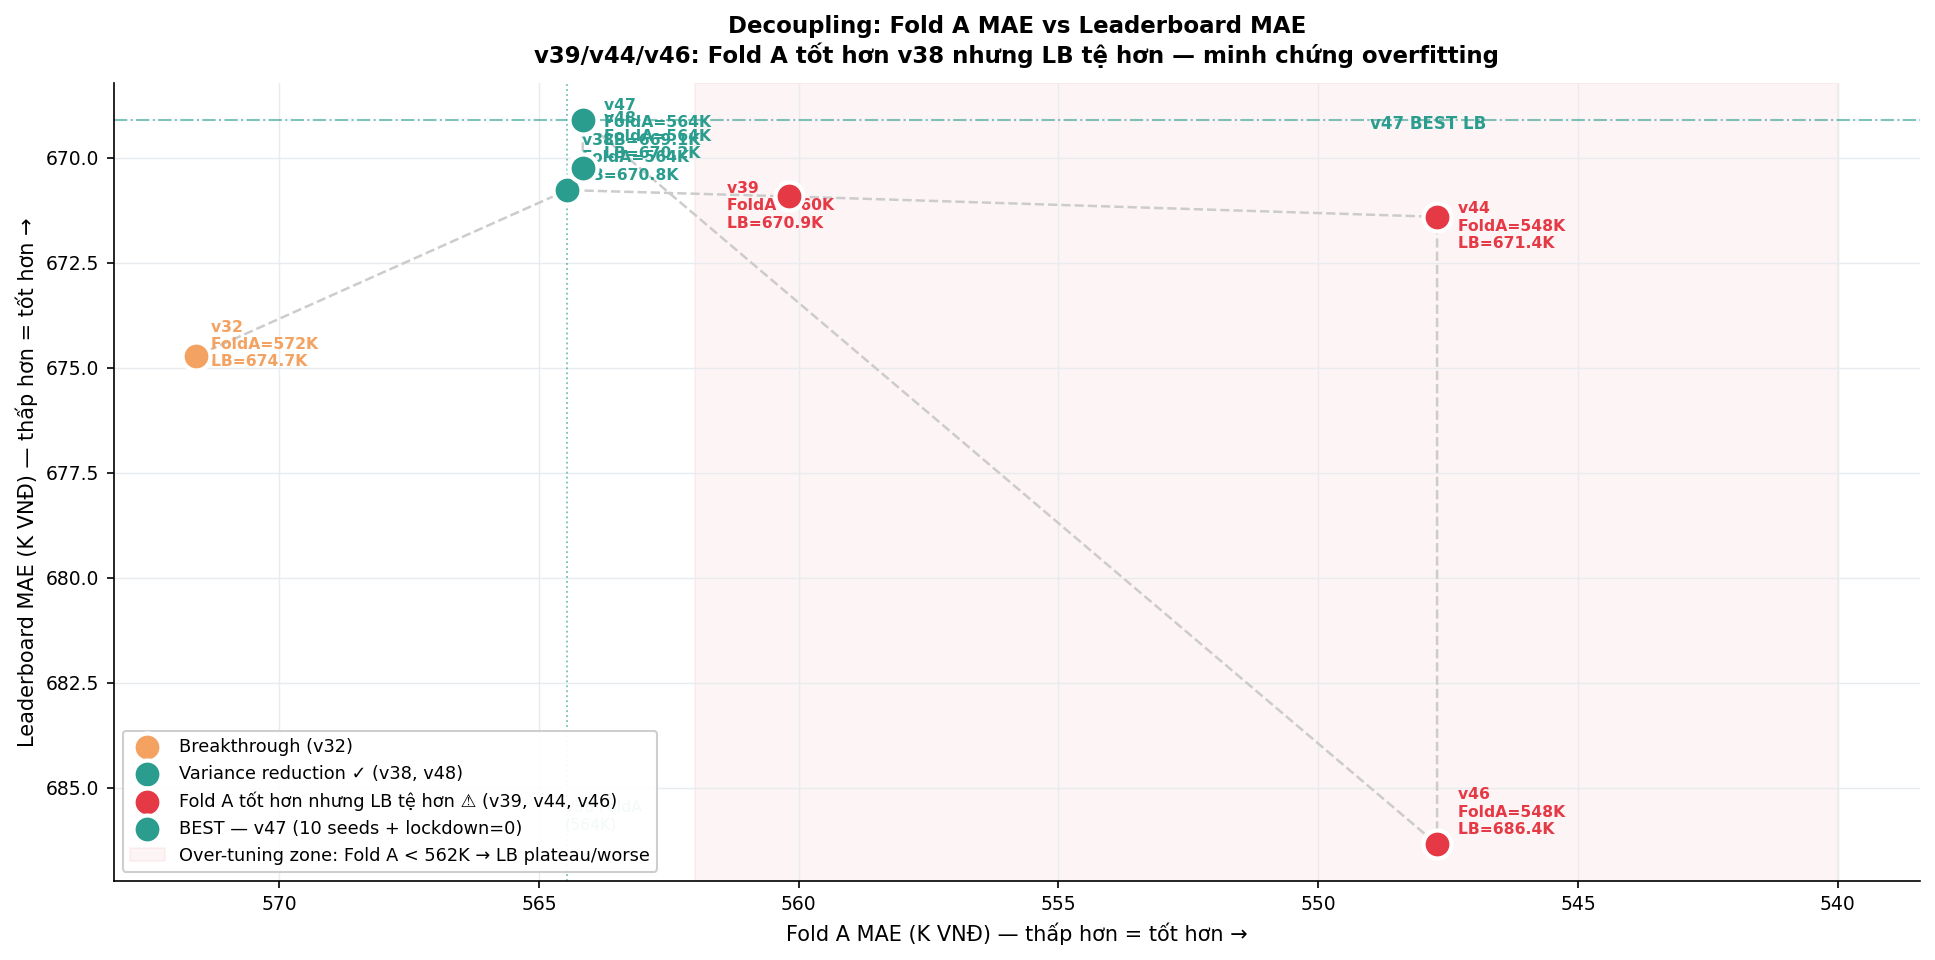
\includegraphics[width=\linewidth]{figures/modelling/fig5_folda_vs_lb_decoupling.png}
  \caption{Decoupling: v39, v44, v46 Fold A tốt hơn nhưng LB tệ hơn}
  \label{fig:decoupling}
\end{subfigure}
\caption{Chuỗi suy diễn CR và hiện tượng decoupling Fold A vs LB.}
\end{figure}

\begin{figure}[htbp]
\centering
\begin{subfigure}[b]{0.49\linewidth}
  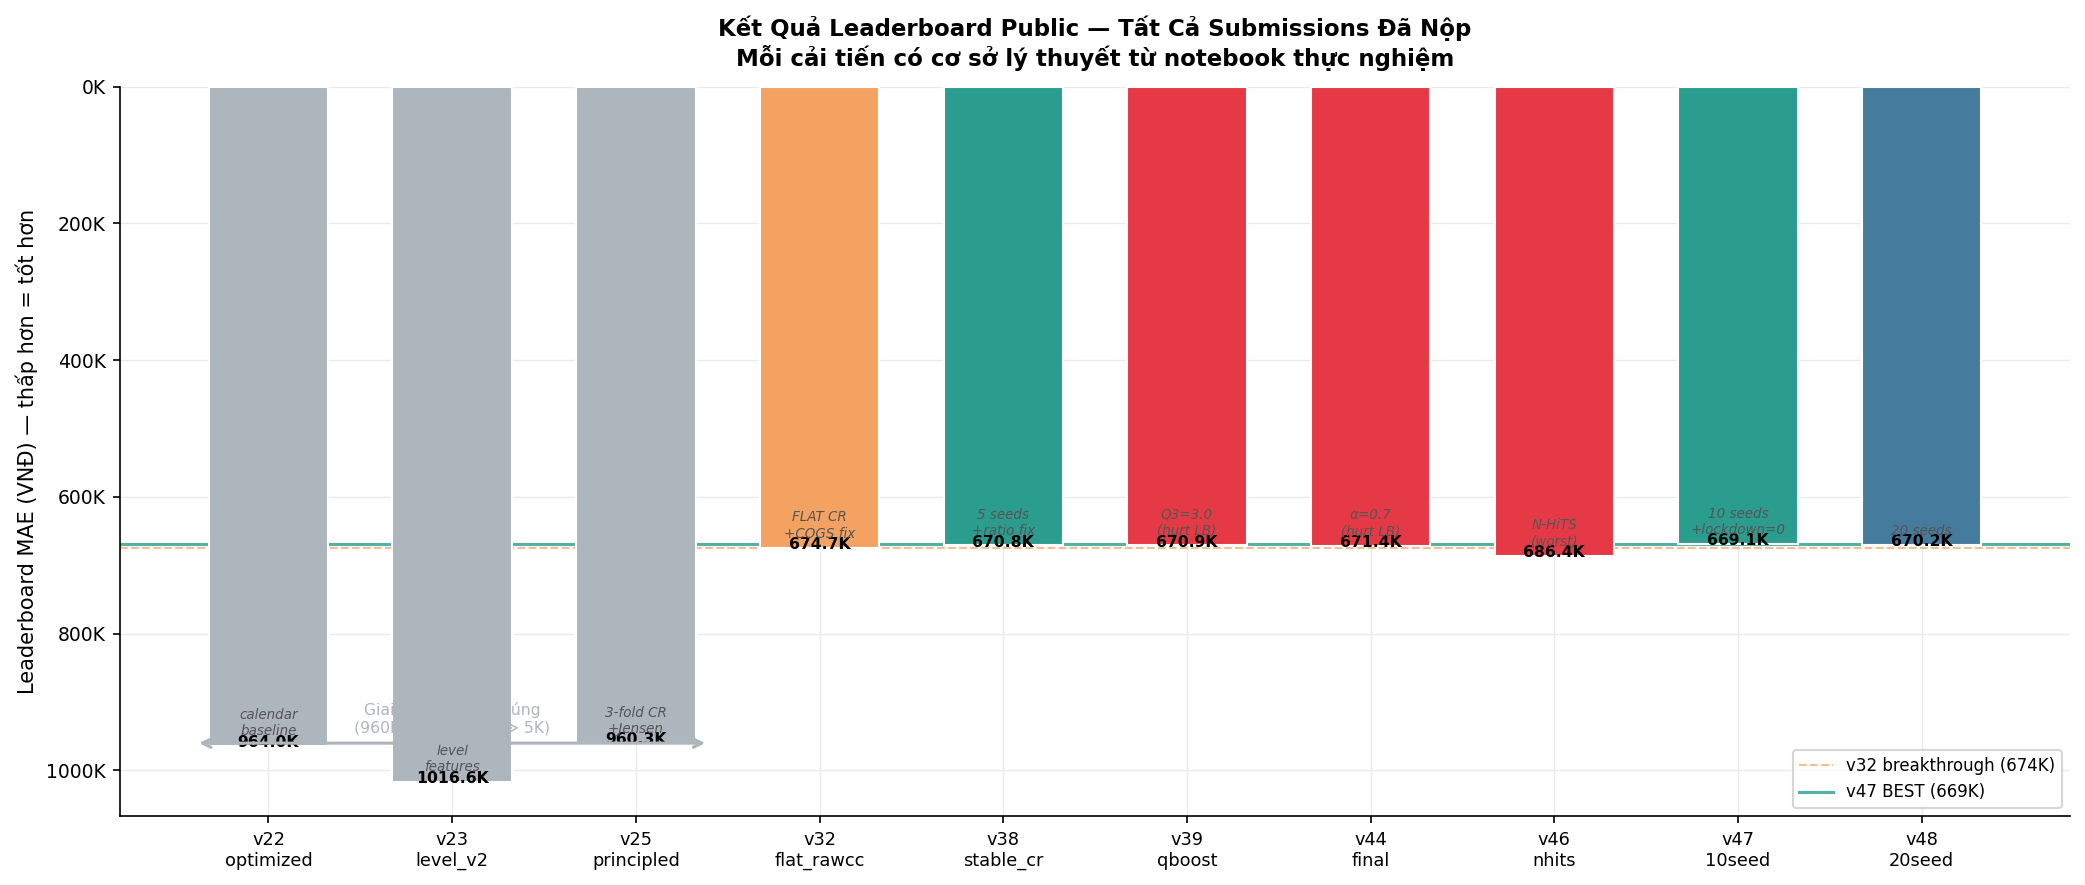
\includegraphics[width=\linewidth]{figures/modelling/fig7_leaderboard_progression.png}
  \caption{Tiến trình LB MAE — đột phá tại v32, cải thiện dần đến v47}
  \label{fig:lb_prog}
\end{subfigure}
\hfill
\begin{subfigure}[b]{0.49\linewidth}
  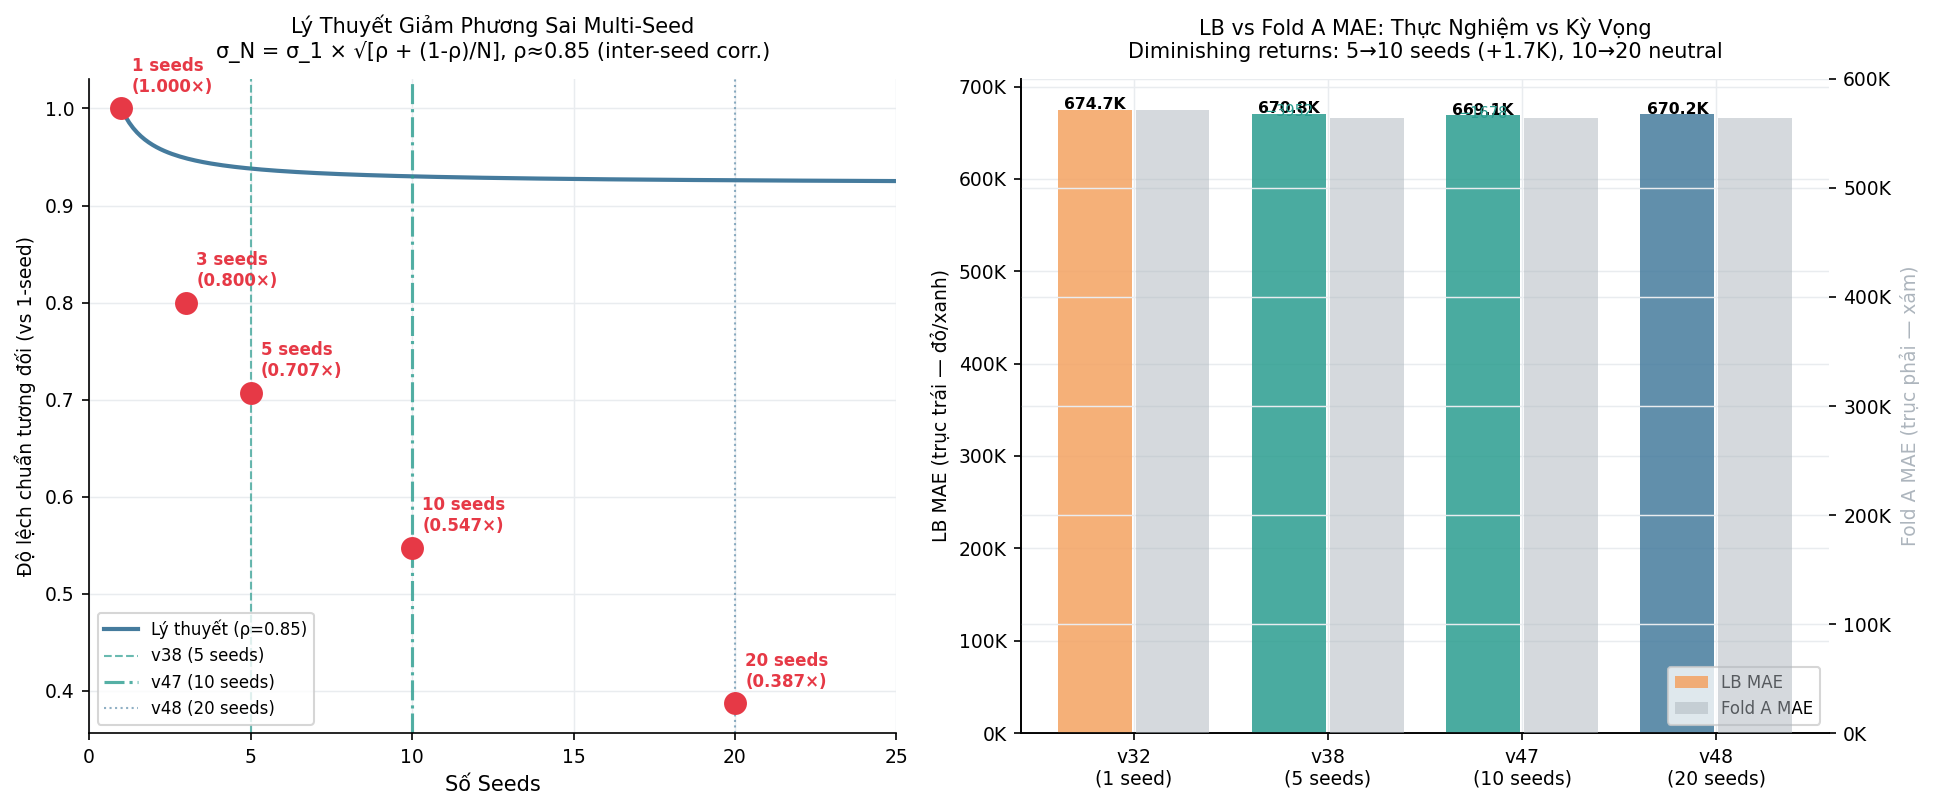
\includegraphics[width=\linewidth]{figures/modelling/fig8_seed_variance_reduction.png}
  \caption{Variance reduction: lý thuyết vs thực nghiệm (5$\to$10 seeds: $-1,7$K LB)}
  \label{fig:seed_var}
\end{subfigure}
\caption{Kết quả LB và hiệu quả giảm phương sai multi-seed.}
\end{figure}

\begin{figure}[htbp]
\centering
\begin{subfigure}[b]{0.49\linewidth}
  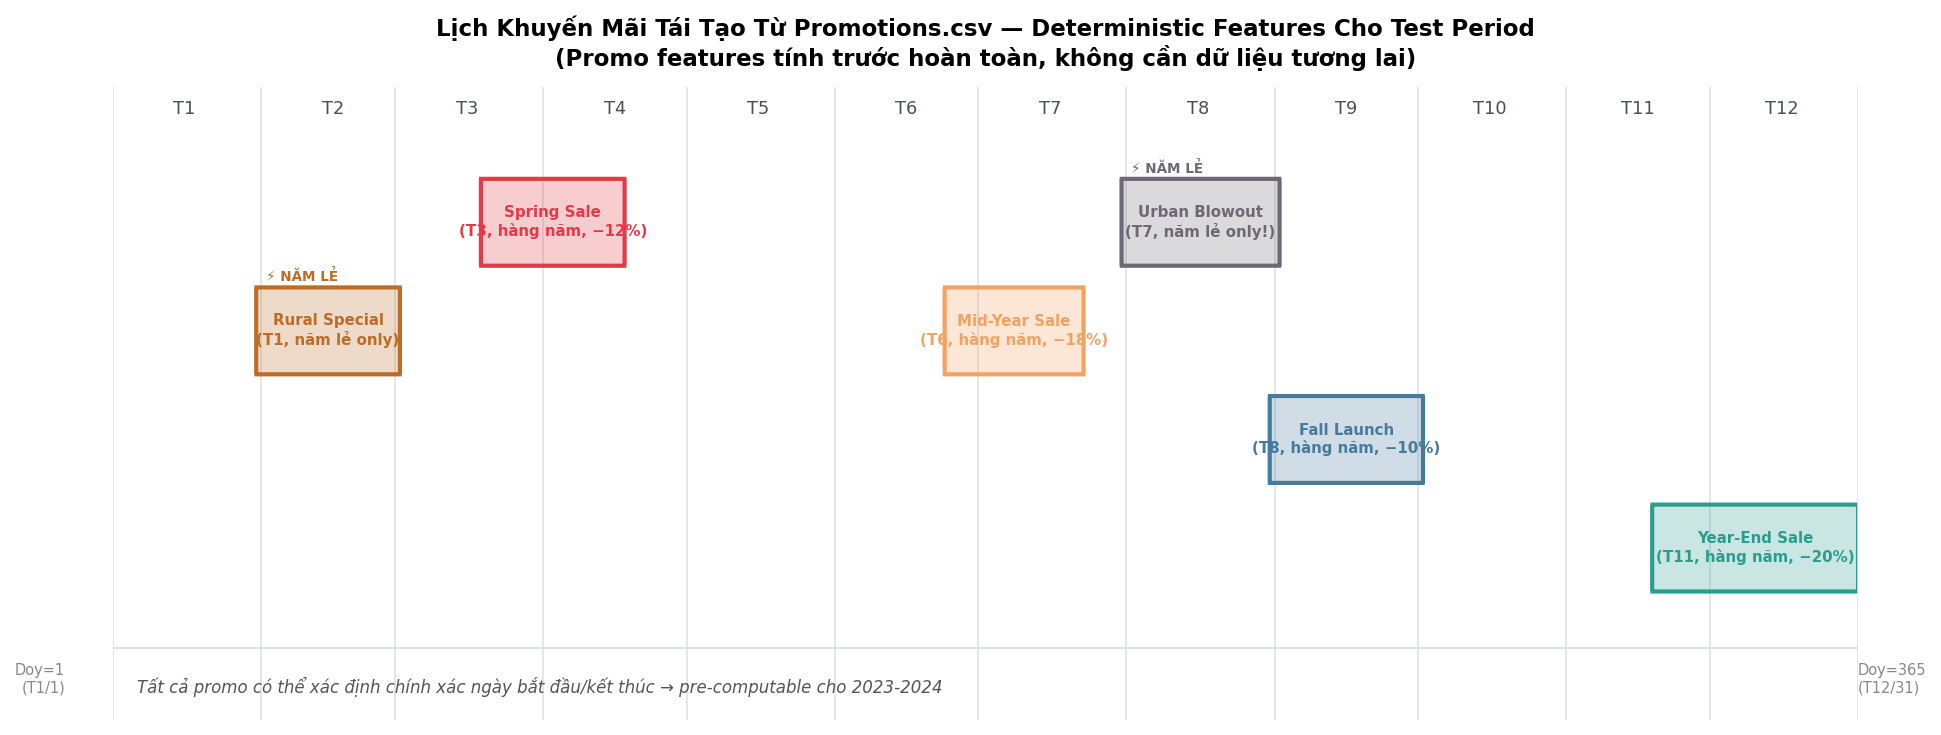
\includegraphics[width=\linewidth]{figures/modelling/fig9_promo_schedule.png}
  \caption{6 chiến dịch tái tạo từ \texttt{promotions.csv} — pre-computable cho 2023–2024}
  \label{fig:promo}
\end{subfigure}
\hfill
\begin{subfigure}[b]{0.49\linewidth}
  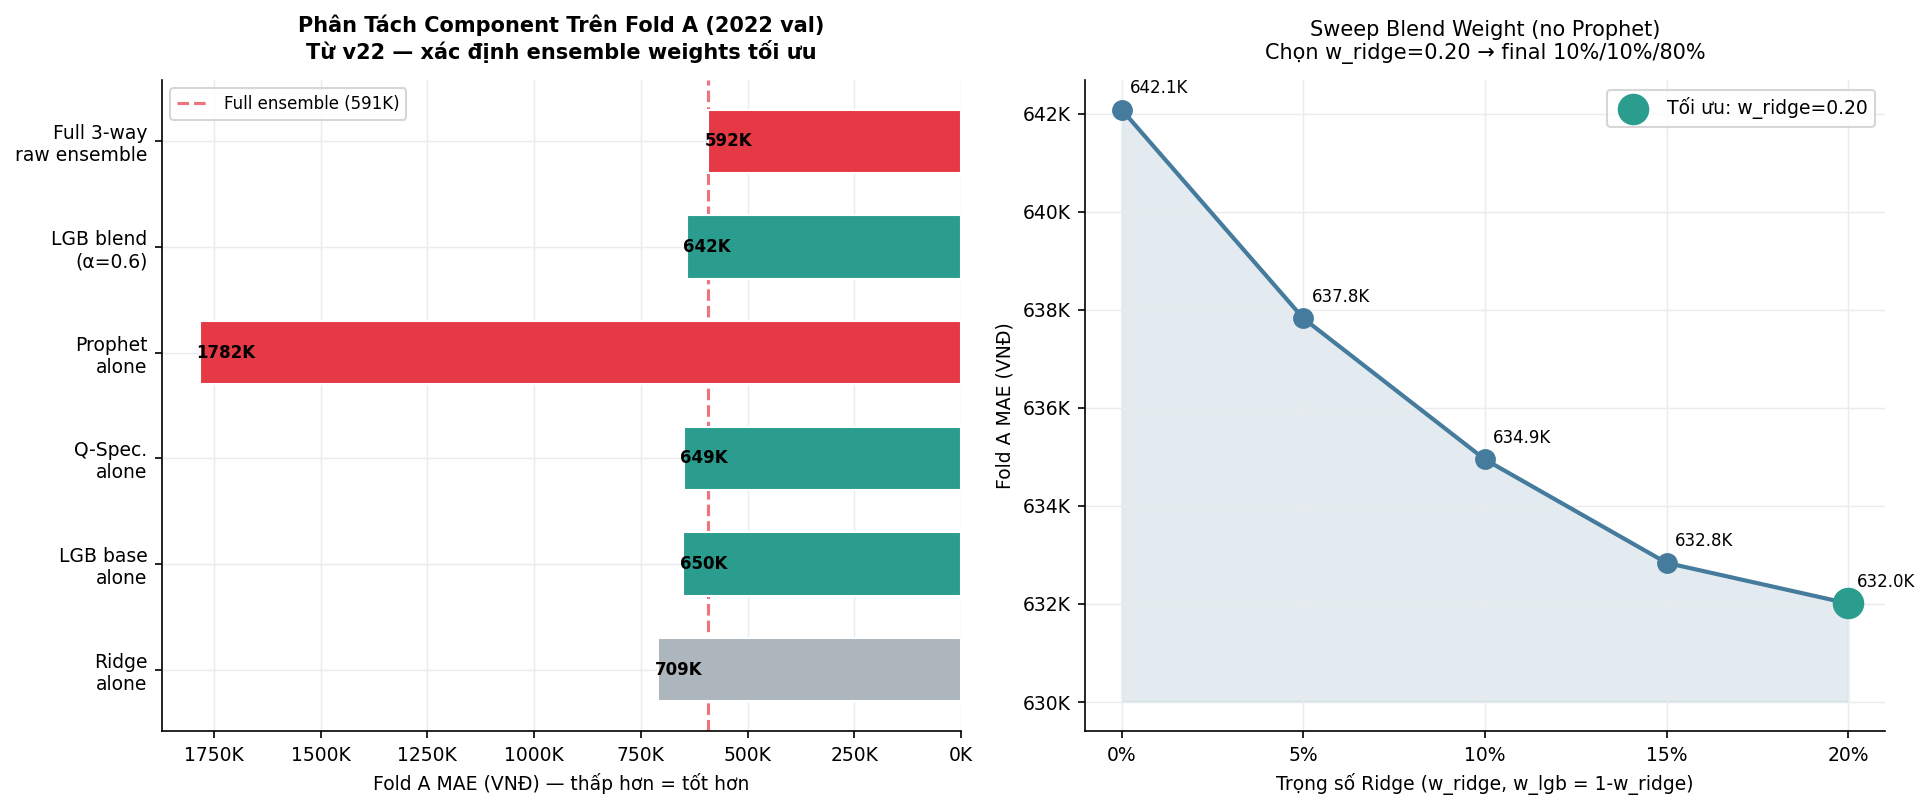
\includegraphics[width=\linewidth]{figures/modelling/fig10_component_analysis.png}
  \caption{Component MAE: Full ensemble (591K) tốt hơn mọi thành phần đơn lẻ}
  \label{fig:component}
\end{subfigure}
\caption{Lịch khuyến mãi deterministic và phân tích component ensemble.}
\end{figure}

\begin{figure}[htbp]
\centering
\begin{subfigure}[b]{0.49\linewidth}
  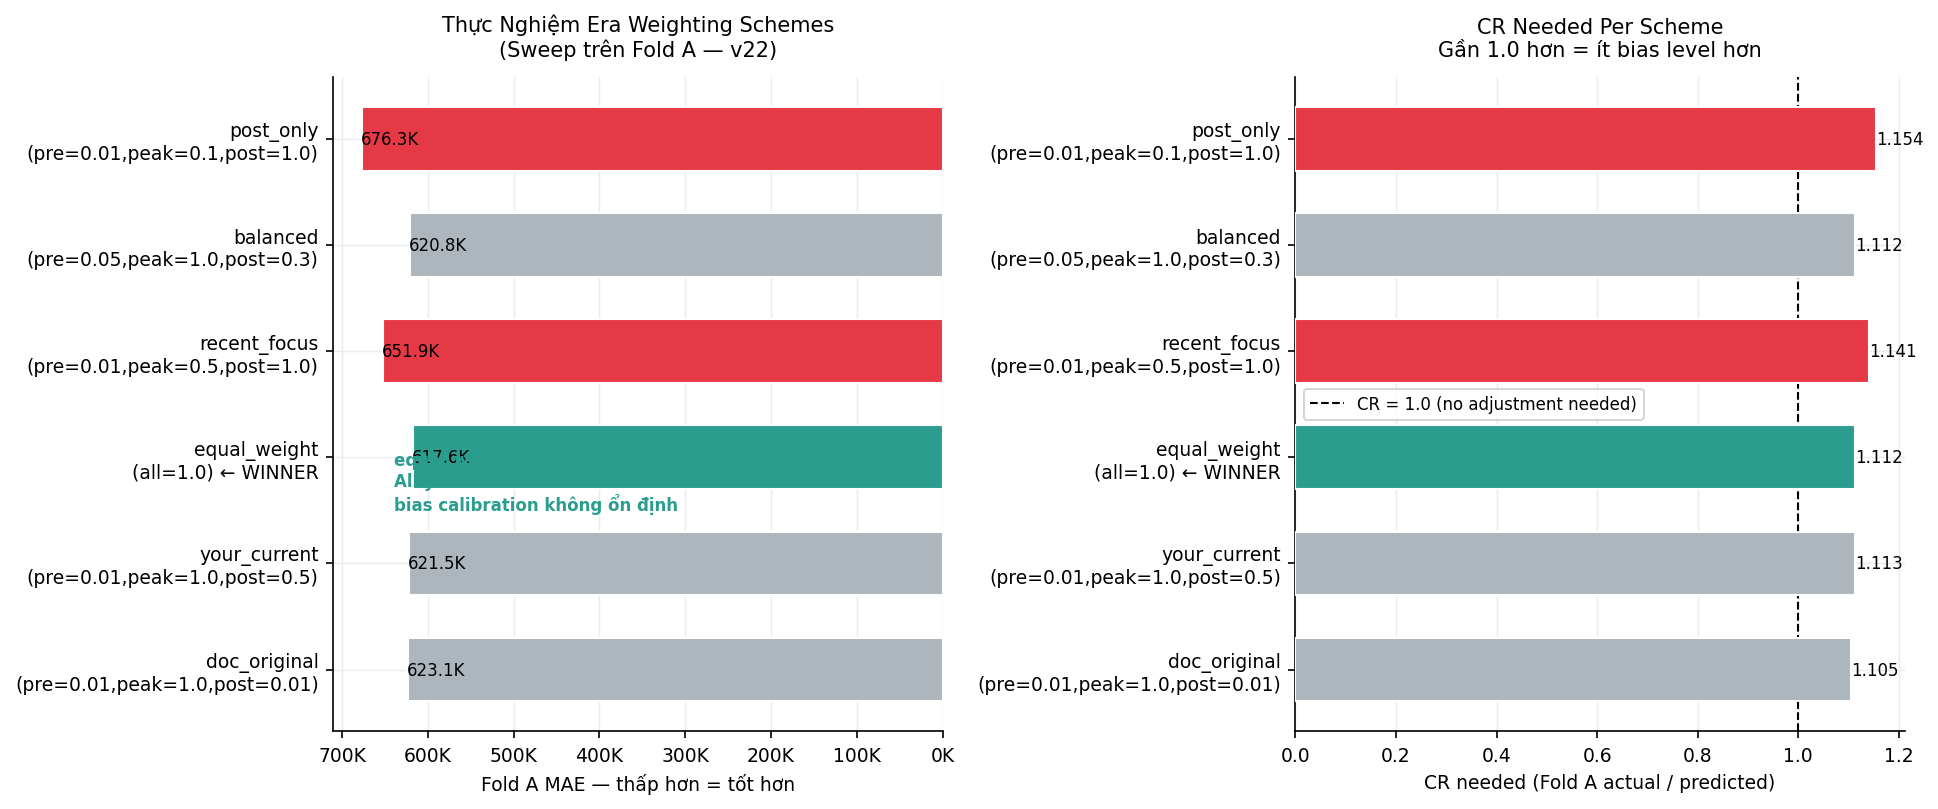
\includegraphics[width=\linewidth]{figures/modelling/fig11_era_weighting_experiment.png}
  \caption{Era weighting sweep: equal-weight tốt nhất Fold A (617K)}
  \label{fig:era_exp}
\end{subfigure}
\hfill
\begin{subfigure}[b]{0.49\linewidth}
  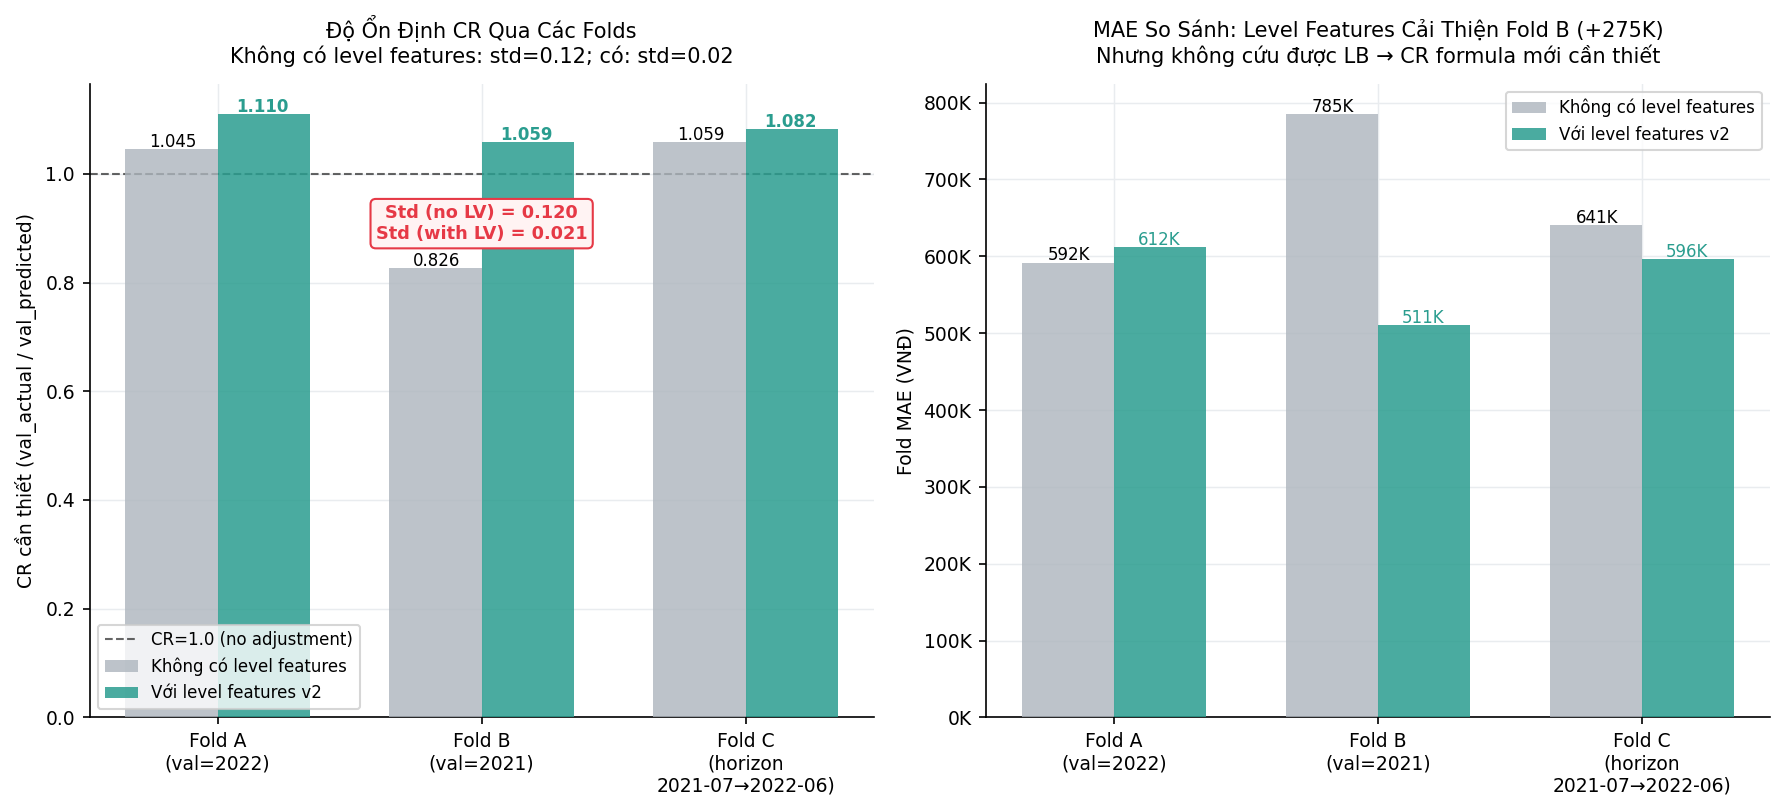
\includegraphics[width=\linewidth]{figures/modelling/fig13_fold_cr_consistency.png}
  \caption{CR consistency: không có level features std=0,12; có level features std=0,02}
  \label{fig:fold_cr}
\end{subfigure}
\caption{Era weighting và ổn định CR cross-fold.}
\end{figure}

\begin{figure}[htbp]
\centering
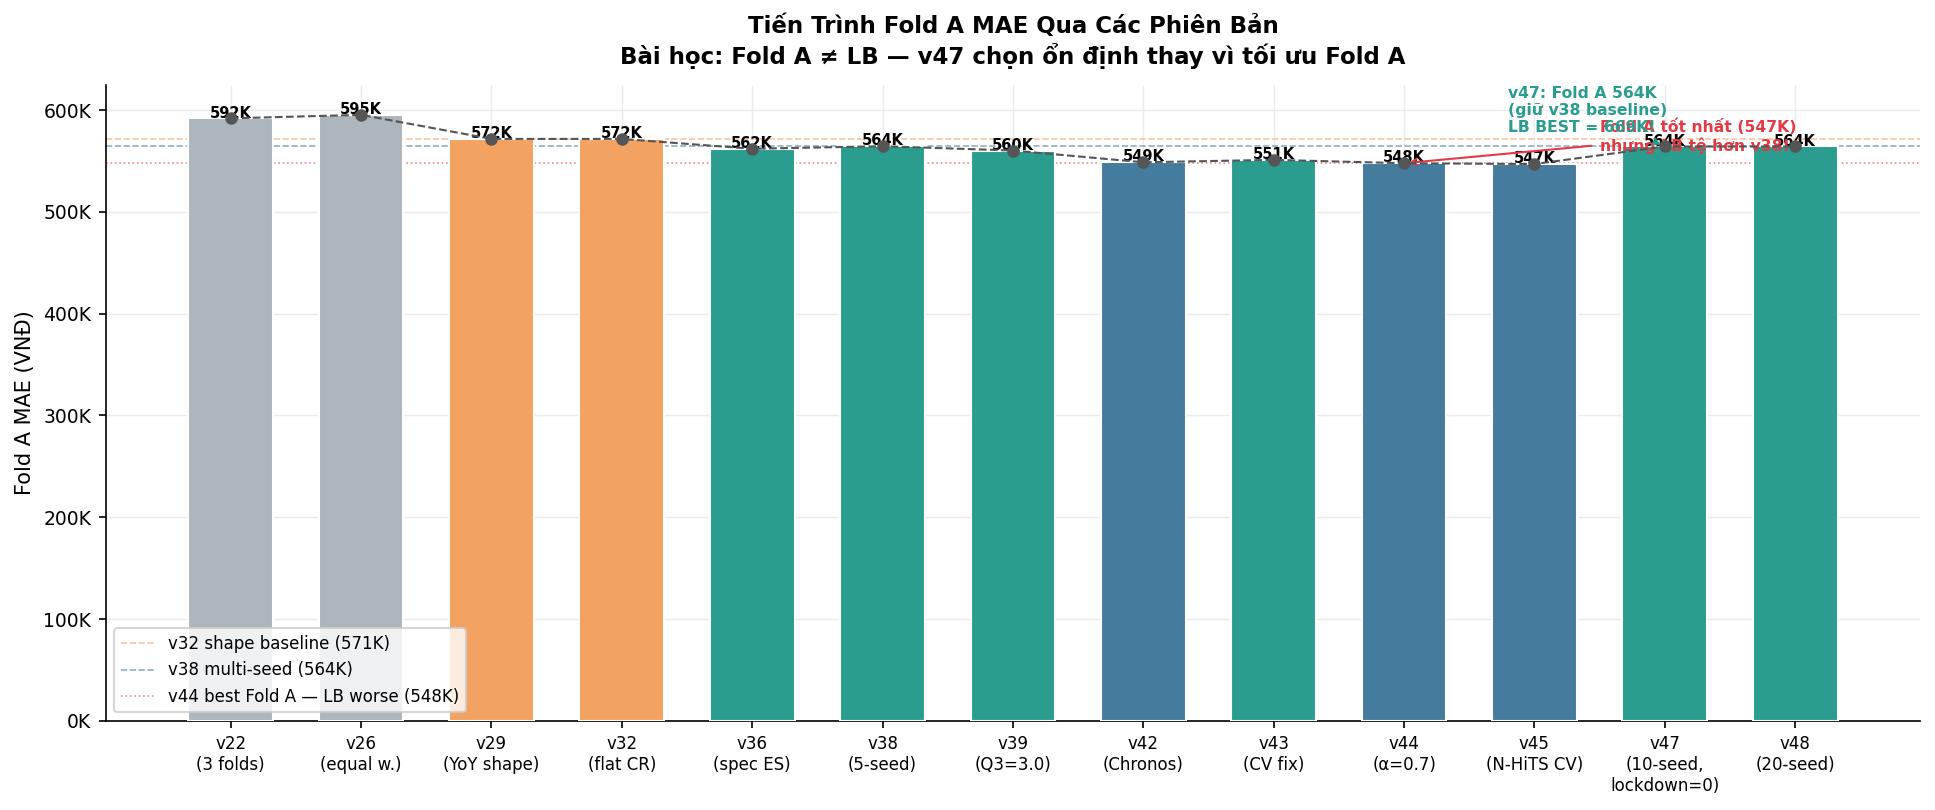
\includegraphics[width=0.82\linewidth]{figures/modelling/fig6_folda_mae_progression.png}
\caption{\textbf{Tiến trình Fold A MAE.} v44 tốt nhất FoldA (548K) nhưng LB tệ nhất. v47 giữ FoldA $\approx$v38, tối ưu bằng multi-seed + lockdown=0.}
\label{fig:folda_prog}
\end{figure}

% ------------------------------------------------------------------
\clearpage
\section{Danh Sách 94 Đặc Trưng \& Hyperparameters}
% ------------------------------------------------------------------

\textbf{Danh sách đầy đủ 94 đặc trưng theo nhóm:}
\begin{itemize}
  \item \textbf{Fourier Năm (10):} sin\_y\{1..5\}, cos\_y\{1..5\}
  \item \textbf{Fourier Tuần (4):} sin\_w\{1,2\}, cos\_w\{1,2\}
  \item \textbf{Fourier Tháng (4):} sin\_m\{1,2\}, cos\_m\{1,2\}
  \item \textbf{Tết (9):} tet\_days\_diff, tet\_intensity, tet\_in\_7/14/30, tet\_before\_7, tet\_after\_7, tet\_on, tet\_post\_recovery
  \item \textbf{Khuyến mãi (24):} promo\_\{spring\_sale, mid\_year, fall\_launch, year\_end, urban\_blowout, rural\_special\}~$\times$~\{flag, since, until, disc\}
  \item \textbf{EOM/Ngày lương (12):} days\_to\_eom, days\_from\_som, dim, is\_eom\_payday, payday\_intensity, is\_last\{1,2,3\}, is\_first\{1,2,3\}
  \item \textbf{Ngày lễ cố định (11):} hol\_\{new\_year, womens\_day, reunification, labor\_day, national\_day, vn\_womens\_day, dd\_1111, dd\_1212, christmas\_eve, christmas, hung\_kings\}
  \item \textbf{Xu hướng \& Chế độ (5):} t\_days, t\_years, regime\_pre2019, regime\_2019, regime\_post2019
  \item \textbf{Lịch cơ bản (15):} year, month, day, dow, doy, quarter, is\_weekend, is\_odd\_year, is\_q1/q2/q3/q4, q3\_odd\_year, hol\_black\_friday
\end{itemize}

\textbf{Hyperparameters LGB (v47):} objective=regression, metric=mae, learning\_rate=0,03, num\_leaves=63, min\_data\_in\_leaf=30, feature\_fraction=0,85, bagging\_fraction=0,85, bagging\_freq=5, lambda\_l2=1,0.

\textbf{Seeds (10):} [42, 137, 314, 271, 999, 1234, 2718, 3141, 7777, 9999].

\textbf{Môi trường:} Kaggle Notebook, Python 3.10. Tất cả seeds cố định. Không dùng dữ liệu ngoài bộ được cung cấp (ngoài báo cáo MoIT 2022 public).

% ------------------------------------------------------------------
\clearpage
\section{SHAP Phân Tích Chi Tiết}
% ------------------------------------------------------------------

\begin{figure}[htbp]
\centering
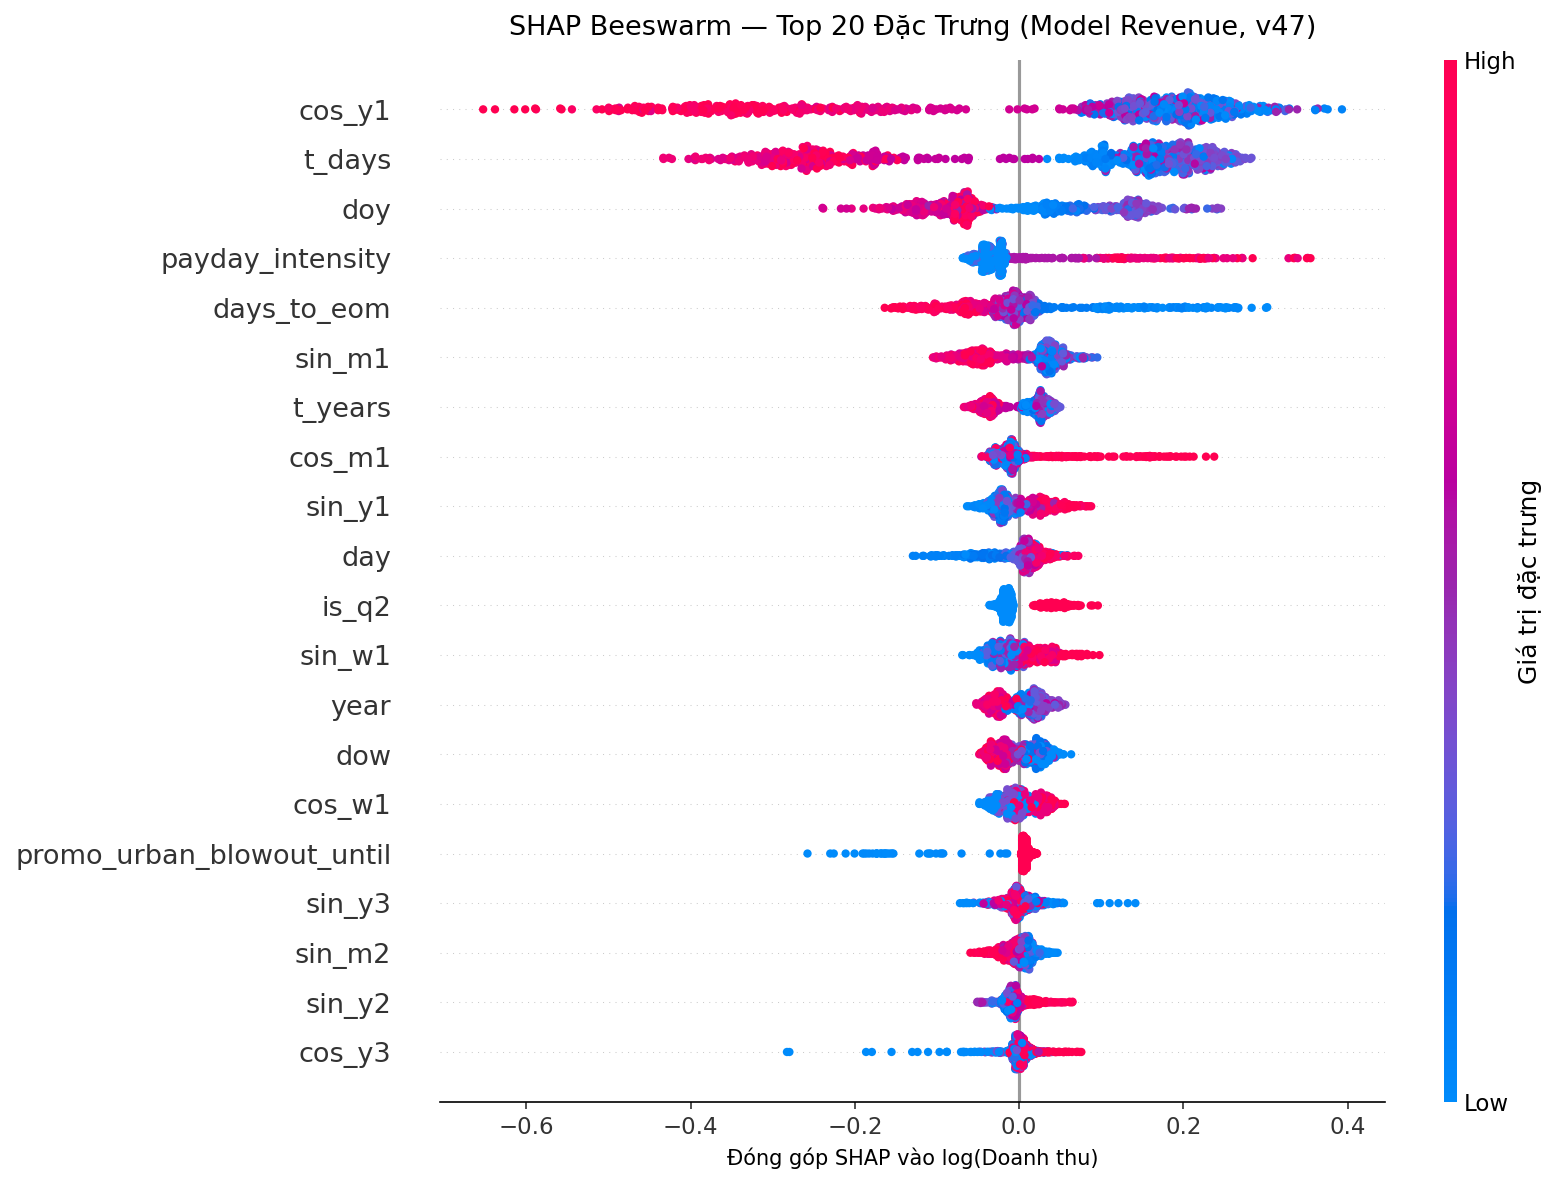
\includegraphics[width=\linewidth]{figures/shap/shap_summary_beeswarm.png}
\caption{\textbf{SHAP Beeswarm — Top 20 features.} cos\_y1: đỏ (T4–T6) $\to$ SHAP $+0,3$; xanh (T11–T12) $\to$ SHAP $-0,6$. t\_days: xanh đậm (2014–2018) $\to$ $+0,4$; đỏ (2020–2022) $\to$ $-0,5$.}
\label{fig:beeswarm}
\end{figure}

\begin{figure}[htbp]
\centering
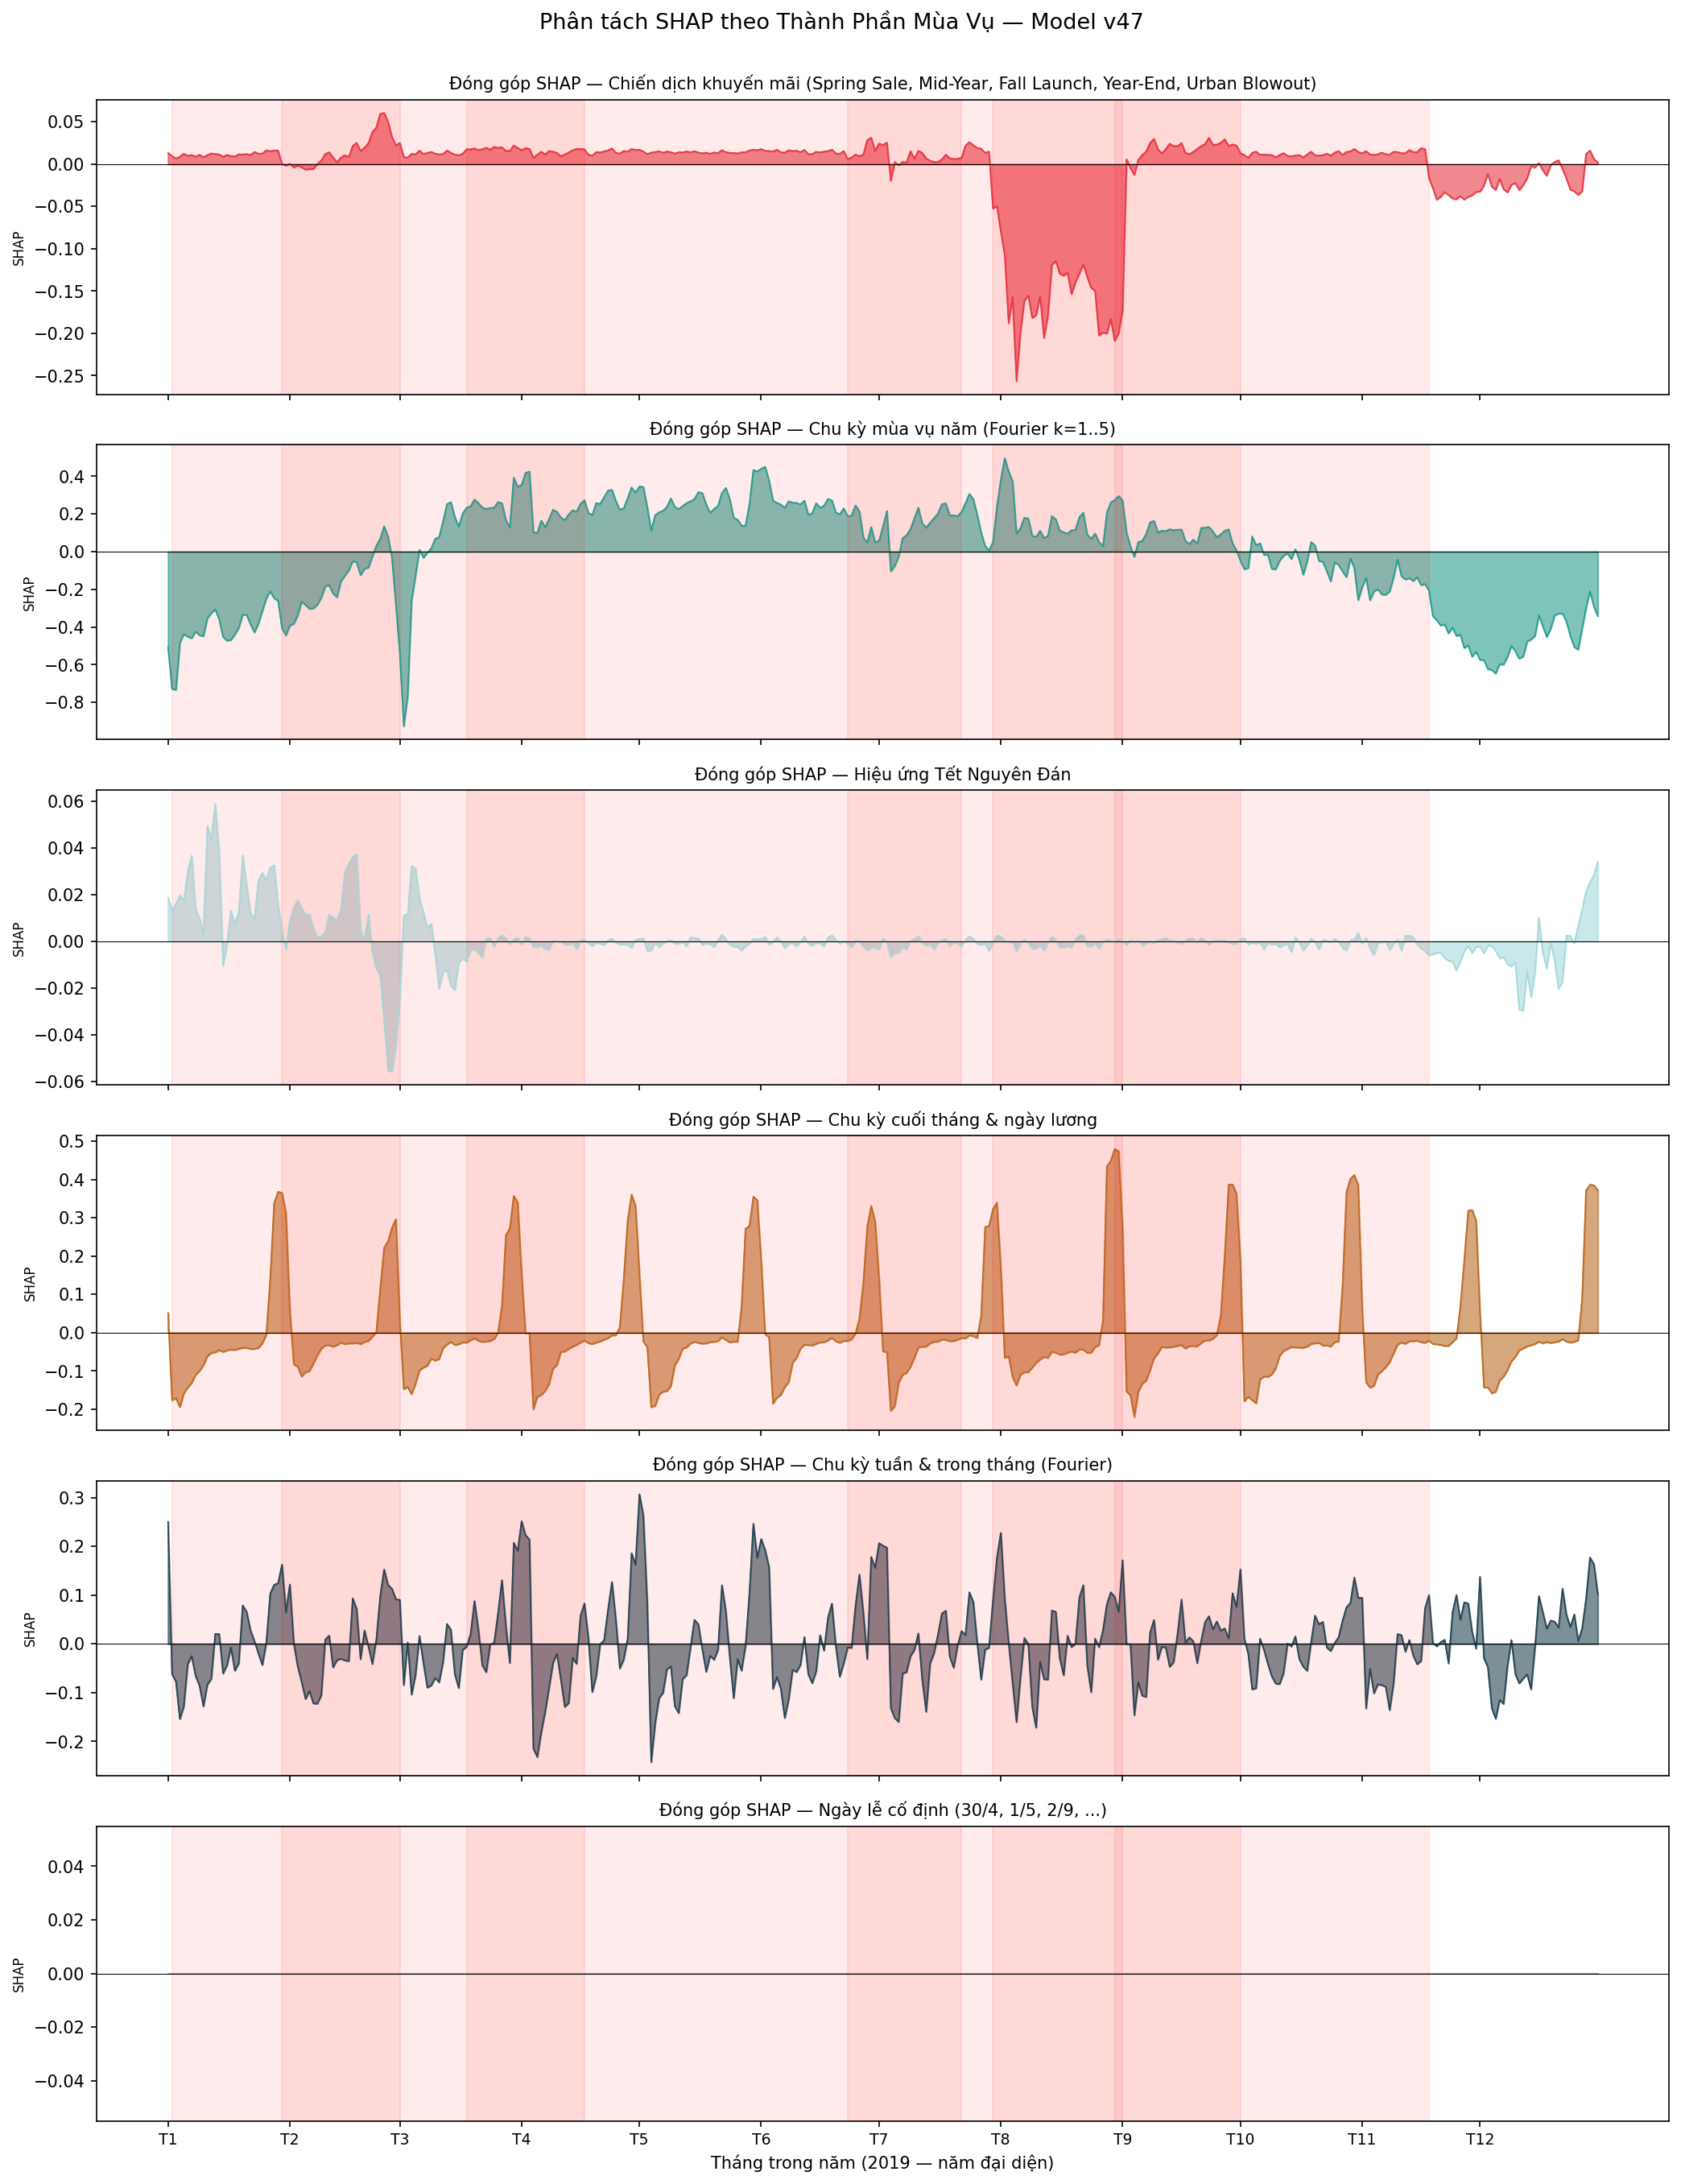
\includegraphics[width=\linewidth]{figures/shap/shap_seasonal_decomp.png}
\caption{\textbf{Phân tách SHAP thành phần mùa vụ (2019).} Fourier năm biên độ lớn nhất (±0,4–0,8). EOM/Lương spike ±0,3–0,5 mỗi cuối tháng. Urban Blowout (T8): SHAP âm ($-0,15$ đến $-0,25$) — nhận diện đúng event margin-negative.}
\label{fig:shap_seasonal}
\end{figure}

\begin{figure}[htbp]
\centering
\begin{subfigure}[b]{0.49\linewidth}
  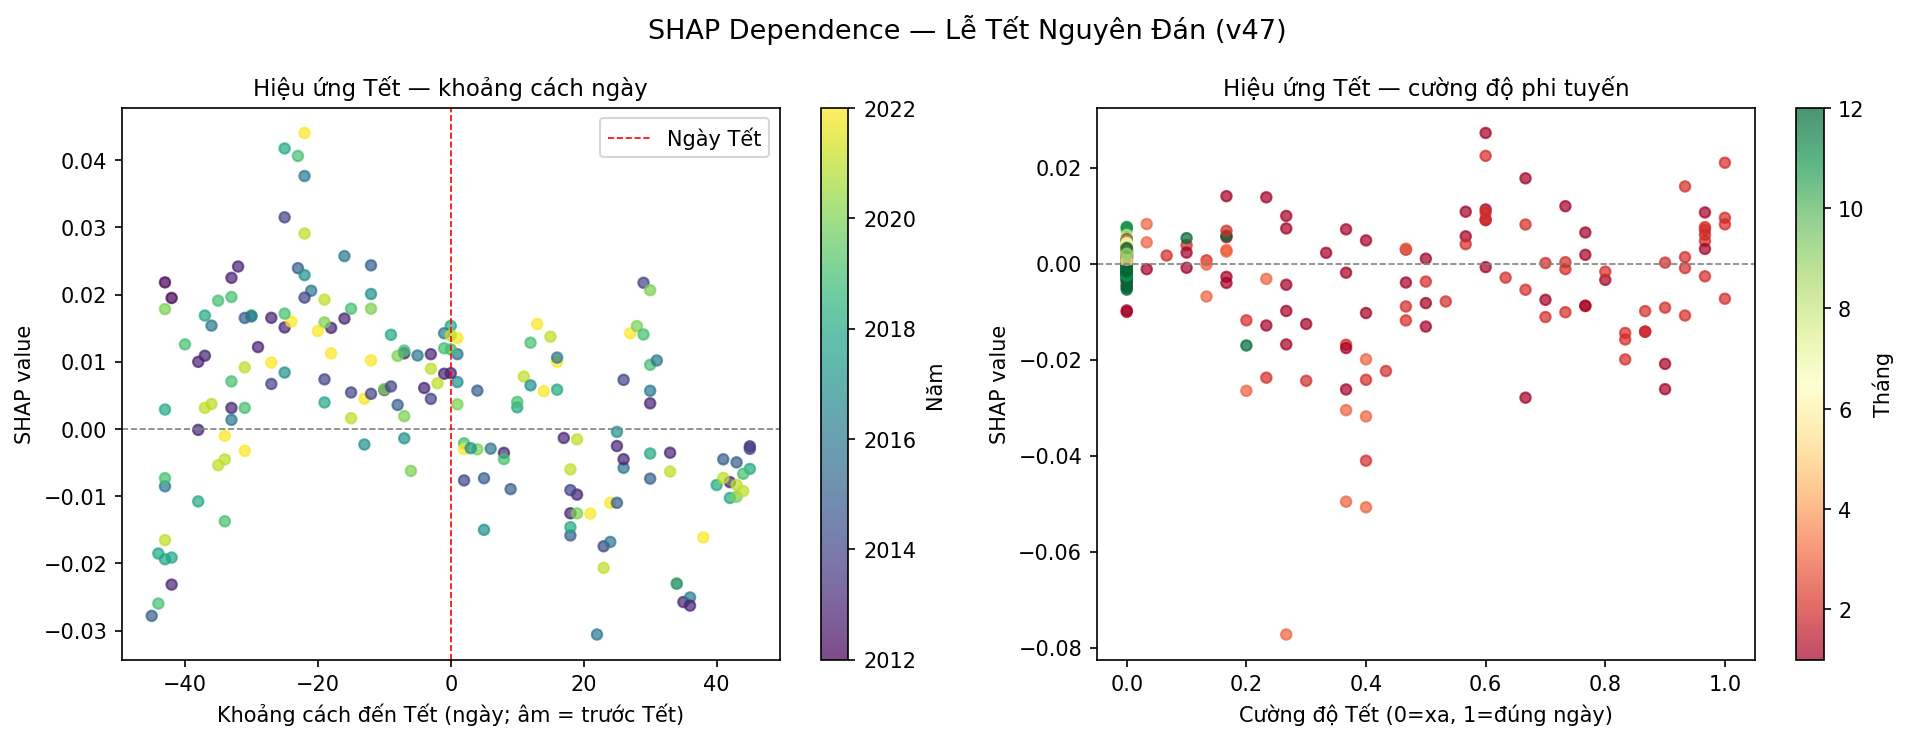
\includegraphics[width=\linewidth]{figures/shap/shap_dependence_tet.png}
  \caption{Tết phi tuyến: dương $-$30 đến $-$3 ngày, âm ngay sau Tết}
  \label{fig:shap_tet}
\end{subfigure}
\hfill
\begin{subfigure}[b]{0.49\linewidth}
  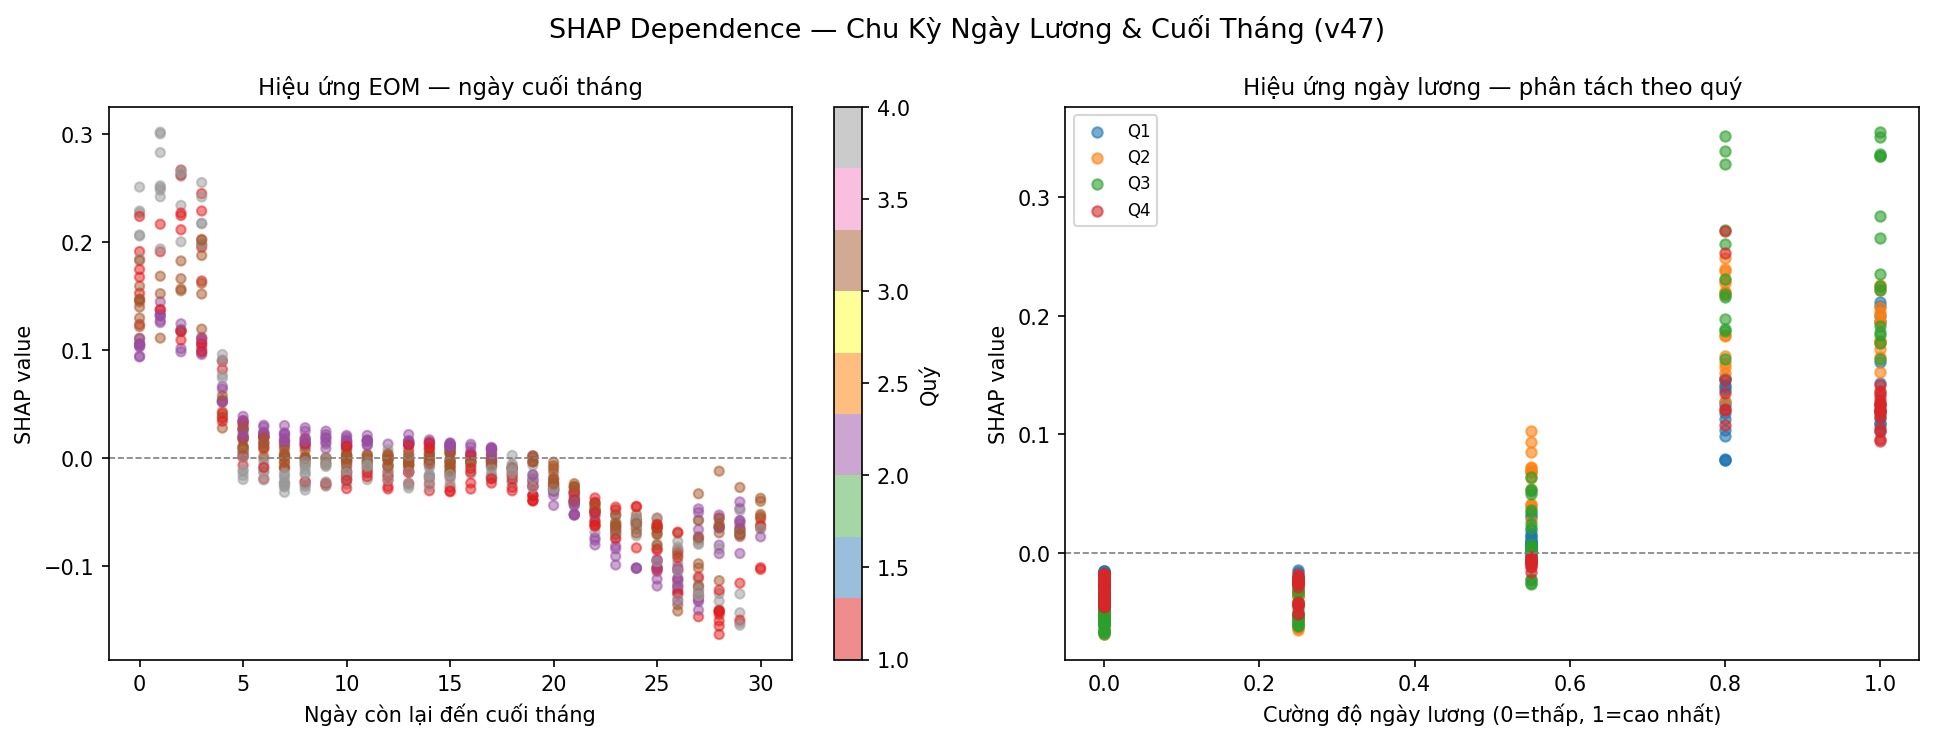
\includegraphics[width=\linewidth]{figures/shap/shap_dependence_eom_payday.png}
  \caption{EOM: SHAP giảm đơn điệu $+0,25$ (ngày 31) $\to$ $-0,10$ (đầu tháng)}
  \label{fig:shap_eom}
\end{subfigure}
\caption{SHAP Dependence: Tết và chu kỳ ngày lương.}
\end{figure}

\begin{figure}[htbp]
\centering
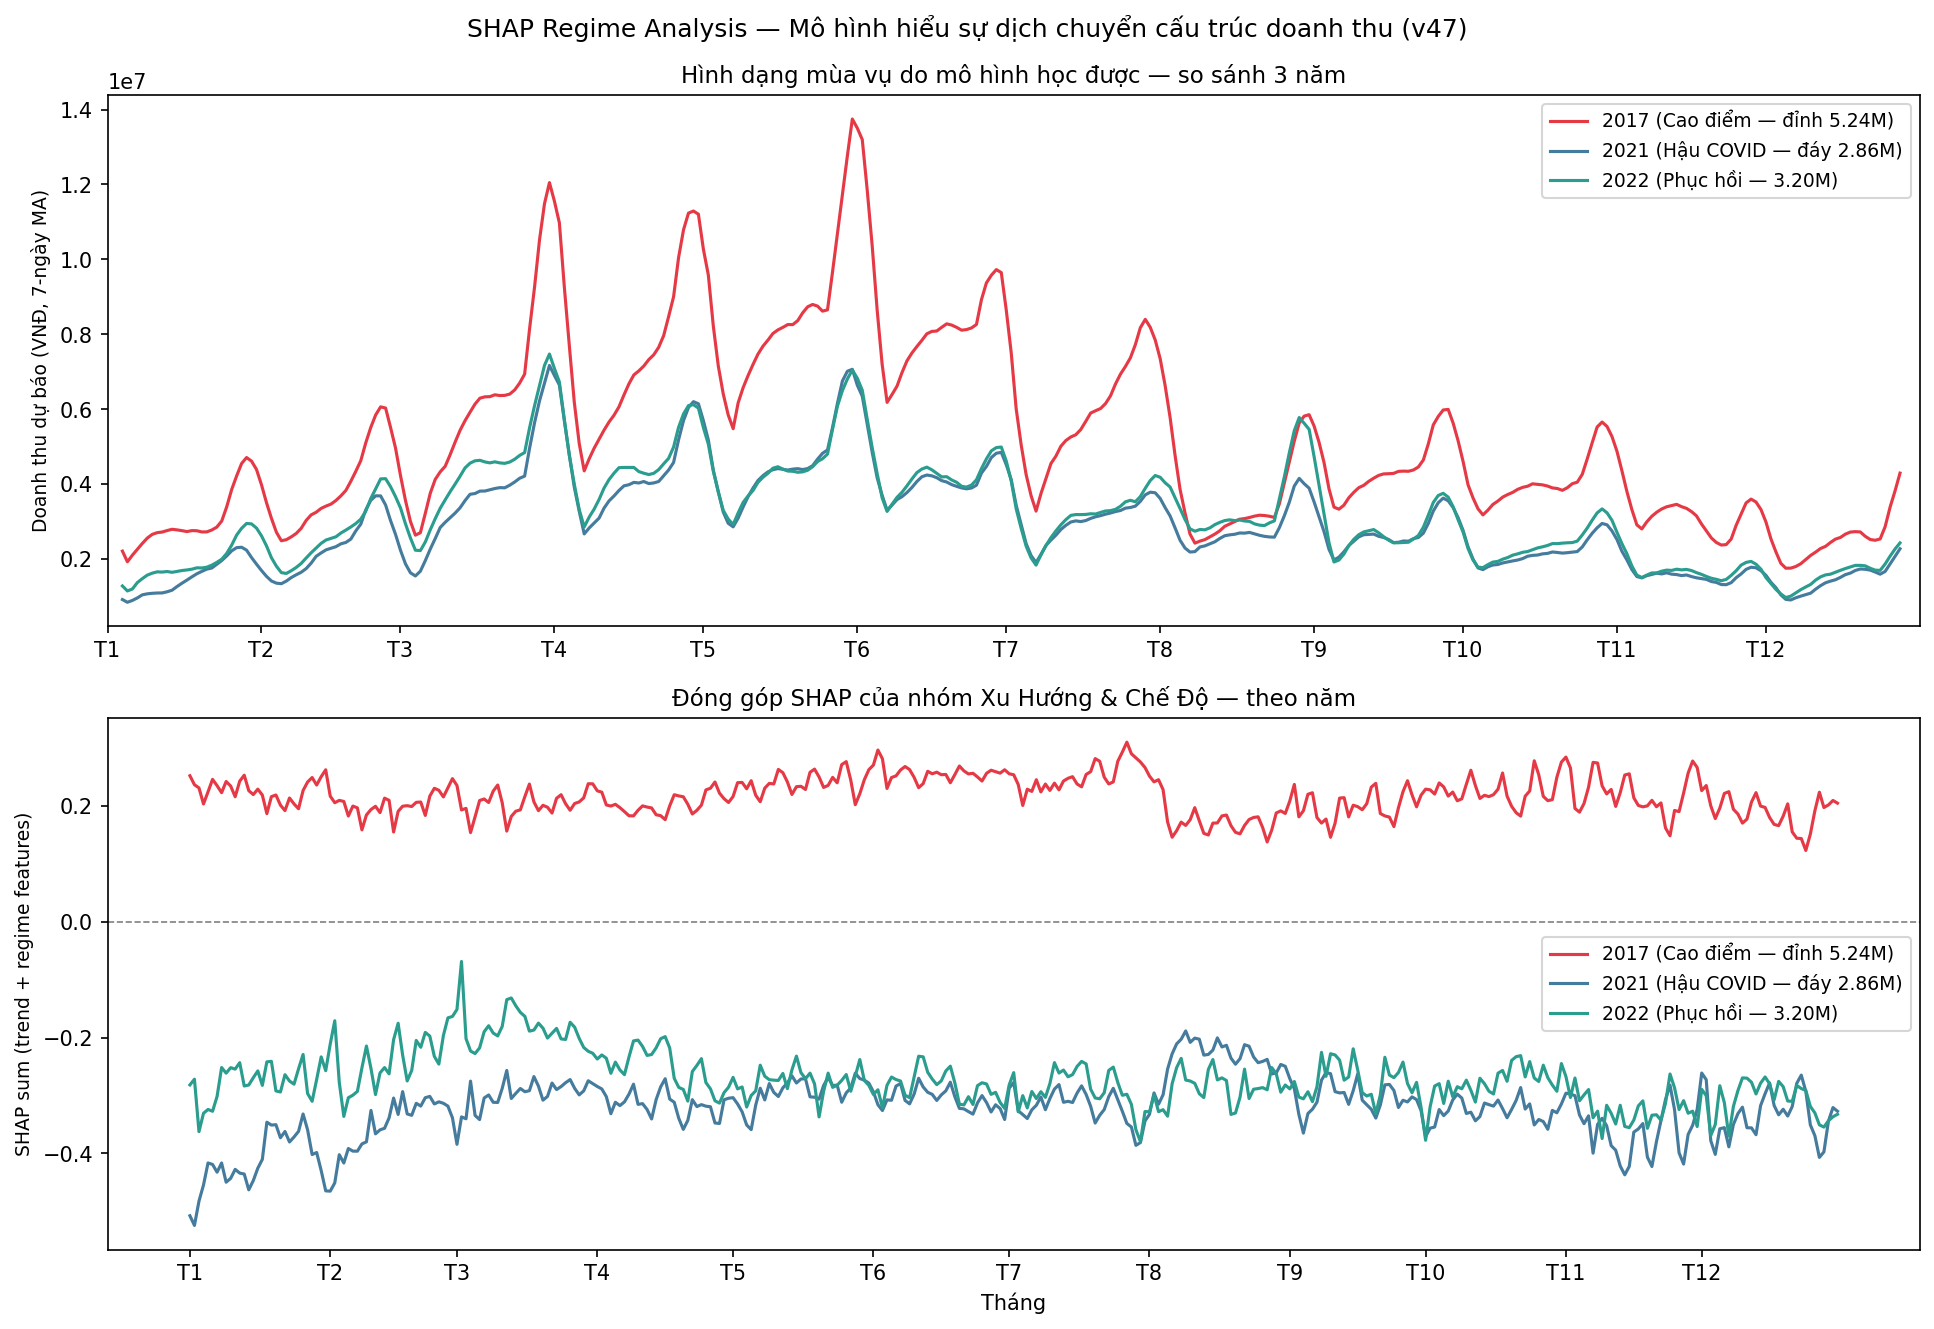
\includegraphics[width=0.9\linewidth]{figures/shap/shap_regime_comparison.png}
\caption{\textbf{SHAP regime analysis.} Shape mùa vụ giống nhau 2017/2021/2022, level khác nhau. SHAP trend delta $\approx$0,5 log-space $\equiv$ 1,65× revenue scale — cơ sở cho CR=1,2649.}
\label{fig:shap_regime}
\end{figure}

\begin{figure}[htbp]
\centering
\begin{subfigure}[b]{0.49\linewidth}
  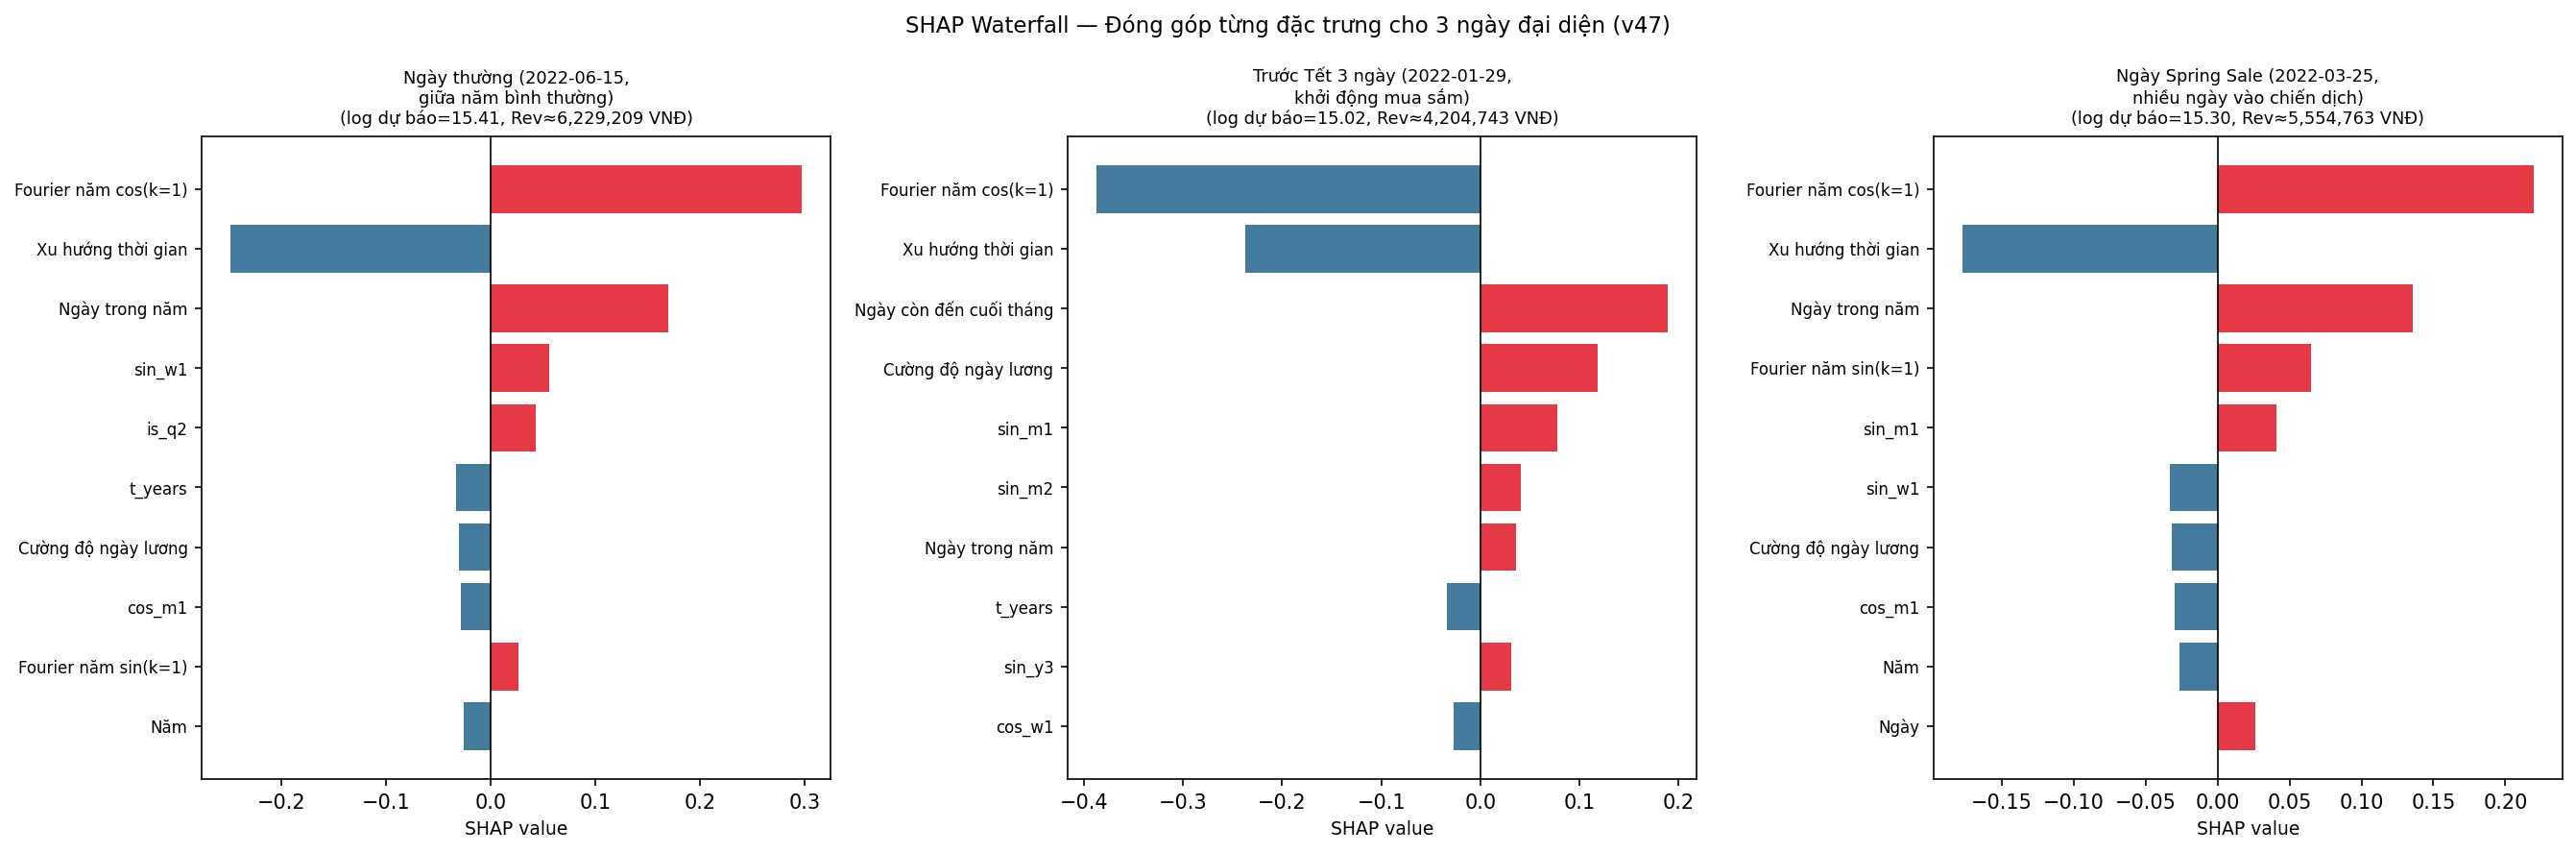
\includegraphics[width=\linewidth]{figures/shap/shap_waterfall_3days.png}
  \caption{Waterfall 3 ngày: thường (T6-15), trước Tết 3 ngày, ngày Spring Sale}
  \label{fig:shap_waterfall}
\end{subfigure}
\hfill
\begin{subfigure}[b]{0.49\linewidth}
  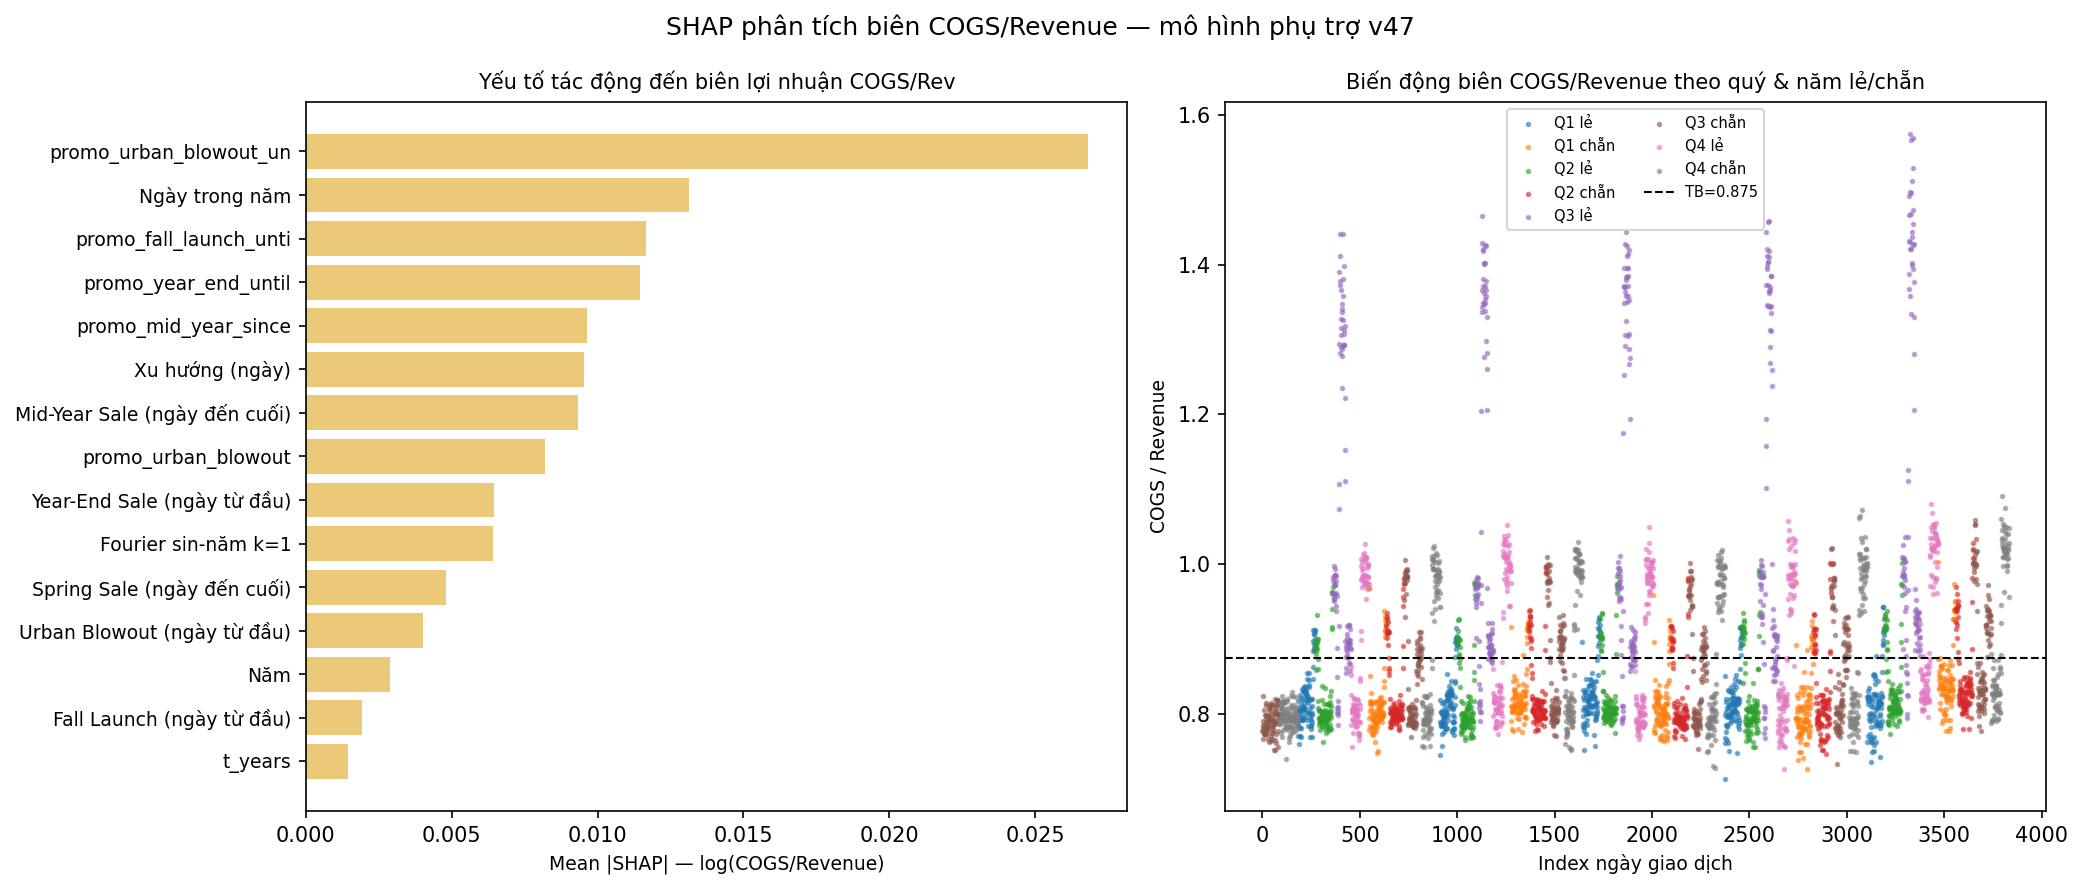
\includegraphics[width=\linewidth]{figures/shap/shap_margin_analysis.png}
  \caption{Margin SHAP: urban\_blowout\_until là driver chính của COGS/Rev}
  \label{fig:margin_shap}
\end{subfigure}
\caption{Waterfall đơn ngày và SHAP margin model.}
\end{figure}

\begin{figure}[htbp]
\centering
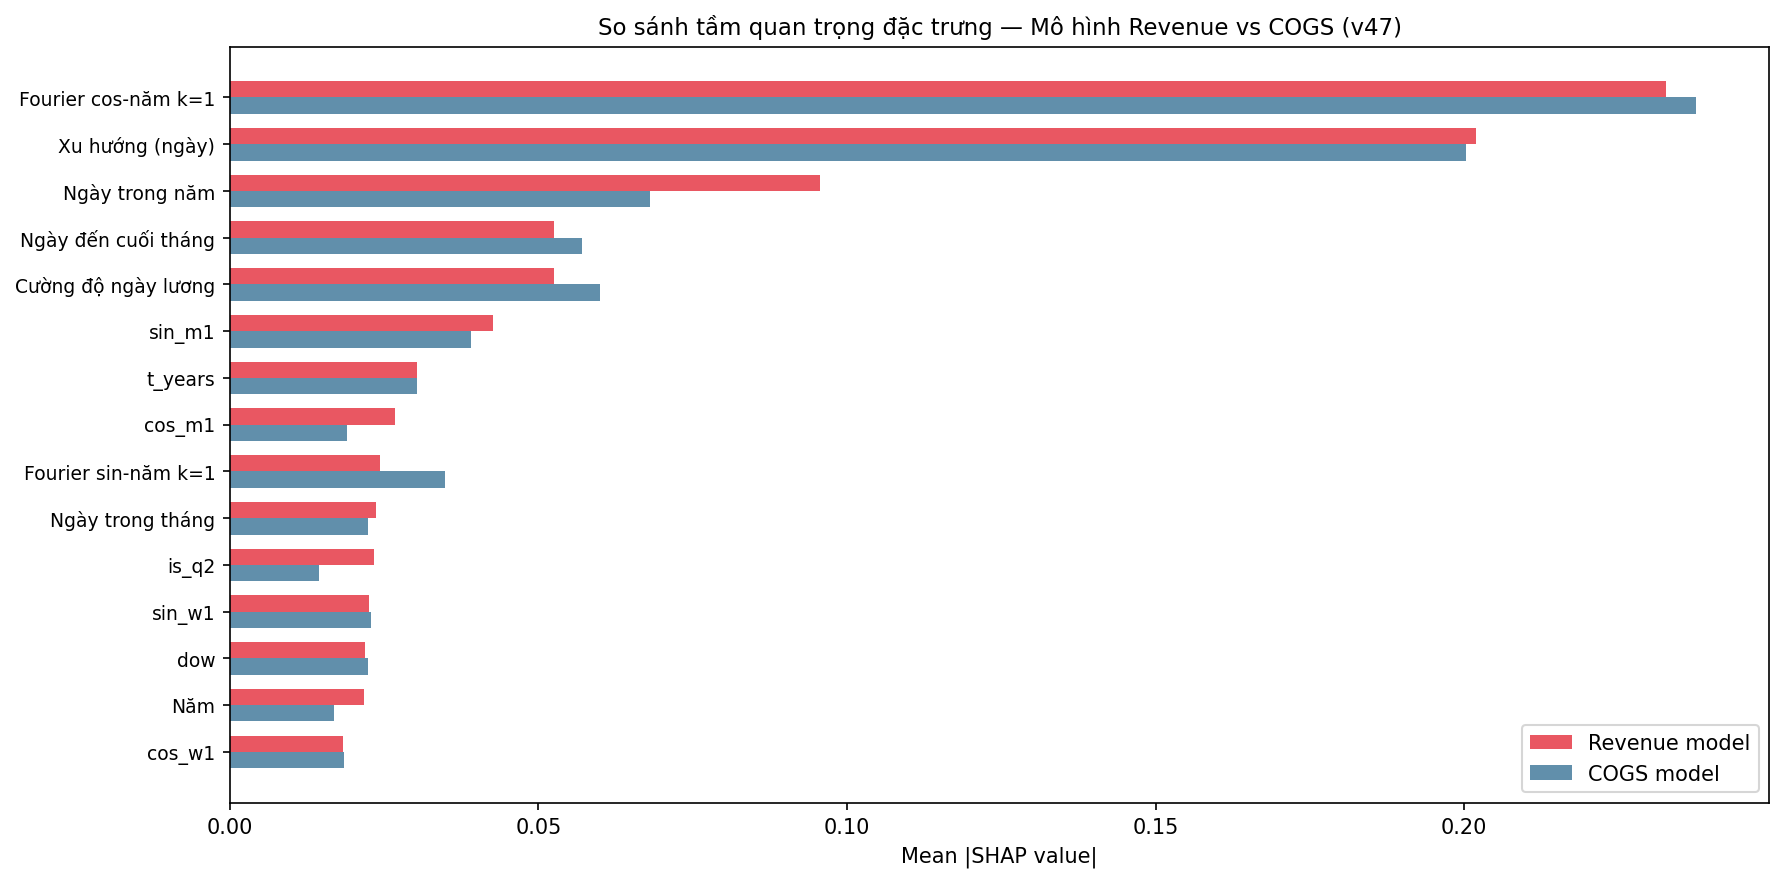
\includegraphics[width=\linewidth]{figures/shap/shap_cogs_vs_rev_comparison.png}
\caption{\textbf{Revenue vs COGS SHAP.} Top-2 giống nhau (cos\_y1, t\_days). COGS nhạy hơn với sin\_y1 (pha 90°) — biện hộ cho 2 model riêng biệt.}
\label{fig:cogs_rev_shap}
\end{figure}

\begin{figure}[htbp]
\centering
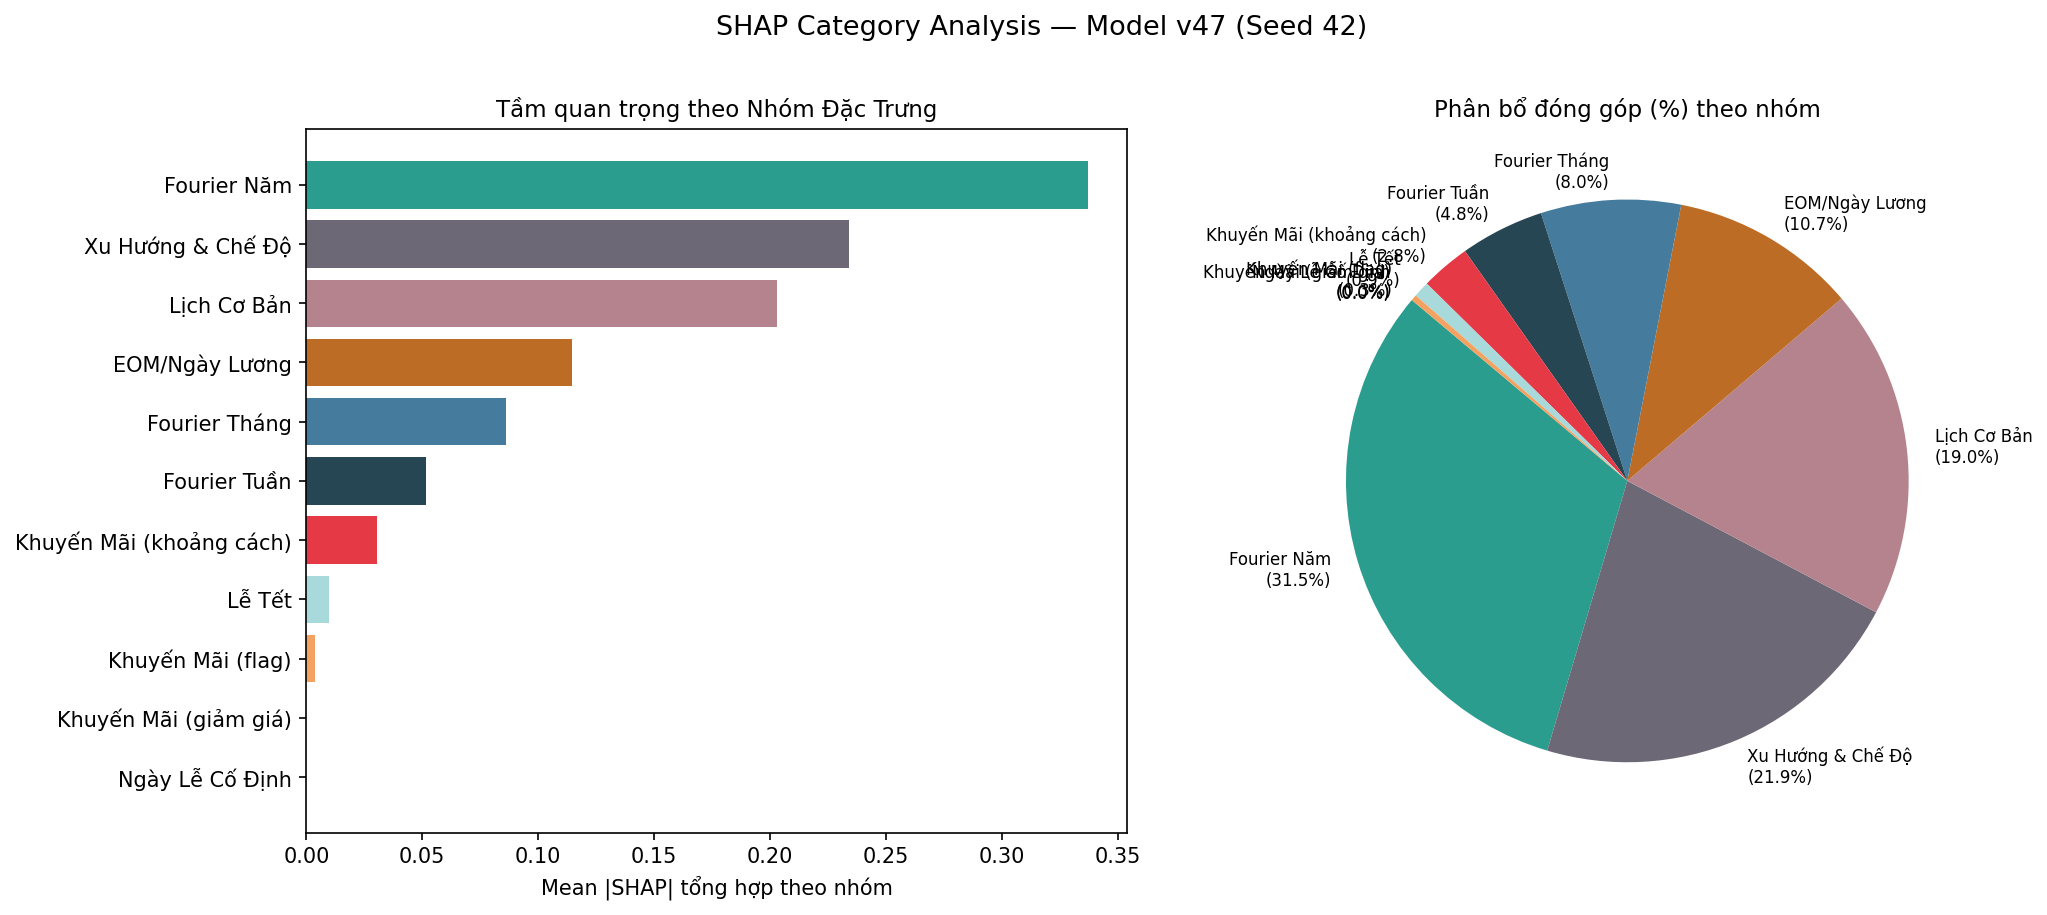
\includegraphics[width=0.85\linewidth]{figures/shap/shap_category_bar.png}
\caption{\textbf{SHAP theo nhóm.} Fourier Năm 31,5\% + Xu Hướng \& Chế Độ 21,9\% = 53,4\% — xác nhận mô hình học đúng cả shape lẫn level.}
\label{fig:shap_cat}
\end{figure}

\end{document}